\documentclass[12pt]{amsart}

\usepackage[utf8]{inputenc}
\usepackage{amsfonts}
\usepackage{amsthm}
\usepackage{amsmath}
\usepackage{amscd}
\usepackage{epstopdf}
\usepackage{csquotes}
\usepackage{enumitem}
\usepackage{mathrsfs}
\usepackage{pgfplots}
\usepackage{hyperref}

\pgfplotsset{compat=1.14}

\usepackage[draft]{todonotes}

\newcommand{\R}{\mathbb{R}}
\newcommand{\Z}{\mathbb{Z}}
\newcommand{\LP}{L^2(\mathbb{R})}
\newcommand{\norm}[1]{\left\lVert#1\right\rVert}
\newcommand{\abs}[1]{\left\lvert#1\right\rvert}

\newtheorem{thm}{Theorem}[section]
\newtheorem{corollary}{Corollary}[thm]
\newtheorem{lemma}[thm]{Lemma}
\newtheorem{case}{Case}
\usepackage{etoolbox}
\AtEndEnvironment{proof}{\setcounter{case}{0}}

\title{Wavelets}
\author{Grant Mohn \and Arden Rasmussen}
\date{\today}

\begin{document}
\pagenumbering{gobble}
\maketitle
\pagenumbering{arabic}

\section{Introduction}%
\label{sec:introduction}

Wavelets are a method for the representation of any function in
$\LP$. Similarly to how the Fourier series is used to represent
the same functions utilizing trigonometric functions, Wavelets are the same,
except instead of utilizing trigonometric functions, it is possible to use any
number of wavelets.

\section{Haar Wavelets}%
\label{sec:haar_wavelets}

It is possible to create a basis for $\LP$ using many different
wavelets.  However, for the scope of this paper, we will only focus on the
wavelet basis formed by the wavelets of the Haar function. The Haar function is
defined by

\begin{align}
  \Psi &= \begin{cases} 
    1  & 0\leq x < \frac{1}{2} \\
    -1 & \frac{1}{2} \leq x < 1 \\
    0  & \text{otherwise}
  \end{cases}\label{eq:haar}
\end{align}

\begin{figure}[htpb]
\begin{center}
\begin{tikzpicture}[scale=1, transform shape]
  \begin{axis}[
    axis lines = middle,
    xlabel = $x$,
    ylabel = {$f(x)$}]
  \addplot[domain=-.5:0, samples=100, line width=2pt]{0};
  \addplot[domain=0:.5, samples=100, line width=4pt]{1};
  \addplot[domain=.5:1, samples=100, line width=4pt]{-1};
  \addplot[domain=1:1.5, samples=100, line width=2pt]{0};
  \end{axis}
\end{tikzpicture}
\end{center}
\caption{Haar Function}
\label{fig:haar_function}
\end{figure}

A graph of the Haar function is shown in Figure~\ref{fig:haar_function}. A proposed basis for $\LP$ is

\begin{align}
  \Psi_{j,k} = \left\{2^{\frac{j}{2}}\Psi\left(2^jx-k\right)\right\}_{j\in\Z,\ k\in\Z}
\end{align}

This basis is the collection of Haar functions that are shifted by the $k$'s and stretched/compressed by the $j$'s. These two properties are demonstrated in Figure~\ref{fig:jk_diff}. Values of $k$ shift the graph of the function (left for negative values, and right for positive ones). Values of $j$ scale the function, positive values cause the function to be compressed along the $x$ axis, and stretched along the $y$ axis, and negative values cause the function to be stretched along the $x$ axis and compressed along the $y$ axis. This trade off between the stretching and compression of the axis, is to make the basis normal, and thus having unit ``length''.

\begin{figure}
% This file was created by matplotlib2tikz v0.6.16.
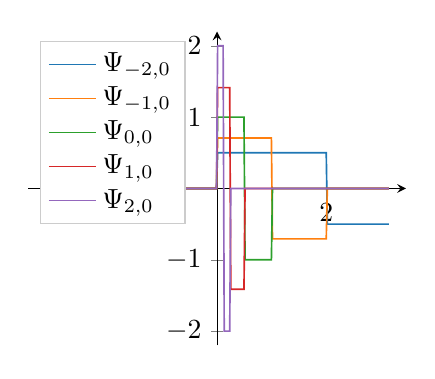
\begin{tikzpicture}

\definecolor{color0}{rgb}{0.12156862745098,0.466666666666667,0.705882352941177}
\definecolor{color1}{rgb}{1,0.498039215686275,0.0549019607843137}
\definecolor{color2}{rgb}{0.172549019607843,0.627450980392157,0.172549019607843}
\definecolor{color3}{rgb}{0.83921568627451,0.152941176470588,0.156862745098039}
\definecolor{color4}{rgb}{0.580392156862745,0.403921568627451,0.741176470588235}

\begin{axis}[
axis x line=center,
axis y line=center,
xmin=-3.45575191894877, xmax=3.45575191894877,
ymin=-2.2, ymax=2.2,
x grid style={white!69.01960784313725!black},
y grid style={white!69.01960784313725!black},
legend entries={{$\Psi_{-2,0}$},{$\Psi_{-1,0}$},{$\Psi_{0,0}$},{$\Psi_{1,0}$},{$\Psi_{2,0}$}},
legend cell align={left},
legend style={at={(0.03,0.97)}, anchor=north west, draw=white!80.0!black},
scale=.7
]
\addlegendimage{no markers, color0}
\addlegendimage{no markers, color1}
\addlegendimage{no markers, color2}
\addlegendimage{no markers, color3}
\addlegendimage{no markers, color4}
\addplot [semithick, color0]
table {%
-3.14159265358979 0
-3.12151857912596 0
-3.10144450466213 0
-3.0813704301983 0
-3.06129635573446 0
-3.04122228127063 0
-3.0211482068068 0
-3.00107413234297 0
-2.98100005787913 0
-2.9609259834153 0
-2.94085190895147 0
-2.92077783448764 0
-2.9007037600238 0
-2.88062968555997 0
-2.86055561109614 0
-2.8404815366323 0
-2.82040746216847 0
-2.80033338770464 0
-2.78025931324081 0
-2.76018523877697 0
-2.74011116431314 0
-2.72003708984931 0
-2.69996301538548 0
-2.67988894092164 0
-2.65981486645781 0
-2.63974079199398 0
-2.61966671753015 0
-2.59959264306631 0
-2.57951856860248 0
-2.55944449413865 0
-2.53937041967482 0
-2.51929634521098 0
-2.49922227074715 0
-2.47914819628332 0
-2.45907412181949 0
-2.43900004735565 0
-2.41892597289182 0
-2.39885189842799 0
-2.37877782396416 0
-2.35870374950032 0
-2.33862967503649 0
-2.31855560057266 0
-2.29848152610883 0
-2.27840745164499 0
-2.25833337718116 0
-2.23825930271733 0
-2.2181852282535 0
-2.19811115378966 0
-2.17803707932583 0
-2.157963004862 0
-2.13788893039817 0
-2.11781485593433 0
-2.0977407814705 0
-2.07766670700667 0
-2.05759263254284 0
-2.037518558079 0
-2.01744448361517 0
-1.99737040915134 0
-1.97729633468751 0
-1.95722226022367 0
-1.93714818575984 0
-1.91707411129601 0
-1.89700003683218 0
-1.87692596236834 0
-1.85685188790451 0
-1.83677781344068 0
-1.81670373897685 0
-1.79662966451301 0
-1.77655559004918 0
-1.75648151558535 0
-1.73640744112152 0
-1.71633336665768 0
-1.69625929219385 0
-1.67618521773002 0
-1.65611114326619 0
-1.63603706880235 0
-1.61596299433852 0
-1.59588891987469 0
-1.57581484541085 0
-1.55574077094702 0
-1.53566669648319 0
-1.51559262201936 0
-1.49551854755552 0
-1.47544447309169 0
-1.45537039862786 0
-1.43529632416403 0
-1.41522224970019 0
-1.39514817523636 0
-1.37507410077253 0
-1.3550000263087 0
-1.33492595184486 0
-1.31485187738103 0
-1.2947778029172 0
-1.27470372845337 0
-1.25462965398953 0
-1.2345555795257 0
-1.21448150506187 0
-1.19440743059804 0
-1.1743333561342 0
-1.15425928167037 0
-1.13418520720654 0
-1.11411113274271 0
-1.09403705827887 0
-1.07396298381504 0
-1.05388890935121 0
-1.03381483488738 0
-1.01374076042354 0
-0.993666685959711 0
-0.973592611495878 0
-0.953518537032046 0
-0.933444462568213 0
-0.913370388104381 0
-0.893296313640549 0
-0.873222239176716 0
-0.853148164712883 0
-0.833074090249051 0
-0.813000015785218 0
-0.792925941321386 0
-0.772851866857553 0
-0.75277779239372 0
-0.732703717929888 0
-0.712629643466055 0
-0.692555569002223 0
-0.672481494538391 0
-0.652407420074558 0
-0.632333345610725 0
-0.612259271146893 0
-0.59218519668306 0
-0.572111122219228 0
-0.552037047755395 0
-0.531962973291563 0
-0.51188889882773 0
-0.491814824363897 0
-0.471740749900065 0
-0.451666675436233 0
-0.4315926009724 0
-0.411518526508567 0
-0.391444452044735 0
-0.371370377580902 0
-0.35129630311707 0
-0.331222228653237 0
-0.311148154189405 0
-0.291074079725572 0
-0.271000005261739 0
-0.250925930797907 0
-0.230851856334074 0
-0.210777781870242 0
-0.19070370740641 0
-0.170629632942577 0
-0.150555558478744 0
-0.130481484014912 0
-0.110407409551079 0
-0.0903333350872466 0
-0.070259260623414 0
-0.0501851861595815 0
-0.0301111116957489 0
-0.0100370372319163 0
0.0100370372319163 0.5
0.0301111116957484 0.5
0.050185186159581 0.5
0.0702592606234136 0.5
0.0903333350872462 0.5
0.110407409551079 0.5
0.130481484014911 0.5
0.150555558478744 0.5
0.170629632942576 0.5
0.190703707406409 0.5
0.210777781870242 0.5
0.230851856334074 0.5
0.250925930797906 0.5
0.271000005261739 0.5
0.291074079725572 0.5
0.311148154189404 0.5
0.331222228653237 0.5
0.351296303117069 0.5
0.371370377580902 0.5
0.391444452044734 0.5
0.411518526508567 0.5
0.4315926009724 0.5
0.451666675436232 0.5
0.471740749900065 0.5
0.491814824363897 0.5
0.511888898827729 0.5
0.531962973291562 0.5
0.552037047755395 0.5
0.572111122219227 0.5
0.59218519668306 0.5
0.612259271146892 0.5
0.632333345610725 0.5
0.652407420074558 0.5
0.67248149453839 0.5
0.692555569002223 0.5
0.712629643466055 0.5
0.732703717929887 0.5
0.75277779239372 0.5
0.772851866857553 0.5
0.792925941321385 0.5
0.813000015785218 0.5
0.83307409024905 0.5
0.853148164712883 0.5
0.873222239176715 0.5
0.893296313640548 0.5
0.91337038810438 0.5
0.933444462568213 0.5
0.953518537032045 0.5
0.973592611495878 0.5
0.993666685959711 0.5
1.01374076042354 0.5
1.03381483488738 0.5
1.05388890935121 0.5
1.07396298381504 0.5
1.09403705827887 0.5
1.11411113274271 0.5
1.13418520720654 0.5
1.15425928167037 0.5
1.1743333561342 0.5
1.19440743059804 0.5
1.21448150506187 0.5
1.2345555795257 0.5
1.25462965398953 0.5
1.27470372845337 0.5
1.2947778029172 0.5
1.31485187738103 0.5
1.33492595184486 0.5
1.3550000263087 0.5
1.37507410077253 0.5
1.39514817523636 0.5
1.41522224970019 0.5
1.43529632416403 0.5
1.45537039862786 0.5
1.47544447309169 0.5
1.49551854755552 0.5
1.51559262201936 0.5
1.53566669648319 0.5
1.55574077094702 0.5
1.57581484541085 0.5
1.59588891987469 0.5
1.61596299433852 0.5
1.63603706880235 0.5
1.65611114326618 0.5
1.67618521773002 0.5
1.69625929219385 0.5
1.71633336665768 0.5
1.73640744112152 0.5
1.75648151558535 0.5
1.77655559004918 0.5
1.79662966451301 0.5
1.81670373897684 0.5
1.83677781344068 0.5
1.85685188790451 0.5
1.87692596236834 0.5
1.89700003683217 0.5
1.91707411129601 0.5
1.93714818575984 0.5
1.95722226022367 0.5
1.97729633468751 0.5
1.99737040915134 0.5
2.01744448361517 -0.5
2.037518558079 -0.5
2.05759263254284 -0.5
2.07766670700667 -0.5
2.0977407814705 -0.5
2.11781485593433 -0.5
2.13788893039817 -0.5
2.157963004862 -0.5
2.17803707932583 -0.5
2.19811115378966 -0.5
2.2181852282535 -0.5
2.23825930271733 -0.5
2.25833337718116 -0.5
2.27840745164499 -0.5
2.29848152610883 -0.5
2.31855560057266 -0.5
2.33862967503649 -0.5
2.35870374950032 -0.5
2.37877782396416 -0.5
2.39885189842799 -0.5
2.41892597289182 -0.5
2.43900004735565 -0.5
2.45907412181949 -0.5
2.47914819628332 -0.5
2.49922227074715 -0.5
2.51929634521098 -0.5
2.53937041967482 -0.5
2.55944449413865 -0.5
2.57951856860248 -0.5
2.59959264306631 -0.5
2.61966671753015 -0.5
2.63974079199398 -0.5
2.65981486645781 -0.5
2.67988894092164 -0.5
2.69996301538548 -0.5
2.72003708984931 -0.5
2.74011116431314 -0.5
2.76018523877697 -0.5
2.78025931324081 -0.5
2.80033338770464 -0.5
2.82040746216847 -0.5
2.8404815366323 -0.5
2.86055561109614 -0.5
2.88062968555997 -0.5
2.9007037600238 -0.5
2.92077783448763 -0.5
2.94085190895147 -0.5
2.9609259834153 -0.5
2.98100005787913 -0.5
3.00107413234297 -0.5
3.0211482068068 -0.5
3.04122228127063 -0.5
3.06129635573446 -0.5
3.0813704301983 -0.5
3.10144450466213 -0.5
3.12151857912596 -0.5
3.14159265358979 -0.5
};
\addplot [semithick, color1]
table {%
-3.14159265358979 0
-3.12151857912596 0
-3.10144450466213 0
-3.0813704301983 0
-3.06129635573446 0
-3.04122228127063 0
-3.0211482068068 0
-3.00107413234297 0
-2.98100005787913 0
-2.9609259834153 0
-2.94085190895147 0
-2.92077783448764 0
-2.9007037600238 0
-2.88062968555997 0
-2.86055561109614 0
-2.8404815366323 0
-2.82040746216847 0
-2.80033338770464 0
-2.78025931324081 0
-2.76018523877697 0
-2.74011116431314 0
-2.72003708984931 0
-2.69996301538548 0
-2.67988894092164 0
-2.65981486645781 0
-2.63974079199398 0
-2.61966671753015 0
-2.59959264306631 0
-2.57951856860248 0
-2.55944449413865 0
-2.53937041967482 0
-2.51929634521098 0
-2.49922227074715 0
-2.47914819628332 0
-2.45907412181949 0
-2.43900004735565 0
-2.41892597289182 0
-2.39885189842799 0
-2.37877782396416 0
-2.35870374950032 0
-2.33862967503649 0
-2.31855560057266 0
-2.29848152610883 0
-2.27840745164499 0
-2.25833337718116 0
-2.23825930271733 0
-2.2181852282535 0
-2.19811115378966 0
-2.17803707932583 0
-2.157963004862 0
-2.13788893039817 0
-2.11781485593433 0
-2.0977407814705 0
-2.07766670700667 0
-2.05759263254284 0
-2.037518558079 0
-2.01744448361517 0
-1.99737040915134 0
-1.97729633468751 0
-1.95722226022367 0
-1.93714818575984 0
-1.91707411129601 0
-1.89700003683218 0
-1.87692596236834 0
-1.85685188790451 0
-1.83677781344068 0
-1.81670373897685 0
-1.79662966451301 0
-1.77655559004918 0
-1.75648151558535 0
-1.73640744112152 0
-1.71633336665768 0
-1.69625929219385 0
-1.67618521773002 0
-1.65611114326619 0
-1.63603706880235 0
-1.61596299433852 0
-1.59588891987469 0
-1.57581484541085 0
-1.55574077094702 0
-1.53566669648319 0
-1.51559262201936 0
-1.49551854755552 0
-1.47544447309169 0
-1.45537039862786 0
-1.43529632416403 0
-1.41522224970019 0
-1.39514817523636 0
-1.37507410077253 0
-1.3550000263087 0
-1.33492595184486 0
-1.31485187738103 0
-1.2947778029172 0
-1.27470372845337 0
-1.25462965398953 0
-1.2345555795257 0
-1.21448150506187 0
-1.19440743059804 0
-1.1743333561342 0
-1.15425928167037 0
-1.13418520720654 0
-1.11411113274271 0
-1.09403705827887 0
-1.07396298381504 0
-1.05388890935121 0
-1.03381483488738 0
-1.01374076042354 0
-0.993666685959711 0
-0.973592611495878 0
-0.953518537032046 0
-0.933444462568213 0
-0.913370388104381 0
-0.893296313640549 0
-0.873222239176716 0
-0.853148164712883 0
-0.833074090249051 0
-0.813000015785218 0
-0.792925941321386 0
-0.772851866857553 0
-0.75277779239372 0
-0.732703717929888 0
-0.712629643466055 0
-0.692555569002223 0
-0.672481494538391 0
-0.652407420074558 0
-0.632333345610725 0
-0.612259271146893 0
-0.59218519668306 0
-0.572111122219228 0
-0.552037047755395 0
-0.531962973291563 0
-0.51188889882773 0
-0.491814824363897 0
-0.471740749900065 0
-0.451666675436233 0
-0.4315926009724 0
-0.411518526508567 0
-0.391444452044735 0
-0.371370377580902 0
-0.35129630311707 0
-0.331222228653237 0
-0.311148154189405 0
-0.291074079725572 0
-0.271000005261739 0
-0.250925930797907 0
-0.230851856334074 0
-0.210777781870242 0
-0.19070370740641 0
-0.170629632942577 0
-0.150555558478744 0
-0.130481484014912 0
-0.110407409551079 0
-0.0903333350872466 0
-0.070259260623414 0
-0.0501851861595815 0
-0.0301111116957489 0
-0.0100370372319163 0
0.0100370372319163 0.707106781186548
0.0301111116957484 0.707106781186548
0.050185186159581 0.707106781186548
0.0702592606234136 0.707106781186548
0.0903333350872462 0.707106781186548
0.110407409551079 0.707106781186548
0.130481484014911 0.707106781186548
0.150555558478744 0.707106781186548
0.170629632942576 0.707106781186548
0.190703707406409 0.707106781186548
0.210777781870242 0.707106781186548
0.230851856334074 0.707106781186548
0.250925930797906 0.707106781186548
0.271000005261739 0.707106781186548
0.291074079725572 0.707106781186548
0.311148154189404 0.707106781186548
0.331222228653237 0.707106781186548
0.351296303117069 0.707106781186548
0.371370377580902 0.707106781186548
0.391444452044734 0.707106781186548
0.411518526508567 0.707106781186548
0.4315926009724 0.707106781186548
0.451666675436232 0.707106781186548
0.471740749900065 0.707106781186548
0.491814824363897 0.707106781186548
0.511888898827729 0.707106781186548
0.531962973291562 0.707106781186548
0.552037047755395 0.707106781186548
0.572111122219227 0.707106781186548
0.59218519668306 0.707106781186548
0.612259271146892 0.707106781186548
0.632333345610725 0.707106781186548
0.652407420074558 0.707106781186548
0.67248149453839 0.707106781186548
0.692555569002223 0.707106781186548
0.712629643466055 0.707106781186548
0.732703717929887 0.707106781186548
0.75277779239372 0.707106781186548
0.772851866857553 0.707106781186548
0.792925941321385 0.707106781186548
0.813000015785218 0.707106781186548
0.83307409024905 0.707106781186548
0.853148164712883 0.707106781186548
0.873222239176715 0.707106781186548
0.893296313640548 0.707106781186548
0.91337038810438 0.707106781186548
0.933444462568213 0.707106781186548
0.953518537032045 0.707106781186548
0.973592611495878 0.707106781186548
0.993666685959711 0.707106781186548
1.01374076042354 -0.707106781186548
1.03381483488738 -0.707106781186548
1.05388890935121 -0.707106781186548
1.07396298381504 -0.707106781186548
1.09403705827887 -0.707106781186548
1.11411113274271 -0.707106781186548
1.13418520720654 -0.707106781186548
1.15425928167037 -0.707106781186548
1.1743333561342 -0.707106781186548
1.19440743059804 -0.707106781186548
1.21448150506187 -0.707106781186548
1.2345555795257 -0.707106781186548
1.25462965398953 -0.707106781186548
1.27470372845337 -0.707106781186548
1.2947778029172 -0.707106781186548
1.31485187738103 -0.707106781186548
1.33492595184486 -0.707106781186548
1.3550000263087 -0.707106781186548
1.37507410077253 -0.707106781186548
1.39514817523636 -0.707106781186548
1.41522224970019 -0.707106781186548
1.43529632416403 -0.707106781186548
1.45537039862786 -0.707106781186548
1.47544447309169 -0.707106781186548
1.49551854755552 -0.707106781186548
1.51559262201936 -0.707106781186548
1.53566669648319 -0.707106781186548
1.55574077094702 -0.707106781186548
1.57581484541085 -0.707106781186548
1.59588891987469 -0.707106781186548
1.61596299433852 -0.707106781186548
1.63603706880235 -0.707106781186548
1.65611114326618 -0.707106781186548
1.67618521773002 -0.707106781186548
1.69625929219385 -0.707106781186548
1.71633336665768 -0.707106781186548
1.73640744112152 -0.707106781186548
1.75648151558535 -0.707106781186548
1.77655559004918 -0.707106781186548
1.79662966451301 -0.707106781186548
1.81670373897684 -0.707106781186548
1.83677781344068 -0.707106781186548
1.85685188790451 -0.707106781186548
1.87692596236834 -0.707106781186548
1.89700003683217 -0.707106781186548
1.91707411129601 -0.707106781186548
1.93714818575984 -0.707106781186548
1.95722226022367 -0.707106781186548
1.97729633468751 -0.707106781186548
1.99737040915134 -0.707106781186548
2.01744448361517 0
2.037518558079 0
2.05759263254284 0
2.07766670700667 0
2.0977407814705 0
2.11781485593433 0
2.13788893039817 0
2.157963004862 0
2.17803707932583 0
2.19811115378966 0
2.2181852282535 0
2.23825930271733 0
2.25833337718116 0
2.27840745164499 0
2.29848152610883 0
2.31855560057266 0
2.33862967503649 0
2.35870374950032 0
2.37877782396416 0
2.39885189842799 0
2.41892597289182 0
2.43900004735565 0
2.45907412181949 0
2.47914819628332 0
2.49922227074715 0
2.51929634521098 0
2.53937041967482 0
2.55944449413865 0
2.57951856860248 0
2.59959264306631 0
2.61966671753015 0
2.63974079199398 0
2.65981486645781 0
2.67988894092164 0
2.69996301538548 0
2.72003708984931 0
2.74011116431314 0
2.76018523877697 0
2.78025931324081 0
2.80033338770464 0
2.82040746216847 0
2.8404815366323 0
2.86055561109614 0
2.88062968555997 0
2.9007037600238 0
2.92077783448763 0
2.94085190895147 0
2.9609259834153 0
2.98100005787913 0
3.00107413234297 0
3.0211482068068 0
3.04122228127063 0
3.06129635573446 0
3.0813704301983 0
3.10144450466213 0
3.12151857912596 0
3.14159265358979 0
};
\addplot [semithick, color2]
table {%
-3.14159265358979 0
-3.12151857912596 0
-3.10144450466213 0
-3.0813704301983 0
-3.06129635573446 0
-3.04122228127063 0
-3.0211482068068 0
-3.00107413234297 0
-2.98100005787913 0
-2.9609259834153 0
-2.94085190895147 0
-2.92077783448764 0
-2.9007037600238 0
-2.88062968555997 0
-2.86055561109614 0
-2.8404815366323 0
-2.82040746216847 0
-2.80033338770464 0
-2.78025931324081 0
-2.76018523877697 0
-2.74011116431314 0
-2.72003708984931 0
-2.69996301538548 0
-2.67988894092164 0
-2.65981486645781 0
-2.63974079199398 0
-2.61966671753015 0
-2.59959264306631 0
-2.57951856860248 0
-2.55944449413865 0
-2.53937041967482 0
-2.51929634521098 0
-2.49922227074715 0
-2.47914819628332 0
-2.45907412181949 0
-2.43900004735565 0
-2.41892597289182 0
-2.39885189842799 0
-2.37877782396416 0
-2.35870374950032 0
-2.33862967503649 0
-2.31855560057266 0
-2.29848152610883 0
-2.27840745164499 0
-2.25833337718116 0
-2.23825930271733 0
-2.2181852282535 0
-2.19811115378966 0
-2.17803707932583 0
-2.157963004862 0
-2.13788893039817 0
-2.11781485593433 0
-2.0977407814705 0
-2.07766670700667 0
-2.05759263254284 0
-2.037518558079 0
-2.01744448361517 0
-1.99737040915134 0
-1.97729633468751 0
-1.95722226022367 0
-1.93714818575984 0
-1.91707411129601 0
-1.89700003683218 0
-1.87692596236834 0
-1.85685188790451 0
-1.83677781344068 0
-1.81670373897685 0
-1.79662966451301 0
-1.77655559004918 0
-1.75648151558535 0
-1.73640744112152 0
-1.71633336665768 0
-1.69625929219385 0
-1.67618521773002 0
-1.65611114326619 0
-1.63603706880235 0
-1.61596299433852 0
-1.59588891987469 0
-1.57581484541085 0
-1.55574077094702 0
-1.53566669648319 0
-1.51559262201936 0
-1.49551854755552 0
-1.47544447309169 0
-1.45537039862786 0
-1.43529632416403 0
-1.41522224970019 0
-1.39514817523636 0
-1.37507410077253 0
-1.3550000263087 0
-1.33492595184486 0
-1.31485187738103 0
-1.2947778029172 0
-1.27470372845337 0
-1.25462965398953 0
-1.2345555795257 0
-1.21448150506187 0
-1.19440743059804 0
-1.1743333561342 0
-1.15425928167037 0
-1.13418520720654 0
-1.11411113274271 0
-1.09403705827887 0
-1.07396298381504 0
-1.05388890935121 0
-1.03381483488738 0
-1.01374076042354 0
-0.993666685959711 0
-0.973592611495878 0
-0.953518537032046 0
-0.933444462568213 0
-0.913370388104381 0
-0.893296313640549 0
-0.873222239176716 0
-0.853148164712883 0
-0.833074090249051 0
-0.813000015785218 0
-0.792925941321386 0
-0.772851866857553 0
-0.75277779239372 0
-0.732703717929888 0
-0.712629643466055 0
-0.692555569002223 0
-0.672481494538391 0
-0.652407420074558 0
-0.632333345610725 0
-0.612259271146893 0
-0.59218519668306 0
-0.572111122219228 0
-0.552037047755395 0
-0.531962973291563 0
-0.51188889882773 0
-0.491814824363897 0
-0.471740749900065 0
-0.451666675436233 0
-0.4315926009724 0
-0.411518526508567 0
-0.391444452044735 0
-0.371370377580902 0
-0.35129630311707 0
-0.331222228653237 0
-0.311148154189405 0
-0.291074079725572 0
-0.271000005261739 0
-0.250925930797907 0
-0.230851856334074 0
-0.210777781870242 0
-0.19070370740641 0
-0.170629632942577 0
-0.150555558478744 0
-0.130481484014912 0
-0.110407409551079 0
-0.0903333350872466 0
-0.070259260623414 0
-0.0501851861595815 0
-0.0301111116957489 0
-0.0100370372319163 0
0.0100370372319163 1
0.0301111116957484 1
0.050185186159581 1
0.0702592606234136 1
0.0903333350872462 1
0.110407409551079 1
0.130481484014911 1
0.150555558478744 1
0.170629632942576 1
0.190703707406409 1
0.210777781870242 1
0.230851856334074 1
0.250925930797906 1
0.271000005261739 1
0.291074079725572 1
0.311148154189404 1
0.331222228653237 1
0.351296303117069 1
0.371370377580902 1
0.391444452044734 1
0.411518526508567 1
0.4315926009724 1
0.451666675436232 1
0.471740749900065 1
0.491814824363897 1
0.511888898827729 -1
0.531962973291562 -1
0.552037047755395 -1
0.572111122219227 -1
0.59218519668306 -1
0.612259271146892 -1
0.632333345610725 -1
0.652407420074558 -1
0.67248149453839 -1
0.692555569002223 -1
0.712629643466055 -1
0.732703717929887 -1
0.75277779239372 -1
0.772851866857553 -1
0.792925941321385 -1
0.813000015785218 -1
0.83307409024905 -1
0.853148164712883 -1
0.873222239176715 -1
0.893296313640548 -1
0.91337038810438 -1
0.933444462568213 -1
0.953518537032045 -1
0.973592611495878 -1
0.993666685959711 -1
1.01374076042354 0
1.03381483488738 0
1.05388890935121 0
1.07396298381504 0
1.09403705827887 0
1.11411113274271 0
1.13418520720654 0
1.15425928167037 0
1.1743333561342 0
1.19440743059804 0
1.21448150506187 0
1.2345555795257 0
1.25462965398953 0
1.27470372845337 0
1.2947778029172 0
1.31485187738103 0
1.33492595184486 0
1.3550000263087 0
1.37507410077253 0
1.39514817523636 0
1.41522224970019 0
1.43529632416403 0
1.45537039862786 0
1.47544447309169 0
1.49551854755552 0
1.51559262201936 0
1.53566669648319 0
1.55574077094702 0
1.57581484541085 0
1.59588891987469 0
1.61596299433852 0
1.63603706880235 0
1.65611114326618 0
1.67618521773002 0
1.69625929219385 0
1.71633336665768 0
1.73640744112152 0
1.75648151558535 0
1.77655559004918 0
1.79662966451301 0
1.81670373897684 0
1.83677781344068 0
1.85685188790451 0
1.87692596236834 0
1.89700003683217 0
1.91707411129601 0
1.93714818575984 0
1.95722226022367 0
1.97729633468751 0
1.99737040915134 0
2.01744448361517 0
2.037518558079 0
2.05759263254284 0
2.07766670700667 0
2.0977407814705 0
2.11781485593433 0
2.13788893039817 0
2.157963004862 0
2.17803707932583 0
2.19811115378966 0
2.2181852282535 0
2.23825930271733 0
2.25833337718116 0
2.27840745164499 0
2.29848152610883 0
2.31855560057266 0
2.33862967503649 0
2.35870374950032 0
2.37877782396416 0
2.39885189842799 0
2.41892597289182 0
2.43900004735565 0
2.45907412181949 0
2.47914819628332 0
2.49922227074715 0
2.51929634521098 0
2.53937041967482 0
2.55944449413865 0
2.57951856860248 0
2.59959264306631 0
2.61966671753015 0
2.63974079199398 0
2.65981486645781 0
2.67988894092164 0
2.69996301538548 0
2.72003708984931 0
2.74011116431314 0
2.76018523877697 0
2.78025931324081 0
2.80033338770464 0
2.82040746216847 0
2.8404815366323 0
2.86055561109614 0
2.88062968555997 0
2.9007037600238 0
2.92077783448763 0
2.94085190895147 0
2.9609259834153 0
2.98100005787913 0
3.00107413234297 0
3.0211482068068 0
3.04122228127063 0
3.06129635573446 0
3.0813704301983 0
3.10144450466213 0
3.12151857912596 0
3.14159265358979 0
};
\addplot [semithick, color3]
table {%
-3.14159265358979 0
-3.12151857912596 0
-3.10144450466213 0
-3.0813704301983 0
-3.06129635573446 0
-3.04122228127063 0
-3.0211482068068 0
-3.00107413234297 0
-2.98100005787913 0
-2.9609259834153 0
-2.94085190895147 0
-2.92077783448764 0
-2.9007037600238 0
-2.88062968555997 0
-2.86055561109614 0
-2.8404815366323 0
-2.82040746216847 0
-2.80033338770464 0
-2.78025931324081 0
-2.76018523877697 0
-2.74011116431314 0
-2.72003708984931 0
-2.69996301538548 0
-2.67988894092164 0
-2.65981486645781 0
-2.63974079199398 0
-2.61966671753015 0
-2.59959264306631 0
-2.57951856860248 0
-2.55944449413865 0
-2.53937041967482 0
-2.51929634521098 0
-2.49922227074715 0
-2.47914819628332 0
-2.45907412181949 0
-2.43900004735565 0
-2.41892597289182 0
-2.39885189842799 0
-2.37877782396416 0
-2.35870374950032 0
-2.33862967503649 0
-2.31855560057266 0
-2.29848152610883 0
-2.27840745164499 0
-2.25833337718116 0
-2.23825930271733 0
-2.2181852282535 0
-2.19811115378966 0
-2.17803707932583 0
-2.157963004862 0
-2.13788893039817 0
-2.11781485593433 0
-2.0977407814705 0
-2.07766670700667 0
-2.05759263254284 0
-2.037518558079 0
-2.01744448361517 0
-1.99737040915134 0
-1.97729633468751 0
-1.95722226022367 0
-1.93714818575984 0
-1.91707411129601 0
-1.89700003683218 0
-1.87692596236834 0
-1.85685188790451 0
-1.83677781344068 0
-1.81670373897685 0
-1.79662966451301 0
-1.77655559004918 0
-1.75648151558535 0
-1.73640744112152 0
-1.71633336665768 0
-1.69625929219385 0
-1.67618521773002 0
-1.65611114326619 0
-1.63603706880235 0
-1.61596299433852 0
-1.59588891987469 0
-1.57581484541085 0
-1.55574077094702 0
-1.53566669648319 0
-1.51559262201936 0
-1.49551854755552 0
-1.47544447309169 0
-1.45537039862786 0
-1.43529632416403 0
-1.41522224970019 0
-1.39514817523636 0
-1.37507410077253 0
-1.3550000263087 0
-1.33492595184486 0
-1.31485187738103 0
-1.2947778029172 0
-1.27470372845337 0
-1.25462965398953 0
-1.2345555795257 0
-1.21448150506187 0
-1.19440743059804 0
-1.1743333561342 0
-1.15425928167037 0
-1.13418520720654 0
-1.11411113274271 0
-1.09403705827887 0
-1.07396298381504 0
-1.05388890935121 0
-1.03381483488738 0
-1.01374076042354 0
-0.993666685959711 0
-0.973592611495878 0
-0.953518537032046 0
-0.933444462568213 0
-0.913370388104381 0
-0.893296313640549 0
-0.873222239176716 0
-0.853148164712883 0
-0.833074090249051 0
-0.813000015785218 0
-0.792925941321386 0
-0.772851866857553 0
-0.75277779239372 0
-0.732703717929888 0
-0.712629643466055 0
-0.692555569002223 0
-0.672481494538391 0
-0.652407420074558 0
-0.632333345610725 0
-0.612259271146893 0
-0.59218519668306 0
-0.572111122219228 0
-0.552037047755395 0
-0.531962973291563 0
-0.51188889882773 0
-0.491814824363897 0
-0.471740749900065 0
-0.451666675436233 0
-0.4315926009724 0
-0.411518526508567 0
-0.391444452044735 0
-0.371370377580902 0
-0.35129630311707 0
-0.331222228653237 0
-0.311148154189405 0
-0.291074079725572 0
-0.271000005261739 0
-0.250925930797907 0
-0.230851856334074 0
-0.210777781870242 0
-0.19070370740641 0
-0.170629632942577 0
-0.150555558478744 0
-0.130481484014912 0
-0.110407409551079 0
-0.0903333350872466 0
-0.070259260623414 0
-0.0501851861595815 0
-0.0301111116957489 0
-0.0100370372319163 0
0.0100370372319163 1.4142135623731
0.0301111116957484 1.4142135623731
0.050185186159581 1.4142135623731
0.0702592606234136 1.4142135623731
0.0903333350872462 1.4142135623731
0.110407409551079 1.4142135623731
0.130481484014911 1.4142135623731
0.150555558478744 1.4142135623731
0.170629632942576 1.4142135623731
0.190703707406409 1.4142135623731
0.210777781870242 1.4142135623731
0.230851856334074 1.4142135623731
0.250925930797906 -1.4142135623731
0.271000005261739 -1.4142135623731
0.291074079725572 -1.4142135623731
0.311148154189404 -1.4142135623731
0.331222228653237 -1.4142135623731
0.351296303117069 -1.4142135623731
0.371370377580902 -1.4142135623731
0.391444452044734 -1.4142135623731
0.411518526508567 -1.4142135623731
0.4315926009724 -1.4142135623731
0.451666675436232 -1.4142135623731
0.471740749900065 -1.4142135623731
0.491814824363897 -1.4142135623731
0.511888898827729 0
0.531962973291562 0
0.552037047755395 0
0.572111122219227 0
0.59218519668306 0
0.612259271146892 0
0.632333345610725 0
0.652407420074558 0
0.67248149453839 0
0.692555569002223 0
0.712629643466055 0
0.732703717929887 0
0.75277779239372 0
0.772851866857553 0
0.792925941321385 0
0.813000015785218 0
0.83307409024905 0
0.853148164712883 0
0.873222239176715 0
0.893296313640548 0
0.91337038810438 0
0.933444462568213 0
0.953518537032045 0
0.973592611495878 0
0.993666685959711 0
1.01374076042354 0
1.03381483488738 0
1.05388890935121 0
1.07396298381504 0
1.09403705827887 0
1.11411113274271 0
1.13418520720654 0
1.15425928167037 0
1.1743333561342 0
1.19440743059804 0
1.21448150506187 0
1.2345555795257 0
1.25462965398953 0
1.27470372845337 0
1.2947778029172 0
1.31485187738103 0
1.33492595184486 0
1.3550000263087 0
1.37507410077253 0
1.39514817523636 0
1.41522224970019 0
1.43529632416403 0
1.45537039862786 0
1.47544447309169 0
1.49551854755552 0
1.51559262201936 0
1.53566669648319 0
1.55574077094702 0
1.57581484541085 0
1.59588891987469 0
1.61596299433852 0
1.63603706880235 0
1.65611114326618 0
1.67618521773002 0
1.69625929219385 0
1.71633336665768 0
1.73640744112152 0
1.75648151558535 0
1.77655559004918 0
1.79662966451301 0
1.81670373897684 0
1.83677781344068 0
1.85685188790451 0
1.87692596236834 0
1.89700003683217 0
1.91707411129601 0
1.93714818575984 0
1.95722226022367 0
1.97729633468751 0
1.99737040915134 0
2.01744448361517 0
2.037518558079 0
2.05759263254284 0
2.07766670700667 0
2.0977407814705 0
2.11781485593433 0
2.13788893039817 0
2.157963004862 0
2.17803707932583 0
2.19811115378966 0
2.2181852282535 0
2.23825930271733 0
2.25833337718116 0
2.27840745164499 0
2.29848152610883 0
2.31855560057266 0
2.33862967503649 0
2.35870374950032 0
2.37877782396416 0
2.39885189842799 0
2.41892597289182 0
2.43900004735565 0
2.45907412181949 0
2.47914819628332 0
2.49922227074715 0
2.51929634521098 0
2.53937041967482 0
2.55944449413865 0
2.57951856860248 0
2.59959264306631 0
2.61966671753015 0
2.63974079199398 0
2.65981486645781 0
2.67988894092164 0
2.69996301538548 0
2.72003708984931 0
2.74011116431314 0
2.76018523877697 0
2.78025931324081 0
2.80033338770464 0
2.82040746216847 0
2.8404815366323 0
2.86055561109614 0
2.88062968555997 0
2.9007037600238 0
2.92077783448763 0
2.94085190895147 0
2.9609259834153 0
2.98100005787913 0
3.00107413234297 0
3.0211482068068 0
3.04122228127063 0
3.06129635573446 0
3.0813704301983 0
3.10144450466213 0
3.12151857912596 0
3.14159265358979 0
};
\addplot [semithick, color4]
table {%
-3.14159265358979 0
-3.12151857912596 0
-3.10144450466213 0
-3.0813704301983 0
-3.06129635573446 0
-3.04122228127063 0
-3.0211482068068 0
-3.00107413234297 0
-2.98100005787913 0
-2.9609259834153 0
-2.94085190895147 0
-2.92077783448764 0
-2.9007037600238 0
-2.88062968555997 0
-2.86055561109614 0
-2.8404815366323 0
-2.82040746216847 0
-2.80033338770464 0
-2.78025931324081 0
-2.76018523877697 0
-2.74011116431314 0
-2.72003708984931 0
-2.69996301538548 0
-2.67988894092164 0
-2.65981486645781 0
-2.63974079199398 0
-2.61966671753015 0
-2.59959264306631 0
-2.57951856860248 0
-2.55944449413865 0
-2.53937041967482 0
-2.51929634521098 0
-2.49922227074715 0
-2.47914819628332 0
-2.45907412181949 0
-2.43900004735565 0
-2.41892597289182 0
-2.39885189842799 0
-2.37877782396416 0
-2.35870374950032 0
-2.33862967503649 0
-2.31855560057266 0
-2.29848152610883 0
-2.27840745164499 0
-2.25833337718116 0
-2.23825930271733 0
-2.2181852282535 0
-2.19811115378966 0
-2.17803707932583 0
-2.157963004862 0
-2.13788893039817 0
-2.11781485593433 0
-2.0977407814705 0
-2.07766670700667 0
-2.05759263254284 0
-2.037518558079 0
-2.01744448361517 0
-1.99737040915134 0
-1.97729633468751 0
-1.95722226022367 0
-1.93714818575984 0
-1.91707411129601 0
-1.89700003683218 0
-1.87692596236834 0
-1.85685188790451 0
-1.83677781344068 0
-1.81670373897685 0
-1.79662966451301 0
-1.77655559004918 0
-1.75648151558535 0
-1.73640744112152 0
-1.71633336665768 0
-1.69625929219385 0
-1.67618521773002 0
-1.65611114326619 0
-1.63603706880235 0
-1.61596299433852 0
-1.59588891987469 0
-1.57581484541085 0
-1.55574077094702 0
-1.53566669648319 0
-1.51559262201936 0
-1.49551854755552 0
-1.47544447309169 0
-1.45537039862786 0
-1.43529632416403 0
-1.41522224970019 0
-1.39514817523636 0
-1.37507410077253 0
-1.3550000263087 0
-1.33492595184486 0
-1.31485187738103 0
-1.2947778029172 0
-1.27470372845337 0
-1.25462965398953 0
-1.2345555795257 0
-1.21448150506187 0
-1.19440743059804 0
-1.1743333561342 0
-1.15425928167037 0
-1.13418520720654 0
-1.11411113274271 0
-1.09403705827887 0
-1.07396298381504 0
-1.05388890935121 0
-1.03381483488738 0
-1.01374076042354 0
-0.993666685959711 0
-0.973592611495878 0
-0.953518537032046 0
-0.933444462568213 0
-0.913370388104381 0
-0.893296313640549 0
-0.873222239176716 0
-0.853148164712883 0
-0.833074090249051 0
-0.813000015785218 0
-0.792925941321386 0
-0.772851866857553 0
-0.75277779239372 0
-0.732703717929888 0
-0.712629643466055 0
-0.692555569002223 0
-0.672481494538391 0
-0.652407420074558 0
-0.632333345610725 0
-0.612259271146893 0
-0.59218519668306 0
-0.572111122219228 0
-0.552037047755395 0
-0.531962973291563 0
-0.51188889882773 0
-0.491814824363897 0
-0.471740749900065 0
-0.451666675436233 0
-0.4315926009724 0
-0.411518526508567 0
-0.391444452044735 0
-0.371370377580902 0
-0.35129630311707 0
-0.331222228653237 0
-0.311148154189405 0
-0.291074079725572 0
-0.271000005261739 0
-0.250925930797907 0
-0.230851856334074 0
-0.210777781870242 0
-0.19070370740641 0
-0.170629632942577 0
-0.150555558478744 0
-0.130481484014912 0
-0.110407409551079 0
-0.0903333350872466 0
-0.070259260623414 0
-0.0501851861595815 0
-0.0301111116957489 0
-0.0100370372319163 0
0.0100370372319163 2
0.0301111116957484 2
0.050185186159581 2
0.0702592606234136 2
0.0903333350872462 2
0.110407409551079 2
0.130481484014911 -2
0.150555558478744 -2
0.170629632942576 -2
0.190703707406409 -2
0.210777781870242 -2
0.230851856334074 -2
0.250925930797906 0
0.271000005261739 0
0.291074079725572 0
0.311148154189404 0
0.331222228653237 0
0.351296303117069 0
0.371370377580902 0
0.391444452044734 0
0.411518526508567 0
0.4315926009724 0
0.451666675436232 0
0.471740749900065 0
0.491814824363897 0
0.511888898827729 0
0.531962973291562 0
0.552037047755395 0
0.572111122219227 0
0.59218519668306 0
0.612259271146892 0
0.632333345610725 0
0.652407420074558 0
0.67248149453839 0
0.692555569002223 0
0.712629643466055 0
0.732703717929887 0
0.75277779239372 0
0.772851866857553 0
0.792925941321385 0
0.813000015785218 0
0.83307409024905 0
0.853148164712883 0
0.873222239176715 0
0.893296313640548 0
0.91337038810438 0
0.933444462568213 0
0.953518537032045 0
0.973592611495878 0
0.993666685959711 0
1.01374076042354 0
1.03381483488738 0
1.05388890935121 0
1.07396298381504 0
1.09403705827887 0
1.11411113274271 0
1.13418520720654 0
1.15425928167037 0
1.1743333561342 0
1.19440743059804 0
1.21448150506187 0
1.2345555795257 0
1.25462965398953 0
1.27470372845337 0
1.2947778029172 0
1.31485187738103 0
1.33492595184486 0
1.3550000263087 0
1.37507410077253 0
1.39514817523636 0
1.41522224970019 0
1.43529632416403 0
1.45537039862786 0
1.47544447309169 0
1.49551854755552 0
1.51559262201936 0
1.53566669648319 0
1.55574077094702 0
1.57581484541085 0
1.59588891987469 0
1.61596299433852 0
1.63603706880235 0
1.65611114326618 0
1.67618521773002 0
1.69625929219385 0
1.71633336665768 0
1.73640744112152 0
1.75648151558535 0
1.77655559004918 0
1.79662966451301 0
1.81670373897684 0
1.83677781344068 0
1.85685188790451 0
1.87692596236834 0
1.89700003683217 0
1.91707411129601 0
1.93714818575984 0
1.95722226022367 0
1.97729633468751 0
1.99737040915134 0
2.01744448361517 0
2.037518558079 0
2.05759263254284 0
2.07766670700667 0
2.0977407814705 0
2.11781485593433 0
2.13788893039817 0
2.157963004862 0
2.17803707932583 0
2.19811115378966 0
2.2181852282535 0
2.23825930271733 0
2.25833337718116 0
2.27840745164499 0
2.29848152610883 0
2.31855560057266 0
2.33862967503649 0
2.35870374950032 0
2.37877782396416 0
2.39885189842799 0
2.41892597289182 0
2.43900004735565 0
2.45907412181949 0
2.47914819628332 0
2.49922227074715 0
2.51929634521098 0
2.53937041967482 0
2.55944449413865 0
2.57951856860248 0
2.59959264306631 0
2.61966671753015 0
2.63974079199398 0
2.65981486645781 0
2.67988894092164 0
2.69996301538548 0
2.72003708984931 0
2.74011116431314 0
2.76018523877697 0
2.78025931324081 0
2.80033338770464 0
2.82040746216847 0
2.8404815366323 0
2.86055561109614 0
2.88062968555997 0
2.9007037600238 0
2.92077783448763 0
2.94085190895147 0
2.9609259834153 0
2.98100005787913 0
3.00107413234297 0
3.0211482068068 0
3.04122228127063 0
3.06129635573446 0
3.0813704301983 0
3.10144450466213 0
3.12151857912596 0
3.14159265358979 0
};
\path [opacity=0] (axis cs:1,13)
--(axis cs:1,13);

\path [opacity=0] (axis cs:13,1)
--(axis cs:13,1);

\end{axis}

\end{tikzpicture}
% This file was created by matplotlib2tikz v0.6.16.
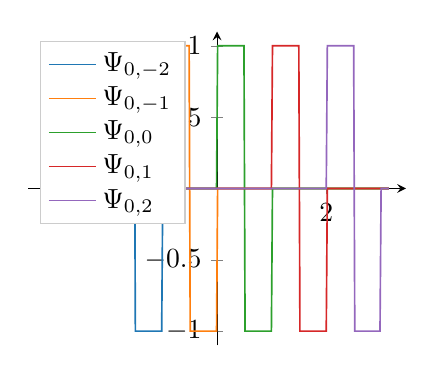
\begin{tikzpicture}

\definecolor{color0}{rgb}{0.12156862745098,0.466666666666667,0.705882352941177}
\definecolor{color1}{rgb}{1,0.498039215686275,0.0549019607843137}
\definecolor{color2}{rgb}{0.172549019607843,0.627450980392157,0.172549019607843}
\definecolor{color3}{rgb}{0.83921568627451,0.152941176470588,0.156862745098039}
\definecolor{color4}{rgb}{0.580392156862745,0.403921568627451,0.741176470588235}

\begin{axis}[
axis x line=center,
axis y line=center,
xmin=-3.45575191894877, xmax=3.45575191894877,
ymin=-1.1, ymax=1.1,
x grid style={white!69.01960784313725!black},
y grid style={white!69.01960784313725!black},
legend entries={{$\Psi_{0,-2}$},{$\Psi_{0,-1}$},{$\Psi_{0,0}$},{$\Psi_{0,1}$},{$\Psi_{0,2}$}},
legend cell align={left},
legend style={at={(0.03,0.97)}, anchor=north west, draw=white!80.0!black},
scale=.7
]
\addlegendimage{no markers, color0}
\addlegendimage{no markers, color1}
\addlegendimage{no markers, color2}
\addlegendimage{no markers, color3}
\addlegendimage{no markers, color4}
\addplot [semithick, color0]
table {%
-3.14159265358979 0
-3.12151857912596 0
-3.10144450466213 0
-3.0813704301983 0
-3.06129635573446 0
-3.04122228127063 0
-3.0211482068068 0
-3.00107413234297 0
-2.98100005787913 0
-2.9609259834153 0
-2.94085190895147 0
-2.92077783448764 0
-2.9007037600238 0
-2.88062968555997 0
-2.86055561109614 0
-2.8404815366323 0
-2.82040746216847 0
-2.80033338770464 0
-2.78025931324081 0
-2.76018523877697 0
-2.74011116431314 0
-2.72003708984931 0
-2.69996301538548 0
-2.67988894092164 0
-2.65981486645781 0
-2.63974079199398 0
-2.61966671753015 0
-2.59959264306631 0
-2.57951856860248 0
-2.55944449413865 0
-2.53937041967482 0
-2.51929634521098 0
-2.49922227074715 0
-2.47914819628332 0
-2.45907412181949 0
-2.43900004735565 0
-2.41892597289182 0
-2.39885189842799 0
-2.37877782396416 0
-2.35870374950032 0
-2.33862967503649 0
-2.31855560057266 0
-2.29848152610883 0
-2.27840745164499 0
-2.25833337718116 0
-2.23825930271733 0
-2.2181852282535 0
-2.19811115378966 0
-2.17803707932583 0
-2.157963004862 0
-2.13788893039817 0
-2.11781485593433 0
-2.0977407814705 0
-2.07766670700667 0
-2.05759263254284 0
-2.037518558079 0
-2.01744448361517 0
-1.99737040915134 1
-1.97729633468751 1
-1.95722226022367 1
-1.93714818575984 1
-1.91707411129601 1
-1.89700003683218 1
-1.87692596236834 1
-1.85685188790451 1
-1.83677781344068 1
-1.81670373897685 1
-1.79662966451301 1
-1.77655559004918 1
-1.75648151558535 1
-1.73640744112152 1
-1.71633336665768 1
-1.69625929219385 1
-1.67618521773002 1
-1.65611114326619 1
-1.63603706880235 1
-1.61596299433852 1
-1.59588891987469 1
-1.57581484541085 1
-1.55574077094702 1
-1.53566669648319 1
-1.51559262201936 1
-1.49551854755552 -1
-1.47544447309169 -1
-1.45537039862786 -1
-1.43529632416403 -1
-1.41522224970019 -1
-1.39514817523636 -1
-1.37507410077253 -1
-1.3550000263087 -1
-1.33492595184486 -1
-1.31485187738103 -1
-1.2947778029172 -1
-1.27470372845337 -1
-1.25462965398953 -1
-1.2345555795257 -1
-1.21448150506187 -1
-1.19440743059804 -1
-1.1743333561342 -1
-1.15425928167037 -1
-1.13418520720654 -1
-1.11411113274271 -1
-1.09403705827887 -1
-1.07396298381504 -1
-1.05388890935121 -1
-1.03381483488738 -1
-1.01374076042354 -1
-0.993666685959711 0
-0.973592611495878 0
-0.953518537032046 0
-0.933444462568213 0
-0.913370388104381 0
-0.893296313640549 0
-0.873222239176716 0
-0.853148164712883 0
-0.833074090249051 0
-0.813000015785218 0
-0.792925941321386 0
-0.772851866857553 0
-0.75277779239372 0
-0.732703717929888 0
-0.712629643466055 0
-0.692555569002223 0
-0.672481494538391 0
-0.652407420074558 0
-0.632333345610725 0
-0.612259271146893 0
-0.59218519668306 0
-0.572111122219228 0
-0.552037047755395 0
-0.531962973291563 0
-0.51188889882773 0
-0.491814824363897 0
-0.471740749900065 0
-0.451666675436233 0
-0.4315926009724 0
-0.411518526508567 0
-0.391444452044735 0
-0.371370377580902 0
-0.35129630311707 0
-0.331222228653237 0
-0.311148154189405 0
-0.291074079725572 0
-0.271000005261739 0
-0.250925930797907 0
-0.230851856334074 0
-0.210777781870242 0
-0.19070370740641 0
-0.170629632942577 0
-0.150555558478744 0
-0.130481484014912 0
-0.110407409551079 0
-0.0903333350872466 0
-0.070259260623414 0
-0.0501851861595815 0
-0.0301111116957489 0
-0.0100370372319163 0
0.0100370372319163 0
0.0301111116957484 0
0.050185186159581 0
0.0702592606234136 0
0.0903333350872462 0
0.110407409551079 0
0.130481484014911 0
0.150555558478744 0
0.170629632942576 0
0.190703707406409 0
0.210777781870242 0
0.230851856334074 0
0.250925930797906 0
0.271000005261739 0
0.291074079725572 0
0.311148154189404 0
0.331222228653237 0
0.351296303117069 0
0.371370377580902 0
0.391444452044734 0
0.411518526508567 0
0.4315926009724 0
0.451666675436232 0
0.471740749900065 0
0.491814824363897 0
0.511888898827729 0
0.531962973291562 0
0.552037047755395 0
0.572111122219227 0
0.59218519668306 0
0.612259271146892 0
0.632333345610725 0
0.652407420074558 0
0.67248149453839 0
0.692555569002223 0
0.712629643466055 0
0.732703717929887 0
0.75277779239372 0
0.772851866857553 0
0.792925941321385 0
0.813000015785218 0
0.83307409024905 0
0.853148164712883 0
0.873222239176715 0
0.893296313640548 0
0.91337038810438 0
0.933444462568213 0
0.953518537032045 0
0.973592611495878 0
0.993666685959711 0
1.01374076042354 0
1.03381483488738 0
1.05388890935121 0
1.07396298381504 0
1.09403705827887 0
1.11411113274271 0
1.13418520720654 0
1.15425928167037 0
1.1743333561342 0
1.19440743059804 0
1.21448150506187 0
1.2345555795257 0
1.25462965398953 0
1.27470372845337 0
1.2947778029172 0
1.31485187738103 0
1.33492595184486 0
1.3550000263087 0
1.37507410077253 0
1.39514817523636 0
1.41522224970019 0
1.43529632416403 0
1.45537039862786 0
1.47544447309169 0
1.49551854755552 0
1.51559262201936 0
1.53566669648319 0
1.55574077094702 0
1.57581484541085 0
1.59588891987469 0
1.61596299433852 0
1.63603706880235 0
1.65611114326618 0
1.67618521773002 0
1.69625929219385 0
1.71633336665768 0
1.73640744112152 0
1.75648151558535 0
1.77655559004918 0
1.79662966451301 0
1.81670373897684 0
1.83677781344068 0
1.85685188790451 0
1.87692596236834 0
1.89700003683217 0
1.91707411129601 0
1.93714818575984 0
1.95722226022367 0
1.97729633468751 0
1.99737040915134 0
2.01744448361517 0
2.037518558079 0
2.05759263254284 0
2.07766670700667 0
2.0977407814705 0
2.11781485593433 0
2.13788893039817 0
2.157963004862 0
2.17803707932583 0
2.19811115378966 0
2.2181852282535 0
2.23825930271733 0
2.25833337718116 0
2.27840745164499 0
2.29848152610883 0
2.31855560057266 0
2.33862967503649 0
2.35870374950032 0
2.37877782396416 0
2.39885189842799 0
2.41892597289182 0
2.43900004735565 0
2.45907412181949 0
2.47914819628332 0
2.49922227074715 0
2.51929634521098 0
2.53937041967482 0
2.55944449413865 0
2.57951856860248 0
2.59959264306631 0
2.61966671753015 0
2.63974079199398 0
2.65981486645781 0
2.67988894092164 0
2.69996301538548 0
2.72003708984931 0
2.74011116431314 0
2.76018523877697 0
2.78025931324081 0
2.80033338770464 0
2.82040746216847 0
2.8404815366323 0
2.86055561109614 0
2.88062968555997 0
2.9007037600238 0
2.92077783448763 0
2.94085190895147 0
2.9609259834153 0
2.98100005787913 0
3.00107413234297 0
3.0211482068068 0
3.04122228127063 0
3.06129635573446 0
3.0813704301983 0
3.10144450466213 0
3.12151857912596 0
3.14159265358979 0
};
\addplot [semithick, color1]
table {%
-3.14159265358979 0
-3.12151857912596 0
-3.10144450466213 0
-3.0813704301983 0
-3.06129635573446 0
-3.04122228127063 0
-3.0211482068068 0
-3.00107413234297 0
-2.98100005787913 0
-2.9609259834153 0
-2.94085190895147 0
-2.92077783448764 0
-2.9007037600238 0
-2.88062968555997 0
-2.86055561109614 0
-2.8404815366323 0
-2.82040746216847 0
-2.80033338770464 0
-2.78025931324081 0
-2.76018523877697 0
-2.74011116431314 0
-2.72003708984931 0
-2.69996301538548 0
-2.67988894092164 0
-2.65981486645781 0
-2.63974079199398 0
-2.61966671753015 0
-2.59959264306631 0
-2.57951856860248 0
-2.55944449413865 0
-2.53937041967482 0
-2.51929634521098 0
-2.49922227074715 0
-2.47914819628332 0
-2.45907412181949 0
-2.43900004735565 0
-2.41892597289182 0
-2.39885189842799 0
-2.37877782396416 0
-2.35870374950032 0
-2.33862967503649 0
-2.31855560057266 0
-2.29848152610883 0
-2.27840745164499 0
-2.25833337718116 0
-2.23825930271733 0
-2.2181852282535 0
-2.19811115378966 0
-2.17803707932583 0
-2.157963004862 0
-2.13788893039817 0
-2.11781485593433 0
-2.0977407814705 0
-2.07766670700667 0
-2.05759263254284 0
-2.037518558079 0
-2.01744448361517 0
-1.99737040915134 0
-1.97729633468751 0
-1.95722226022367 0
-1.93714818575984 0
-1.91707411129601 0
-1.89700003683218 0
-1.87692596236834 0
-1.85685188790451 0
-1.83677781344068 0
-1.81670373897685 0
-1.79662966451301 0
-1.77655559004918 0
-1.75648151558535 0
-1.73640744112152 0
-1.71633336665768 0
-1.69625929219385 0
-1.67618521773002 0
-1.65611114326619 0
-1.63603706880235 0
-1.61596299433852 0
-1.59588891987469 0
-1.57581484541085 0
-1.55574077094702 0
-1.53566669648319 0
-1.51559262201936 0
-1.49551854755552 0
-1.47544447309169 0
-1.45537039862786 0
-1.43529632416403 0
-1.41522224970019 0
-1.39514817523636 0
-1.37507410077253 0
-1.3550000263087 0
-1.33492595184486 0
-1.31485187738103 0
-1.2947778029172 0
-1.27470372845337 0
-1.25462965398953 0
-1.2345555795257 0
-1.21448150506187 0
-1.19440743059804 0
-1.1743333561342 0
-1.15425928167037 0
-1.13418520720654 0
-1.11411113274271 0
-1.09403705827887 0
-1.07396298381504 0
-1.05388890935121 0
-1.03381483488738 0
-1.01374076042354 0
-0.993666685959711 1
-0.973592611495878 1
-0.953518537032046 1
-0.933444462568213 1
-0.913370388104381 1
-0.893296313640549 1
-0.873222239176716 1
-0.853148164712883 1
-0.833074090249051 1
-0.813000015785218 1
-0.792925941321386 1
-0.772851866857553 1
-0.75277779239372 1
-0.732703717929888 1
-0.712629643466055 1
-0.692555569002223 1
-0.672481494538391 1
-0.652407420074558 1
-0.632333345610725 1
-0.612259271146893 1
-0.59218519668306 1
-0.572111122219228 1
-0.552037047755395 1
-0.531962973291563 1
-0.51188889882773 1
-0.491814824363897 -1
-0.471740749900065 -1
-0.451666675436233 -1
-0.4315926009724 -1
-0.411518526508567 -1
-0.391444452044735 -1
-0.371370377580902 -1
-0.35129630311707 -1
-0.331222228653237 -1
-0.311148154189405 -1
-0.291074079725572 -1
-0.271000005261739 -1
-0.250925930797907 -1
-0.230851856334074 -1
-0.210777781870242 -1
-0.19070370740641 -1
-0.170629632942577 -1
-0.150555558478744 -1
-0.130481484014912 -1
-0.110407409551079 -1
-0.0903333350872466 -1
-0.070259260623414 -1
-0.0501851861595815 -1
-0.0301111116957489 -1
-0.0100370372319163 -1
0.0100370372319163 0
0.0301111116957484 0
0.050185186159581 0
0.0702592606234136 0
0.0903333350872462 0
0.110407409551079 0
0.130481484014911 0
0.150555558478744 0
0.170629632942576 0
0.190703707406409 0
0.210777781870242 0
0.230851856334074 0
0.250925930797906 0
0.271000005261739 0
0.291074079725572 0
0.311148154189404 0
0.331222228653237 0
0.351296303117069 0
0.371370377580902 0
0.391444452044734 0
0.411518526508567 0
0.4315926009724 0
0.451666675436232 0
0.471740749900065 0
0.491814824363897 0
0.511888898827729 0
0.531962973291562 0
0.552037047755395 0
0.572111122219227 0
0.59218519668306 0
0.612259271146892 0
0.632333345610725 0
0.652407420074558 0
0.67248149453839 0
0.692555569002223 0
0.712629643466055 0
0.732703717929887 0
0.75277779239372 0
0.772851866857553 0
0.792925941321385 0
0.813000015785218 0
0.83307409024905 0
0.853148164712883 0
0.873222239176715 0
0.893296313640548 0
0.91337038810438 0
0.933444462568213 0
0.953518537032045 0
0.973592611495878 0
0.993666685959711 0
1.01374076042354 0
1.03381483488738 0
1.05388890935121 0
1.07396298381504 0
1.09403705827887 0
1.11411113274271 0
1.13418520720654 0
1.15425928167037 0
1.1743333561342 0
1.19440743059804 0
1.21448150506187 0
1.2345555795257 0
1.25462965398953 0
1.27470372845337 0
1.2947778029172 0
1.31485187738103 0
1.33492595184486 0
1.3550000263087 0
1.37507410077253 0
1.39514817523636 0
1.41522224970019 0
1.43529632416403 0
1.45537039862786 0
1.47544447309169 0
1.49551854755552 0
1.51559262201936 0
1.53566669648319 0
1.55574077094702 0
1.57581484541085 0
1.59588891987469 0
1.61596299433852 0
1.63603706880235 0
1.65611114326618 0
1.67618521773002 0
1.69625929219385 0
1.71633336665768 0
1.73640744112152 0
1.75648151558535 0
1.77655559004918 0
1.79662966451301 0
1.81670373897684 0
1.83677781344068 0
1.85685188790451 0
1.87692596236834 0
1.89700003683217 0
1.91707411129601 0
1.93714818575984 0
1.95722226022367 0
1.97729633468751 0
1.99737040915134 0
2.01744448361517 0
2.037518558079 0
2.05759263254284 0
2.07766670700667 0
2.0977407814705 0
2.11781485593433 0
2.13788893039817 0
2.157963004862 0
2.17803707932583 0
2.19811115378966 0
2.2181852282535 0
2.23825930271733 0
2.25833337718116 0
2.27840745164499 0
2.29848152610883 0
2.31855560057266 0
2.33862967503649 0
2.35870374950032 0
2.37877782396416 0
2.39885189842799 0
2.41892597289182 0
2.43900004735565 0
2.45907412181949 0
2.47914819628332 0
2.49922227074715 0
2.51929634521098 0
2.53937041967482 0
2.55944449413865 0
2.57951856860248 0
2.59959264306631 0
2.61966671753015 0
2.63974079199398 0
2.65981486645781 0
2.67988894092164 0
2.69996301538548 0
2.72003708984931 0
2.74011116431314 0
2.76018523877697 0
2.78025931324081 0
2.80033338770464 0
2.82040746216847 0
2.8404815366323 0
2.86055561109614 0
2.88062968555997 0
2.9007037600238 0
2.92077783448763 0
2.94085190895147 0
2.9609259834153 0
2.98100005787913 0
3.00107413234297 0
3.0211482068068 0
3.04122228127063 0
3.06129635573446 0
3.0813704301983 0
3.10144450466213 0
3.12151857912596 0
3.14159265358979 0
};
\addplot [semithick, color2]
table {%
-3.14159265358979 0
-3.12151857912596 0
-3.10144450466213 0
-3.0813704301983 0
-3.06129635573446 0
-3.04122228127063 0
-3.0211482068068 0
-3.00107413234297 0
-2.98100005787913 0
-2.9609259834153 0
-2.94085190895147 0
-2.92077783448764 0
-2.9007037600238 0
-2.88062968555997 0
-2.86055561109614 0
-2.8404815366323 0
-2.82040746216847 0
-2.80033338770464 0
-2.78025931324081 0
-2.76018523877697 0
-2.74011116431314 0
-2.72003708984931 0
-2.69996301538548 0
-2.67988894092164 0
-2.65981486645781 0
-2.63974079199398 0
-2.61966671753015 0
-2.59959264306631 0
-2.57951856860248 0
-2.55944449413865 0
-2.53937041967482 0
-2.51929634521098 0
-2.49922227074715 0
-2.47914819628332 0
-2.45907412181949 0
-2.43900004735565 0
-2.41892597289182 0
-2.39885189842799 0
-2.37877782396416 0
-2.35870374950032 0
-2.33862967503649 0
-2.31855560057266 0
-2.29848152610883 0
-2.27840745164499 0
-2.25833337718116 0
-2.23825930271733 0
-2.2181852282535 0
-2.19811115378966 0
-2.17803707932583 0
-2.157963004862 0
-2.13788893039817 0
-2.11781485593433 0
-2.0977407814705 0
-2.07766670700667 0
-2.05759263254284 0
-2.037518558079 0
-2.01744448361517 0
-1.99737040915134 0
-1.97729633468751 0
-1.95722226022367 0
-1.93714818575984 0
-1.91707411129601 0
-1.89700003683218 0
-1.87692596236834 0
-1.85685188790451 0
-1.83677781344068 0
-1.81670373897685 0
-1.79662966451301 0
-1.77655559004918 0
-1.75648151558535 0
-1.73640744112152 0
-1.71633336665768 0
-1.69625929219385 0
-1.67618521773002 0
-1.65611114326619 0
-1.63603706880235 0
-1.61596299433852 0
-1.59588891987469 0
-1.57581484541085 0
-1.55574077094702 0
-1.53566669648319 0
-1.51559262201936 0
-1.49551854755552 0
-1.47544447309169 0
-1.45537039862786 0
-1.43529632416403 0
-1.41522224970019 0
-1.39514817523636 0
-1.37507410077253 0
-1.3550000263087 0
-1.33492595184486 0
-1.31485187738103 0
-1.2947778029172 0
-1.27470372845337 0
-1.25462965398953 0
-1.2345555795257 0
-1.21448150506187 0
-1.19440743059804 0
-1.1743333561342 0
-1.15425928167037 0
-1.13418520720654 0
-1.11411113274271 0
-1.09403705827887 0
-1.07396298381504 0
-1.05388890935121 0
-1.03381483488738 0
-1.01374076042354 0
-0.993666685959711 0
-0.973592611495878 0
-0.953518537032046 0
-0.933444462568213 0
-0.913370388104381 0
-0.893296313640549 0
-0.873222239176716 0
-0.853148164712883 0
-0.833074090249051 0
-0.813000015785218 0
-0.792925941321386 0
-0.772851866857553 0
-0.75277779239372 0
-0.732703717929888 0
-0.712629643466055 0
-0.692555569002223 0
-0.672481494538391 0
-0.652407420074558 0
-0.632333345610725 0
-0.612259271146893 0
-0.59218519668306 0
-0.572111122219228 0
-0.552037047755395 0
-0.531962973291563 0
-0.51188889882773 0
-0.491814824363897 0
-0.471740749900065 0
-0.451666675436233 0
-0.4315926009724 0
-0.411518526508567 0
-0.391444452044735 0
-0.371370377580902 0
-0.35129630311707 0
-0.331222228653237 0
-0.311148154189405 0
-0.291074079725572 0
-0.271000005261739 0
-0.250925930797907 0
-0.230851856334074 0
-0.210777781870242 0
-0.19070370740641 0
-0.170629632942577 0
-0.150555558478744 0
-0.130481484014912 0
-0.110407409551079 0
-0.0903333350872466 0
-0.070259260623414 0
-0.0501851861595815 0
-0.0301111116957489 0
-0.0100370372319163 0
0.0100370372319163 1
0.0301111116957484 1
0.050185186159581 1
0.0702592606234136 1
0.0903333350872462 1
0.110407409551079 1
0.130481484014911 1
0.150555558478744 1
0.170629632942576 1
0.190703707406409 1
0.210777781870242 1
0.230851856334074 1
0.250925930797906 1
0.271000005261739 1
0.291074079725572 1
0.311148154189404 1
0.331222228653237 1
0.351296303117069 1
0.371370377580902 1
0.391444452044734 1
0.411518526508567 1
0.4315926009724 1
0.451666675436232 1
0.471740749900065 1
0.491814824363897 1
0.511888898827729 -1
0.531962973291562 -1
0.552037047755395 -1
0.572111122219227 -1
0.59218519668306 -1
0.612259271146892 -1
0.632333345610725 -1
0.652407420074558 -1
0.67248149453839 -1
0.692555569002223 -1
0.712629643466055 -1
0.732703717929887 -1
0.75277779239372 -1
0.772851866857553 -1
0.792925941321385 -1
0.813000015785218 -1
0.83307409024905 -1
0.853148164712883 -1
0.873222239176715 -1
0.893296313640548 -1
0.91337038810438 -1
0.933444462568213 -1
0.953518537032045 -1
0.973592611495878 -1
0.993666685959711 -1
1.01374076042354 0
1.03381483488738 0
1.05388890935121 0
1.07396298381504 0
1.09403705827887 0
1.11411113274271 0
1.13418520720654 0
1.15425928167037 0
1.1743333561342 0
1.19440743059804 0
1.21448150506187 0
1.2345555795257 0
1.25462965398953 0
1.27470372845337 0
1.2947778029172 0
1.31485187738103 0
1.33492595184486 0
1.3550000263087 0
1.37507410077253 0
1.39514817523636 0
1.41522224970019 0
1.43529632416403 0
1.45537039862786 0
1.47544447309169 0
1.49551854755552 0
1.51559262201936 0
1.53566669648319 0
1.55574077094702 0
1.57581484541085 0
1.59588891987469 0
1.61596299433852 0
1.63603706880235 0
1.65611114326618 0
1.67618521773002 0
1.69625929219385 0
1.71633336665768 0
1.73640744112152 0
1.75648151558535 0
1.77655559004918 0
1.79662966451301 0
1.81670373897684 0
1.83677781344068 0
1.85685188790451 0
1.87692596236834 0
1.89700003683217 0
1.91707411129601 0
1.93714818575984 0
1.95722226022367 0
1.97729633468751 0
1.99737040915134 0
2.01744448361517 0
2.037518558079 0
2.05759263254284 0
2.07766670700667 0
2.0977407814705 0
2.11781485593433 0
2.13788893039817 0
2.157963004862 0
2.17803707932583 0
2.19811115378966 0
2.2181852282535 0
2.23825930271733 0
2.25833337718116 0
2.27840745164499 0
2.29848152610883 0
2.31855560057266 0
2.33862967503649 0
2.35870374950032 0
2.37877782396416 0
2.39885189842799 0
2.41892597289182 0
2.43900004735565 0
2.45907412181949 0
2.47914819628332 0
2.49922227074715 0
2.51929634521098 0
2.53937041967482 0
2.55944449413865 0
2.57951856860248 0
2.59959264306631 0
2.61966671753015 0
2.63974079199398 0
2.65981486645781 0
2.67988894092164 0
2.69996301538548 0
2.72003708984931 0
2.74011116431314 0
2.76018523877697 0
2.78025931324081 0
2.80033338770464 0
2.82040746216847 0
2.8404815366323 0
2.86055561109614 0
2.88062968555997 0
2.9007037600238 0
2.92077783448763 0
2.94085190895147 0
2.9609259834153 0
2.98100005787913 0
3.00107413234297 0
3.0211482068068 0
3.04122228127063 0
3.06129635573446 0
3.0813704301983 0
3.10144450466213 0
3.12151857912596 0
3.14159265358979 0
};
\addplot [semithick, color3]
table {%
-3.14159265358979 0
-3.12151857912596 0
-3.10144450466213 0
-3.0813704301983 0
-3.06129635573446 0
-3.04122228127063 0
-3.0211482068068 0
-3.00107413234297 0
-2.98100005787913 0
-2.9609259834153 0
-2.94085190895147 0
-2.92077783448764 0
-2.9007037600238 0
-2.88062968555997 0
-2.86055561109614 0
-2.8404815366323 0
-2.82040746216847 0
-2.80033338770464 0
-2.78025931324081 0
-2.76018523877697 0
-2.74011116431314 0
-2.72003708984931 0
-2.69996301538548 0
-2.67988894092164 0
-2.65981486645781 0
-2.63974079199398 0
-2.61966671753015 0
-2.59959264306631 0
-2.57951856860248 0
-2.55944449413865 0
-2.53937041967482 0
-2.51929634521098 0
-2.49922227074715 0
-2.47914819628332 0
-2.45907412181949 0
-2.43900004735565 0
-2.41892597289182 0
-2.39885189842799 0
-2.37877782396416 0
-2.35870374950032 0
-2.33862967503649 0
-2.31855560057266 0
-2.29848152610883 0
-2.27840745164499 0
-2.25833337718116 0
-2.23825930271733 0
-2.2181852282535 0
-2.19811115378966 0
-2.17803707932583 0
-2.157963004862 0
-2.13788893039817 0
-2.11781485593433 0
-2.0977407814705 0
-2.07766670700667 0
-2.05759263254284 0
-2.037518558079 0
-2.01744448361517 0
-1.99737040915134 0
-1.97729633468751 0
-1.95722226022367 0
-1.93714818575984 0
-1.91707411129601 0
-1.89700003683218 0
-1.87692596236834 0
-1.85685188790451 0
-1.83677781344068 0
-1.81670373897685 0
-1.79662966451301 0
-1.77655559004918 0
-1.75648151558535 0
-1.73640744112152 0
-1.71633336665768 0
-1.69625929219385 0
-1.67618521773002 0
-1.65611114326619 0
-1.63603706880235 0
-1.61596299433852 0
-1.59588891987469 0
-1.57581484541085 0
-1.55574077094702 0
-1.53566669648319 0
-1.51559262201936 0
-1.49551854755552 0
-1.47544447309169 0
-1.45537039862786 0
-1.43529632416403 0
-1.41522224970019 0
-1.39514817523636 0
-1.37507410077253 0
-1.3550000263087 0
-1.33492595184486 0
-1.31485187738103 0
-1.2947778029172 0
-1.27470372845337 0
-1.25462965398953 0
-1.2345555795257 0
-1.21448150506187 0
-1.19440743059804 0
-1.1743333561342 0
-1.15425928167037 0
-1.13418520720654 0
-1.11411113274271 0
-1.09403705827887 0
-1.07396298381504 0
-1.05388890935121 0
-1.03381483488738 0
-1.01374076042354 0
-0.993666685959711 0
-0.973592611495878 0
-0.953518537032046 0
-0.933444462568213 0
-0.913370388104381 0
-0.893296313640549 0
-0.873222239176716 0
-0.853148164712883 0
-0.833074090249051 0
-0.813000015785218 0
-0.792925941321386 0
-0.772851866857553 0
-0.75277779239372 0
-0.732703717929888 0
-0.712629643466055 0
-0.692555569002223 0
-0.672481494538391 0
-0.652407420074558 0
-0.632333345610725 0
-0.612259271146893 0
-0.59218519668306 0
-0.572111122219228 0
-0.552037047755395 0
-0.531962973291563 0
-0.51188889882773 0
-0.491814824363897 0
-0.471740749900065 0
-0.451666675436233 0
-0.4315926009724 0
-0.411518526508567 0
-0.391444452044735 0
-0.371370377580902 0
-0.35129630311707 0
-0.331222228653237 0
-0.311148154189405 0
-0.291074079725572 0
-0.271000005261739 0
-0.250925930797907 0
-0.230851856334074 0
-0.210777781870242 0
-0.19070370740641 0
-0.170629632942577 0
-0.150555558478744 0
-0.130481484014912 0
-0.110407409551079 0
-0.0903333350872466 0
-0.070259260623414 0
-0.0501851861595815 0
-0.0301111116957489 0
-0.0100370372319163 0
0.0100370372319163 0
0.0301111116957484 0
0.050185186159581 0
0.0702592606234136 0
0.0903333350872462 0
0.110407409551079 0
0.130481484014911 0
0.150555558478744 0
0.170629632942576 0
0.190703707406409 0
0.210777781870242 0
0.230851856334074 0
0.250925930797906 0
0.271000005261739 0
0.291074079725572 0
0.311148154189404 0
0.331222228653237 0
0.351296303117069 0
0.371370377580902 0
0.391444452044734 0
0.411518526508567 0
0.4315926009724 0
0.451666675436232 0
0.471740749900065 0
0.491814824363897 0
0.511888898827729 0
0.531962973291562 0
0.552037047755395 0
0.572111122219227 0
0.59218519668306 0
0.612259271146892 0
0.632333345610725 0
0.652407420074558 0
0.67248149453839 0
0.692555569002223 0
0.712629643466055 0
0.732703717929887 0
0.75277779239372 0
0.772851866857553 0
0.792925941321385 0
0.813000015785218 0
0.83307409024905 0
0.853148164712883 0
0.873222239176715 0
0.893296313640548 0
0.91337038810438 0
0.933444462568213 0
0.953518537032045 0
0.973592611495878 0
0.993666685959711 0
1.01374076042354 1
1.03381483488738 1
1.05388890935121 1
1.07396298381504 1
1.09403705827887 1
1.11411113274271 1
1.13418520720654 1
1.15425928167037 1
1.1743333561342 1
1.19440743059804 1
1.21448150506187 1
1.2345555795257 1
1.25462965398953 1
1.27470372845337 1
1.2947778029172 1
1.31485187738103 1
1.33492595184486 1
1.3550000263087 1
1.37507410077253 1
1.39514817523636 1
1.41522224970019 1
1.43529632416403 1
1.45537039862786 1
1.47544447309169 1
1.49551854755552 1
1.51559262201936 -1
1.53566669648319 -1
1.55574077094702 -1
1.57581484541085 -1
1.59588891987469 -1
1.61596299433852 -1
1.63603706880235 -1
1.65611114326618 -1
1.67618521773002 -1
1.69625929219385 -1
1.71633336665768 -1
1.73640744112152 -1
1.75648151558535 -1
1.77655559004918 -1
1.79662966451301 -1
1.81670373897684 -1
1.83677781344068 -1
1.85685188790451 -1
1.87692596236834 -1
1.89700003683217 -1
1.91707411129601 -1
1.93714818575984 -1
1.95722226022367 -1
1.97729633468751 -1
1.99737040915134 -1
2.01744448361517 0
2.037518558079 0
2.05759263254284 0
2.07766670700667 0
2.0977407814705 0
2.11781485593433 0
2.13788893039817 0
2.157963004862 0
2.17803707932583 0
2.19811115378966 0
2.2181852282535 0
2.23825930271733 0
2.25833337718116 0
2.27840745164499 0
2.29848152610883 0
2.31855560057266 0
2.33862967503649 0
2.35870374950032 0
2.37877782396416 0
2.39885189842799 0
2.41892597289182 0
2.43900004735565 0
2.45907412181949 0
2.47914819628332 0
2.49922227074715 0
2.51929634521098 0
2.53937041967482 0
2.55944449413865 0
2.57951856860248 0
2.59959264306631 0
2.61966671753015 0
2.63974079199398 0
2.65981486645781 0
2.67988894092164 0
2.69996301538548 0
2.72003708984931 0
2.74011116431314 0
2.76018523877697 0
2.78025931324081 0
2.80033338770464 0
2.82040746216847 0
2.8404815366323 0
2.86055561109614 0
2.88062968555997 0
2.9007037600238 0
2.92077783448763 0
2.94085190895147 0
2.9609259834153 0
2.98100005787913 0
3.00107413234297 0
3.0211482068068 0
3.04122228127063 0
3.06129635573446 0
3.0813704301983 0
3.10144450466213 0
3.12151857912596 0
3.14159265358979 0
};
\addplot [semithick, color4]
table {%
-3.14159265358979 0
-3.12151857912596 0
-3.10144450466213 0
-3.0813704301983 0
-3.06129635573446 0
-3.04122228127063 0
-3.0211482068068 0
-3.00107413234297 0
-2.98100005787913 0
-2.9609259834153 0
-2.94085190895147 0
-2.92077783448764 0
-2.9007037600238 0
-2.88062968555997 0
-2.86055561109614 0
-2.8404815366323 0
-2.82040746216847 0
-2.80033338770464 0
-2.78025931324081 0
-2.76018523877697 0
-2.74011116431314 0
-2.72003708984931 0
-2.69996301538548 0
-2.67988894092164 0
-2.65981486645781 0
-2.63974079199398 0
-2.61966671753015 0
-2.59959264306631 0
-2.57951856860248 0
-2.55944449413865 0
-2.53937041967482 0
-2.51929634521098 0
-2.49922227074715 0
-2.47914819628332 0
-2.45907412181949 0
-2.43900004735565 0
-2.41892597289182 0
-2.39885189842799 0
-2.37877782396416 0
-2.35870374950032 0
-2.33862967503649 0
-2.31855560057266 0
-2.29848152610883 0
-2.27840745164499 0
-2.25833337718116 0
-2.23825930271733 0
-2.2181852282535 0
-2.19811115378966 0
-2.17803707932583 0
-2.157963004862 0
-2.13788893039817 0
-2.11781485593433 0
-2.0977407814705 0
-2.07766670700667 0
-2.05759263254284 0
-2.037518558079 0
-2.01744448361517 0
-1.99737040915134 0
-1.97729633468751 0
-1.95722226022367 0
-1.93714818575984 0
-1.91707411129601 0
-1.89700003683218 0
-1.87692596236834 0
-1.85685188790451 0
-1.83677781344068 0
-1.81670373897685 0
-1.79662966451301 0
-1.77655559004918 0
-1.75648151558535 0
-1.73640744112152 0
-1.71633336665768 0
-1.69625929219385 0
-1.67618521773002 0
-1.65611114326619 0
-1.63603706880235 0
-1.61596299433852 0
-1.59588891987469 0
-1.57581484541085 0
-1.55574077094702 0
-1.53566669648319 0
-1.51559262201936 0
-1.49551854755552 0
-1.47544447309169 0
-1.45537039862786 0
-1.43529632416403 0
-1.41522224970019 0
-1.39514817523636 0
-1.37507410077253 0
-1.3550000263087 0
-1.33492595184486 0
-1.31485187738103 0
-1.2947778029172 0
-1.27470372845337 0
-1.25462965398953 0
-1.2345555795257 0
-1.21448150506187 0
-1.19440743059804 0
-1.1743333561342 0
-1.15425928167037 0
-1.13418520720654 0
-1.11411113274271 0
-1.09403705827887 0
-1.07396298381504 0
-1.05388890935121 0
-1.03381483488738 0
-1.01374076042354 0
-0.993666685959711 0
-0.973592611495878 0
-0.953518537032046 0
-0.933444462568213 0
-0.913370388104381 0
-0.893296313640549 0
-0.873222239176716 0
-0.853148164712883 0
-0.833074090249051 0
-0.813000015785218 0
-0.792925941321386 0
-0.772851866857553 0
-0.75277779239372 0
-0.732703717929888 0
-0.712629643466055 0
-0.692555569002223 0
-0.672481494538391 0
-0.652407420074558 0
-0.632333345610725 0
-0.612259271146893 0
-0.59218519668306 0
-0.572111122219228 0
-0.552037047755395 0
-0.531962973291563 0
-0.51188889882773 0
-0.491814824363897 0
-0.471740749900065 0
-0.451666675436233 0
-0.4315926009724 0
-0.411518526508567 0
-0.391444452044735 0
-0.371370377580902 0
-0.35129630311707 0
-0.331222228653237 0
-0.311148154189405 0
-0.291074079725572 0
-0.271000005261739 0
-0.250925930797907 0
-0.230851856334074 0
-0.210777781870242 0
-0.19070370740641 0
-0.170629632942577 0
-0.150555558478744 0
-0.130481484014912 0
-0.110407409551079 0
-0.0903333350872466 0
-0.070259260623414 0
-0.0501851861595815 0
-0.0301111116957489 0
-0.0100370372319163 0
0.0100370372319163 0
0.0301111116957484 0
0.050185186159581 0
0.0702592606234136 0
0.0903333350872462 0
0.110407409551079 0
0.130481484014911 0
0.150555558478744 0
0.170629632942576 0
0.190703707406409 0
0.210777781870242 0
0.230851856334074 0
0.250925930797906 0
0.271000005261739 0
0.291074079725572 0
0.311148154189404 0
0.331222228653237 0
0.351296303117069 0
0.371370377580902 0
0.391444452044734 0
0.411518526508567 0
0.4315926009724 0
0.451666675436232 0
0.471740749900065 0
0.491814824363897 0
0.511888898827729 0
0.531962973291562 0
0.552037047755395 0
0.572111122219227 0
0.59218519668306 0
0.612259271146892 0
0.632333345610725 0
0.652407420074558 0
0.67248149453839 0
0.692555569002223 0
0.712629643466055 0
0.732703717929887 0
0.75277779239372 0
0.772851866857553 0
0.792925941321385 0
0.813000015785218 0
0.83307409024905 0
0.853148164712883 0
0.873222239176715 0
0.893296313640548 0
0.91337038810438 0
0.933444462568213 0
0.953518537032045 0
0.973592611495878 0
0.993666685959711 0
1.01374076042354 0
1.03381483488738 0
1.05388890935121 0
1.07396298381504 0
1.09403705827887 0
1.11411113274271 0
1.13418520720654 0
1.15425928167037 0
1.1743333561342 0
1.19440743059804 0
1.21448150506187 0
1.2345555795257 0
1.25462965398953 0
1.27470372845337 0
1.2947778029172 0
1.31485187738103 0
1.33492595184486 0
1.3550000263087 0
1.37507410077253 0
1.39514817523636 0
1.41522224970019 0
1.43529632416403 0
1.45537039862786 0
1.47544447309169 0
1.49551854755552 0
1.51559262201936 0
1.53566669648319 0
1.55574077094702 0
1.57581484541085 0
1.59588891987469 0
1.61596299433852 0
1.63603706880235 0
1.65611114326618 0
1.67618521773002 0
1.69625929219385 0
1.71633336665768 0
1.73640744112152 0
1.75648151558535 0
1.77655559004918 0
1.79662966451301 0
1.81670373897684 0
1.83677781344068 0
1.85685188790451 0
1.87692596236834 0
1.89700003683217 0
1.91707411129601 0
1.93714818575984 0
1.95722226022367 0
1.97729633468751 0
1.99737040915134 0
2.01744448361517 1
2.037518558079 1
2.05759263254284 1
2.07766670700667 1
2.0977407814705 1
2.11781485593433 1
2.13788893039817 1
2.157963004862 1
2.17803707932583 1
2.19811115378966 1
2.2181852282535 1
2.23825930271733 1
2.25833337718116 1
2.27840745164499 1
2.29848152610883 1
2.31855560057266 1
2.33862967503649 1
2.35870374950032 1
2.37877782396416 1
2.39885189842799 1
2.41892597289182 1
2.43900004735565 1
2.45907412181949 1
2.47914819628332 1
2.49922227074715 1
2.51929634521098 -1
2.53937041967482 -1
2.55944449413865 -1
2.57951856860248 -1
2.59959264306631 -1
2.61966671753015 -1
2.63974079199398 -1
2.65981486645781 -1
2.67988894092164 -1
2.69996301538548 -1
2.72003708984931 -1
2.74011116431314 -1
2.76018523877697 -1
2.78025931324081 -1
2.80033338770464 -1
2.82040746216847 -1
2.8404815366323 -1
2.86055561109614 -1
2.88062968555997 -1
2.9007037600238 -1
2.92077783448763 -1
2.94085190895147 -1
2.9609259834153 -1
2.98100005787913 -1
3.00107413234297 0
3.0211482068068 0
3.04122228127063 0
3.06129635573446 0
3.0813704301983 0
3.10144450466213 0
3.12151857912596 0
3.14159265358979 0
};
\path [opacity=0] (axis cs:1,13)
--(axis cs:1,13);

\path [opacity=0] (axis cs:13,1)
--(axis cs:13,1);

\end{axis}

\end{tikzpicture}
\caption{\label{fig:jk_diff}These two graphs shows the effects of $j$ and $k$ on the basis function.}
\end{figure}

We can show that this basis is an orthonormal basis, by first proving that this
is an orthogonal set of functions, and then proving that each of the functions are unit "length" functions.

\subsection{Orthogonality}%
\label{sub:orthogonality}
 For the proposed basis for $\LP$ to be pair orthogonal the following must be true for $j_1\in\Z$, $j_2\in\Z$, $k_1\in\Z$, and $k_2\in\Z$.
 
 \begin{align}
  {\left<2^\frac{j_1}{2}\Psi\left(2^{j_1}x-k_1\right),\ 2^\frac{j_2}{2}\Psi\left(2^{j_2}x-k_2\right)\right>}_{L^2} &= 0
\end{align}

From this we will have to prove for three different cases. 
\begin{enumerate}
\item Case 1: $j_1$ = $j_2$, $k_1$ $\neq$ $k_2$
\item Case 2: $j_1$ $\neq$ $j_2$, $k_1$ = $k_2$
\item Case 3: $j_1$ $\neq$ $j_2$, $k_1$ $\neq$ $k_2$
\end{enumerate}

There is another case when $j$'s and $k$'s will be equal for each function but this does not interest us as they will be the same function. 

In the first case, the two functions will always overlap as they will be shifted by the same amount. In the second case, they will never overlap because they will be shifted by different amounts. Lastly, in the third case, there will be some combinations that will create overlap and some that avoid overlap. 

\begin{proof}\label{proof:1}
  $j_1 \neq j_2$, and $k = k_1 = k_2$. To show orthogonality, we must show that
  the value of the inner product of the two different functions is zero.
  \begin{align}
    &\left<2^{\frac{j_1}{2}}\Psi\left(2^{j_1}x-k\right),2^{\frac{j_2}{2}}\Psi\left(2^{j_2}x-k\right)\right>\\
    &=
    2^{\frac{j_1+j_2}{2}}\int_{-\infty}^{\infty}\Psi\left(2^{j_1}x-k\right)\Psi\left(2^{j_2}x-k\right)dx
  \end{align}
  Because the only parts of the $\Psi$ function that will effect the integral
  is when the inputs are between zero and one. Thus we will want to change our
  bounds of integration to match these bounds. In order to determine these new
  bounds, we will want to solve $2^{j}x-k$ equal to $0$, $\frac{1}{2}$, and
  $1$. We want to solve for the $\frac{1}{2}$ value, because that is the
  discontinuity in the $\Psi$ function, and will become important. We will
  solve these values for both $j_1$ and $j_2$.
  \begin{align}
    0 = 2^jx-k &\Rightarrow x = \frac{k}{2^j} = \frac{1}{2^j}\cdot (k)\\
    \frac{1}{2} = 2^jx-k &\Rightarrow x =
    \frac{1}{2\cdot 2^j}+\frac{k}{2^j} =
    \frac{1}{2^j}\left(\frac{1}{2}+k\right)\\
    1 = 2^jx-k &\Rightarrow x = \frac{1}{2^j}+\frac{k}{2^j} = \frac{1}{2^j}(1+k)
  \end{align}
  We can now use these values, by plugging in $j_1$, and $j_2$ for the bounds
  of integration for each of the $\Psi$ functions. However, this also will
  create some cases for the proof.
  \begin{case}\label{case:1.1}
    $j_1 > j_2$, $k\in\Z^+\cup\{0\}$. We can then write an expression for $j_1$
    in terms of $j_2$, $j_1 = \alpha \cdot j_2$, where $\alpha \geq 1$. Taking
    the upper bound for $j_1$, we can say
    \begin{align}
     \frac{1}{2^\alpha\cdot2^{j_2}}(1+k)\\
     \frac{1}{2^{j_2}}\left(\frac{1}{2^\alpha}+\frac{k}{2^\alpha}\right)
    \end{align}
    We can ignore the $\frac{1}{2^{j_2}}$ as that appears in all of our
    bounds, and so we are able to ignore it for all cases. Now we are able to
    compare our statement to the bounds of the other function with $j_2$. We
    can see that there are two cases when comparing the bounds.
    \begin{align}
      \begin{cases}
        \frac{1}{2^\alpha} \leq \frac{1}{2} &\quad k =0\\
        \frac{1}{2^\alpha}(1+k) \leq k &\quad k >0
      \end{cases}
    \end{align} 
    The first case when $k=0$ states that the upper bound of $\Psi_1$ is
    always less then or equal to the middle bound of $\Psi_2$. Thus the
    integral will just be from $0$ to $\frac{1}{2^\alpha}$, and since $\Phi_2$
    is $1$ for the entire integral, then it is just an integral of $\Psi_1$,
    when results in zero.
    \begin{align}
     \int_{0}^{\frac{1}{2^{j_1}}}\Psi(x)dx = 0
    \end{align}
    The second case when $k>0$ states that the upper bound of $\Psi_1$ is
    always less then or equal to the lower bound of $\Psi_2$. Since $\Psi$ is
    defined as zero outsize of their bounds, then there is no overlap of the
    functions and the resulting integral will become zero.
  \end{case}
  \begin{case}\label{case:1.2}
    $j_1>j_2$, $k\in Z^-$. We can make use of the expression we found in
    case \ref{case:1.1}. However, now instead of analyzing the upper bound of
    $\Psi_1$ we will analize the lower bound of $\Psi_1$.
    \begin{align}
      \frac{1}{2^\alpha\cdot 2^{j_2}}(k)
    \end{align}
    Once again we will ignore the $\frac{1}{2^{j_2}}$. Again two cases will
    appear when comparing the bounds.
    \begin{align}
       \begin{cases}
         -\frac{1}{2^\alpha} \geq -\frac{1}{2} &\quad k=-1\\
         \frac{k}{2^\alpha} \geq (1+k) &\quad k<-1
       \end{cases}
    \end{align}
    In the first case when $k=-1$, it is a mirrored representation of the
    first case in case \ref{case:1.1}, and will also results in zero. The
    second case when $k<-1$, states that the lower bound of $\Psi_1$ is always
    greater then or equal to the upper bound of $\Psi_2$, thus there is once
    again no overlap between the function, and the integral will be zero.
  \end{case}
  \begin{case}\label{case:1.3}
    $j_2>j_1$, $k\in \Z^+ \cup \{0\}$. Without loss of generality we can apply
    the same process as in case \ref{case:1.1}, because the multiplication of
    two functions is commutative.
  \end{case}
  \begin{case}\label{case:1.4}
    $j_2>j_1$, $k\in \Z^-$. Without loss of generality we can apply
    the same process as in case \ref{case:1.2}, because the multiplication of
    two functions is commutative.
  \end{case}

  Thus we are able to conclude that for any case where $j_1 \neq j_2$ and
  $k_1=k_2$ that the two wavelet functions will be orthogonal.
\end{proof}

\begin{proof}\label{proof:2}
  $j=j_1=j_2$, and $k_1 \neq k_2$. To show orthogonality, we must show that the
  value of the inner product of the two different functions is zero.
  \begin{align}
    &\left<2^{\frac{j}{2}}\Psi\left(2^jx-k_1\right),
    2^{\frac{j}{2}}\Psi\left(2^jx-k_2\right)\right>\\
    &=2^j\int_{-\infty}^{\infty}\Psi\left(2^jx-k_1\right)\Psi\left(2^jx-k_2\right)dx
  \end{align}
  Similarly to proof \ref{proof:1}, we want to change the bounds of
  integration. We can use much of the work from proof \ref{proof:1}.
  \begin{case}\label{case:2.1}
    $k_1>k_2$. We can then write an expression for $k_1$ in terms of $k_2$.
    $k_1 = \alpha + k_2$, where $\alpha \geq 1$. Taking the lower bound for
    $\Psi_1$, we can say
    \begin{align}
      \frac{1}{2^j}(\alpha+k_2)
    \end{align}
    Once again we are able to ignore the $\frac{1}{2^j}$, Now we can notice
    \begin{align}
      1+k_2 \leq \alpha + k_2
    \end{align}
    Thus for any values of $j$, and $k_1$, and $k_2$, then there will be no
    overlap between the functions, and so the integral will always be zero.
  \end{case}
  \begin{case}\label{case:2.2}
    $k_2>k_1$. Without loss of generality we can apply the same process as in
    case \ref{case:2.1}, because the multiplication of two functions is
    commutative.
  \end{case}
  Thus we are able to conclude that for any case where $k_1 \neq k_2$ and $j_1
  =j_2$ that the two wavelets will not overlap, and thus they will be
  orthogonal.
\end{proof}

\subsection{Unit}%
\label{sub:unit}

To show that these functions are unit ``length'' functions, we must show that

\begin{align}
  \norm{2^\frac{j}{2}\Psi\left(2^jx-k\right)}_{L^2} &= 1
\end{align}

In order to show this we can show that

\begin{align}
  {\left<2^\frac{j}{2}\Psi\left(2^jx-k\right),\ 2^\frac{j}{2}\Psi\left(2^jx-k\right)\right>}_{L^2} &= 1
\end{align}

We know that inner product in $\LP$ is the integral of the product, we can write this as


\begin{align}
  {\left<2^\frac{j}{2}\Psi\left(2^jx-k\right),\
  2^\frac{j}{2}\Psi\left(2^jx-k\right)\right>}_{L^2} &=
  \int_{-\infty}^{\infty} {\left(2^\frac{j}{2}\Psi\left(2^jx-k\right)\right)}^2dx
\end{align}

Now we solve the integral for any arbitrary $j$ and $k$ in $\Z$.

\begin{align}
  &\int_{-\infty}^{\infty} {\left(2^\frac{j}{2}\Psi\left(2^jx-k\right)\right)}^2dx\\
  =2^j &\int_{-\infty}^{\infty} {\left(\Psi\left(2^jx-k\right)\right)}^2dx
t\end{align}

Since the Haar Function \eqref{eq:haar} is $0$ everywhere except for when $0\leq
x < 1$, then the only part of the integral that will not be zero is when the
values passed to the Haar function are between $0$ and $1$. We can calculate
these occurrences for this situation.

Here is the process of computing the value of $x$ that will cause the input to
the Haar function to be zero.
\begin{align}
  2^jx-k=0\\
  x=\frac{k}{2^j}
\end{align}

Using this process for values of $0$, $\frac{1}{2}$, and $1$, we find that

\begin{align}
  0\quad&x=\frac{k}{2^j}\\
  \frac{1}{2}\quad&x=\frac{1}{2\cdot2^j}+\frac{k}{2^j}\\
  1\quad&x=\frac{1}{2^j}+\frac{k}{2^j}
\end{align}

Thus we are able to use these as the new bounds of integration.

\begin{align}
  2^j\int_{\frac{k}{2^j}}^{\frac{1}{2^j}+\frac{k}{2^j}}{\left(\Psi\left(2^jx-l\right)\right)}^2dx
\end{align}

Since we have determined that for these values that we are integrating over, the Haar function will either be -1 or 1, and we are squaring this answer, then we can rewrite the integral like so

\begin{align}
  &2^j\int_{\frac{k}{2^j}}^{\frac{1}{2^j}+\frac{k}{2^j}}dx\\
  &=2^j\left[\frac{1}{2^j}+\frac{k}{2^j} - \frac{k}{2^j}\right]\\
  &= 1
\end{align}

Thus we see that this is an unit ``length'' function, for any arbitrary $j$ and $k$.

\section{Wavelets Vs. Fourier}%
\label{sec:wavelets_vs_fourier}

\subsection{Fourier Analysis}%
\label{sub:fourier_analysis}

We will use Fourier analysis to approximate a common function to then compare to a wavelet solution. Let's take $x^2$ as our common function. First we must find the Fourier Coefficients.

\begin{align}
  c_k = \frac{1}{2L}\int_{-L}^{L}x^2\cdot e^{-i\frac{k\pi}{L}x}dx = \begin{cases} 
    \frac{(-1)^{k}2L^{2}}{k^{2}\pi ^{2}}  & k \neq 0 \\
    \frac{L^{2}}{3} & k=0 \\
  \end{cases}
\end{align}

Now we can write our Fourier Series as 

\begin{align}
   u(x) = \frac{L^{2}}{3} + \sum_{k \neq 0}^{} \frac{(-1)^{k}2L^{2}}{k^{2}\pi ^{2}}e^{i\frac{k\pi}{L}x}
\end{align}

This can be re-written as,

\begin{align}
   u(x) = \frac{L^{2}}{3} + \sum_{k =1}^{\infty} \frac{(-1)^{k}4L^{2}}{k^{2}\pi ^{2}}
   \cos{\frac{k\pi}{L}x}
\end{align}

The resulting graph with $L=\pi$ is shown in Figure~\ref{fig:fourier_approx}. We can see that it is a fairly accurate approximation of the function, with only some deviation at the origin, and endpoints.

\begin{figure}
\centering
% This file was created by matplotlib2tikz v0.6.16.
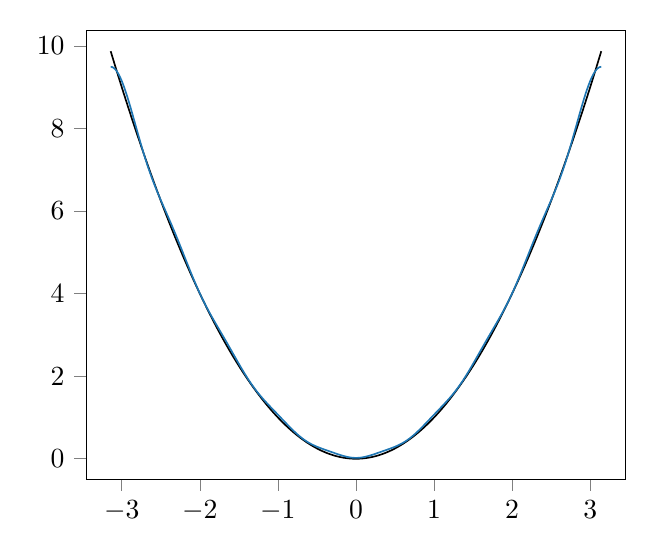
\begin{tikzpicture}

\definecolor{color0}{rgb}{0.12156862745098,0.466666666666667,0.705882352941177}

\begin{axis}[
xmin=-3.45575191894877, xmax=3.45575191894877,
ymin=-0.493374440832253, ymax=10.363079584038,
tick align=outside,
tick pos=left,
x grid style={white!69.01960784313725!black},
y grid style={white!69.01960784313725!black}
]
\addplot [semithick, black, forget plot]
table {%
-3.14159265358979 9.86960440108936
-3.12151857912596 9.74387823982856
-3.10144450466213 9.61895801549891
-3.0813704301983 9.49484372810043
-3.06129635573446 9.3715353776331
-3.04122228127063 9.24903296409694
-3.0211482068068 9.12733648749193
-3.00107413234297 9.00644594781808
-2.98100005787913 8.88636134507539
-2.9609259834153 8.76708267926386
-2.94085190895147 8.64860995038349
-2.92077783448764 8.53094315843428
-2.9007037600238 8.41408230341623
-2.88062968555997 8.29802738532933
-2.86055561109614 8.1827784041736
-2.8404815366323 8.06833535994902
-2.82040746216847 7.9546982526556
-2.80033338770464 7.84186708229335
-2.78025931324081 7.72984184886225
-2.76018523877697 7.61862255236231
-2.74011116431314 7.50820919279353
-2.72003708984931 7.3986017701559
-2.69996301538548 7.28980028444944
-2.67988894092164 7.18180473567413
-2.65981486645781 7.07461512382999
-2.63974079199398 6.968231448917
-2.61966671753015 6.86265371093517
-2.59959264306631 6.75788190988451
-2.57951856860248 6.653916045765
-2.55944449413865 6.55075611857665
-2.53937041967482 6.44840212831945
-2.51929634521098 6.34685407499342
-2.49922227074715 6.24611195859855
-2.47914819628332 6.14617577913484
-2.45907412181949 6.04704553660228
-2.43900004735565 5.94872123100088
-2.41892597289182 5.85120286233065
-2.39885189842799 5.75449043059157
-2.37877782396416 5.65858393578365
-2.35870374950032 5.56348337790689
-2.33862967503649 5.46918875696129
-2.31855560057266 5.37570007294684
-2.29848152610883 5.28301732586356
-2.27840745164499 5.19114051571144
-2.25833337718116 5.10006964249047
-2.23825930271733 5.00980470620066
-2.2181852282535 4.92034570684202
-2.19811115378966 4.83169264441453
-2.17803707932583 4.7438455189182
-2.157963004862 4.65680433035303
-2.13788893039817 4.57056907871901
-2.11781485593433 4.48513976401616
-2.0977407814705 4.40051638624447
-2.07766670700667 4.31669894540393
-2.05759263254284 4.23368744149456
-2.037518558079 4.15148187451634
-2.01744448361517 4.07008224446928
-1.99737040915134 3.98948855135338
-1.97729633468751 3.90970079516864
-1.95722226022367 3.83071897591506
-1.93714818575984 3.75254309359264
-1.91707411129601 3.67517314820138
-1.89700003683218 3.59860913974128
-1.87692596236834 3.52285106821233
-1.85685188790451 3.44789893361454
-1.83677781344068 3.37375273594792
-1.81670373897685 3.30041247521245
-1.79662966451301 3.22787815140814
-1.77655559004918 3.15614976453499
-1.75648151558535 3.085227314593
-1.73640744112152 3.01511080158217
-1.71633336665768 2.9458002255025
-1.69625929219385 2.87729558635398
-1.67618521773002 2.80959688413663
-1.65611114326619 2.74270411885043
-1.63603706880235 2.67661729049539
-1.61596299433852 2.61133639907152
-1.59588891987469 2.5468614445788
-1.57581484541085 2.48319242701724
-1.55574077094702 2.42032934638684
-1.53566669648319 2.35827220268759
-1.51559262201936 2.29702099591951
-1.49551854755552 2.23657572608259
-1.47544447309169 2.17693639317682
-1.45537039862786 2.11810299720221
-1.43529632416403 2.06007553815877
-1.41522224970019 2.00285401604648
-1.39514817523636 1.94643843086535
-1.37507410077253 1.89082878261538
-1.3550000263087 1.83602507129657
-1.33492595184486 1.78202729690892
-1.31485187738103 1.72883545945242
-1.2947778029172 1.67644955892709
-1.27470372845337 1.62486959533291
-1.25462965398953 1.5740955686699
-1.2345555795257 1.52412747893804
-1.21448150506187 1.47496532613734
-1.19440743059804 1.4266091102678
-1.1743333561342 1.37905883132942
-1.15425928167037 1.3323144893222
-1.13418520720654 1.28637608424614
-1.11411113274271 1.24124361610124
-1.09403705827887 1.19691708488749
-1.07396298381504 1.15339649060491
-1.05388890935121 1.11068183325348
-1.03381483488738 1.06877311283321
-1.01374076042354 1.0276703293441
-0.993666685959711 0.987373482786155
-0.973592611495878 0.947882573159364
-0.953518537032046 0.909197600463733
-0.933444462568213 0.87131856469926
-0.913370388104381 0.834245465865948
-0.893296313640549 0.797978303963793
-0.873222239176716 0.762517078992798
-0.853148164712883 0.727861790952961
-0.833074090249051 0.694012439844284
-0.813000015785218 0.660969025666765
-0.792925941321386 0.628731548420405
-0.772851866857553 0.597300008105205
-0.75277779239372 0.566674404721163
-0.732703717929888 0.536854738268281
-0.712629643466055 0.507841008746557
-0.692555569002223 0.479633216155992
-0.672481494538391 0.452231360496587
-0.652407420074558 0.425635441768341
-0.632333345610725 0.399845459971253
-0.612259271146893 0.374861415105324
-0.59218519668306 0.350683307170555
-0.572111122219228 0.327311136166944
-0.552037047755395 0.304744902094492
-0.531962973291563 0.2829846049532
-0.51188889882773 0.262030244743066
-0.491814824363897 0.241881821464091
-0.471740749900065 0.222539335116275
-0.451666675436233 0.204002785699619
-0.4315926009724 0.186272173214121
-0.411518526508567 0.169347497659783
-0.391444452044735 0.153228759036603
-0.371370377580902 0.137915957344582
-0.35129630311707 0.12340909258372
-0.331222228653237 0.109708164754017
-0.311148154189405 0.0968131738554735
-0.291074079725572 0.0847241198880886
-0.271000005261739 0.0734410028518628
-0.250925930797907 0.0629638227467959
-0.230851856334074 0.053292579572888
-0.210777781870242 0.0444272733301394
-0.19070370740641 0.0363679040185495
-0.170629632942577 0.0291144716381185
-0.150555558478744 0.0226669761888466
-0.130481484014912 0.0170254176707337
-0.110407409551079 0.0121897960837797
-0.0903333350872466 0.00816011142798478
-0.070259260623414 0.00493636370334882
-0.0501851861595815 0.00251855290987185
-0.0301111116957489 0.000906679047553864
-0.0100370372319163 0.000100742116394874
0.0100370372319163 0.000100742116394874
0.0301111116957484 0.000906679047553838
0.050185186159581 0.0025185529098718
0.0702592606234136 0.00493636370334876
0.0903333350872462 0.0081601114279847
0.110407409551079 0.0121897960837796
0.130481484014911 0.0170254176707336
0.150555558478744 0.0226669761888465
0.170629632942576 0.0291144716381184
0.190703707406409 0.0363679040185493
0.210777781870242 0.0444272733301392
0.230851856334074 0.053292579572888
0.250925930797906 0.0629638227467957
0.271000005261739 0.0734410028518625
0.291074079725572 0.0847241198880884
0.311148154189404 0.0968131738554732
0.331222228653237 0.109708164754017
0.351296303117069 0.12340909258372
0.371370377580902 0.137915957344582
0.391444452044734 0.153228759036602
0.411518526508567 0.169347497659782
0.4315926009724 0.186272173214121
0.451666675436232 0.204002785699619
0.471740749900065 0.222539335116275
0.491814824363897 0.241881821464091
0.511888898827729 0.262030244743065
0.531962973291562 0.282984604953199
0.552037047755395 0.304744902094492
0.572111122219227 0.327311136166944
0.59218519668306 0.350683307170554
0.612259271146892 0.374861415105324
0.632333345610725 0.399845459971253
0.652407420074558 0.42563544176834
0.67248149453839 0.452231360496587
0.692555569002223 0.479633216155992
0.712629643466055 0.507841008746557
0.732703717929887 0.53685473826828
0.75277779239372 0.566674404721163
0.772851866857553 0.597300008105204
0.792925941321385 0.628731548420405
0.813000015785218 0.660969025666764
0.83307409024905 0.694012439844283
0.853148164712883 0.72786179095296
0.873222239176715 0.762517078992796
0.893296313640548 0.797978303963792
0.91337038810438 0.834245465865946
0.933444462568213 0.87131856469926
0.953518537032045 0.909197600463732
0.973592611495878 0.947882573159364
0.993666685959711 0.987373482786154
1.01374076042354 1.0276703293441
1.03381483488738 1.06877311283321
1.05388890935121 1.11068183325348
1.07396298381504 1.15339649060491
1.09403705827887 1.19691708488749
1.11411113274271 1.24124361610124
1.13418520720654 1.28637608424614
1.15425928167037 1.3323144893222
1.1743333561342 1.37905883132942
1.19440743059804 1.4266091102678
1.21448150506187 1.47496532613734
1.2345555795257 1.52412747893804
1.25462965398953 1.5740955686699
1.27470372845337 1.62486959533291
1.2947778029172 1.67644955892709
1.31485187738103 1.72883545945242
1.33492595184486 1.78202729690891
1.3550000263087 1.83602507129657
1.37507410077253 1.89082878261538
1.39514817523636 1.94643843086535
1.41522224970019 2.00285401604648
1.43529632416403 2.06007553815877
1.45537039862786 2.11810299720221
1.47544447309169 2.17693639317682
1.49551854755552 2.23657572608258
1.51559262201936 2.29702099591951
1.53566669648319 2.35827220268759
1.55574077094702 2.42032934638683
1.57581484541085 2.48319242701724
1.59588891987469 2.5468614445788
1.61596299433852 2.61133639907151
1.63603706880235 2.67661729049539
1.65611114326618 2.74270411885043
1.67618521773002 2.80959688413663
1.69625929219385 2.87729558635398
1.71633336665768 2.9458002255025
1.73640744112152 3.01511080158217
1.75648151558535 3.085227314593
1.77655559004918 3.15614976453499
1.79662966451301 3.22787815140814
1.81670373897684 3.30041247521245
1.83677781344068 3.37375273594792
1.85685188790451 3.44789893361454
1.87692596236834 3.52285106821233
1.89700003683217 3.59860913974127
1.91707411129601 3.67517314820138
1.93714818575984 3.75254309359264
1.95722226022367 3.83071897591506
1.97729633468751 3.90970079516864
1.99737040915134 3.98948855135338
2.01744448361517 4.07008224446928
2.037518558079 4.15148187451634
2.05759263254284 4.23368744149456
2.07766670700667 4.31669894540393
2.0977407814705 4.40051638624447
2.11781485593433 4.48513976401616
2.13788893039817 4.57056907871901
2.157963004862 4.65680433035303
2.17803707932583 4.7438455189182
2.19811115378966 4.83169264441453
2.2181852282535 4.92034570684202
2.23825930271733 5.00980470620066
2.25833337718116 5.10006964249047
2.27840745164499 5.19114051571143
2.29848152610883 5.28301732586356
2.31855560057266 5.37570007294684
2.33862967503649 5.46918875696128
2.35870374950032 5.56348337790688
2.37877782396416 5.65858393578364
2.39885189842799 5.75449043059156
2.41892597289182 5.85120286233064
2.43900004735565 5.94872123100088
2.45907412181949 6.04704553660228
2.47914819628332 6.14617577913483
2.49922227074715 6.24611195859855
2.51929634521098 6.34685407499342
2.53937041967482 6.44840212831945
2.55944449413865 6.55075611857665
2.57951856860248 6.653916045765
2.59959264306631 6.75788190988451
2.61966671753015 6.86265371093517
2.63974079199398 6.968231448917
2.65981486645781 7.07461512382999
2.67988894092164 7.18180473567413
2.69996301538548 7.28980028444943
2.72003708984931 7.3986017701559
2.74011116431314 7.50820919279352
2.76018523877697 7.6186225523623
2.78025931324081 7.72984184886224
2.80033338770464 7.84186708229334
2.82040746216847 7.9546982526556
2.8404815366323 8.06833535994902
2.86055561109614 8.18277840417359
2.88062968555997 8.29802738532933
2.9007037600238 8.41408230341622
2.92077783448763 8.53094315843428
2.94085190895147 8.64860995038349
2.9609259834153 8.76708267926386
2.98100005787913 8.88636134507539
3.00107413234297 9.00644594781808
3.0211482068068 9.12733648749193
3.04122228127063 9.24903296409694
3.06129635573446 9.3715353776331
3.0813704301983 9.49484372810043
3.10144450466213 9.61895801549891
3.12151857912596 9.74387823982856
3.14159265358979 9.86960440108936
};
\addplot [semithick, color0, forget plot]
table {%
-3.14159265358979 9.4924042579995
-3.12151857912596 9.48515853326787
-3.10144450466213 9.46351358391951
-3.0813704301983 9.4277440907077
-3.06129635573446 9.37830126005392
-3.04122228127063 9.31580310929641
-3.0211482068068 9.24102121595968
-3.00107413234297 9.15486426926964
-2.98100005787913 9.0583588424478
-2.9609259834153 8.95262787303981
-2.94085190895147 8.83886739379956
-2.92077783448764 8.71832209698257
-2.9007037600238 8.59226033925514
-2.88062968555997 8.46194920221535
-2.86055561109614 8.32863021463946
-2.8404815366323 8.19349631738403
-2.82040746216847 8.05767061122334
-2.80033338770464 7.92218737305762
-2.78025931324081 7.78797575855838
-2.76018523877697 7.65584653144227
-2.74011116431314 7.52648207348484
-2.72003708984931 7.40042983761983
-2.69996301538548 7.27809931167577
-2.67988894092164 7.15976246519976
-2.65981486645781 7.04555755910739
-2.63974079199398 6.93549611017992
-2.61966671753015 6.82947272213012
-2.59959264306631 6.72727742425949
-2.57951856860248 6.62861009950536
-2.55944449413865 6.53309653744387
-2.53937041967482 6.44030561568797
-2.51929634521098 6.34976709578619
-2.49922227074715 6.26098951742871
-2.47914819628332 6.17347768729896
-2.45907412181949 6.08674928563113
-2.43900004735565 6.00035015339711
-2.41892597289182 5.9138678746274
-2.39885189842799 5.82694332991877
-2.37877782396416 5.73927996667959
-2.35870374950032 5.65065060688815
-2.33862967503649 5.5609016917324
-2.31855560057266 5.46995494204401
-2.29848152610883 5.37780649152916
-2.27840745164499 5.28452362411537
-2.25833337718116 5.19023931511453
-2.23825930271733 5.09514483640351
-2.2181852282535 4.9994807367782
-2.19811115378966 4.90352654869956
-2.17803707932583 4.80758960083512
-2.157963004862 4.71199333150562
-2.13788893039817 4.61706550116779
-2.11781485593433 4.5231266925929
-2.0977407814705 4.43047946601204
-2.07766670700667 4.33939850412832
-2.05759263254284 4.25012203980502
-2.037518558079 4.16284480896737
-2.01744448361517 4.07771271457401
-1.99737040915134 3.99481932635664
-1.97729633468751 3.91420427743703
-1.95722226022367 3.83585355498501
-1.93714818575984 3.75970161983292
-1.91707411129601 3.68563523136746
-1.89700003683218 3.61349880088317
-1.87692596236834 3.54310105049924
-1.85685188790451 3.4742227170514
-1.83677781344068 3.40662501211801
-1.81670373897685 3.34005853124537
-1.79662966451301 3.27427229788045
-1.77655559004918 3.209022630531
-1.75648151558535 3.14408153494167
-1.73640744112152 3.07924434595795
-1.71633336665768 3.01433637530728
-1.69625929219385 2.94921836054677
-1.67618521773002 2.88379055547926
-1.65611114326619 2.81799535181642
-1.63603706880235 2.75181837404736
-1.61596299433852 2.68528804256918
-1.59588891987469 2.61847365236859
-1.57581484541085 2.55148206418545
-1.55574077094702 2.48445315052798
-1.53566669648319 2.4175541786982
-1.51559262201936 2.35097334588989
-1.49551854755552 2.28491270645147
-1.47544447309169 2.21958074785336
-1.45537039862786 2.15518487934996
-1.43529632416403 2.09192409567464
-1.41522224970019 2.0299820675517
-1.39514817523636 1.96952089184698
-1.37507410077253 1.91067570757892
-1.3550000263087 1.85355035078938
-1.33492595184486 1.79821418265257
-1.31485187738103 1.74470018256957
-1.2947778029172 1.6930043528602
-1.27470372845337 1.64308643559293
-1.25462965398953 1.59487189666762
-1.2345555795257 1.54825508902346
-1.21448150506187 1.50310346723081
-1.19440743059804 1.4592626910442
-1.1743333561342 1.41656242686669
-1.15425928167037 1.37482263440374
-1.13418520720654 1.33386011172414
-1.11411113274271 1.29349506588505
-1.09403705827887 1.25355747832958
-1.07396298381504 1.21389304426454
-1.05388890935121 1.17436848273821
-1.03381483488738 1.13487603847815
-1.01374076042354 1.09533702680565
-0.993666685959711 1.05570430801245
-0.973592611495878 1.01596361621026
-0.953518537032046 0.976133708476876
-0.933444462568213 0.936265341697924
-0.913370388104381 0.896439125398758
-0.893296313640549 0.856762337673891
-0.873222239176716 0.81736482673172
-0.853148164712883 0.778394151389156
-0.833074090249051 0.740010139051205
-0.813000015785218 0.702379058472965
-0.792925941321386 0.665667616332605
-0.772851866857553 0.630036990996683
-0.75277779239372 0.595637113743441
-0.732703717929888 0.562601397292609
-0.712629643466055 0.531042094189503
-0.692555569002223 0.50104644405801
-0.672481494538391 0.472673739833373
-0.652407420074558 0.445953409852044
-0.632333345610725 0.420884176295629
-0.612259271146893 0.397434312242833
-0.59218519668306 0.375542980817573
-0.572111122219228 0.355122601982728
-0.552037047755395 0.336062156730654
-0.531962973291563 0.318231305995047
-0.51188889882773 0.301485173662232
-0.491814824363897 0.285669620540488
-0.471740749900065 0.270626819808209
-0.451666675436233 0.256200934841982
-0.4315926009724 0.242243697725916
-0.411518526508567 0.228619691220398
-0.391444452044735 0.215211148333839
-0.371370377580902 0.201922101468543
-0.35129630311707 0.188681736753147
-0.331222228653237 0.175446837781721
-0.311148154189405 0.162203235537263
-0.291074079725572 0.148966216634969
-0.271000005261739 0.135779878935453
-0.250925930797907 0.122715460756837
-0.230851856334074 0.109868706059197
-0.210777781870242 0.0973563618263262
-0.19070370740641 0.0853119342528021
-0.170629632942577 0.0738808562063125
-0.150555558478744 0.0632152388836666
-0.130481484014912 0.0534683949108548
-0.110407409551079 0.044789327864259
-0.0903333350872466 0.0373173840532166
-0.070259260623414 0.0311772563841832
-0.0501851861595815 0.0264745174437659
-0.0301111116957489 0.0232918400432314
-0.0100370372319163 0.0216860390276237
0.0100370372319163 0.0216860390276237
0.0301111116957484 0.0232918400432309
0.050185186159581 0.0264745174437655
0.0702592606234136 0.0311772563841823
0.0903333350872462 0.0373173840532171
0.110407409551079 0.044789327864259
0.130481484014911 0.0534683949108534
0.150555558478744 0.0632152388836666
0.170629632942576 0.0738808562063125
0.190703707406409 0.0853119342528013
0.210777781870242 0.0973563618263258
0.230851856334074 0.109868706059197
0.250925930797906 0.122715460756836
0.271000005261739 0.135779878935452
0.291074079725572 0.148966216634969
0.311148154189404 0.162203235537262
0.331222228653237 0.175446837781722
0.351296303117069 0.188681736753147
0.371370377580902 0.201922101468543
0.391444452044734 0.215211148333837
0.411518526508567 0.228619691220399
0.4315926009724 0.242243697725917
0.451666675436232 0.256200934841981
0.471740749900065 0.270626819808209
0.491814824363897 0.285669620540489
0.511888898827729 0.301485173662231
0.531962973291562 0.318231305995047
0.552037047755395 0.336062156730653
0.572111122219227 0.355122601982728
0.59218519668306 0.375542980817572
0.612259271146892 0.397434312242833
0.632333345610725 0.420884176295628
0.652407420074558 0.445953409852043
0.67248149453839 0.472673739833371
0.692555569002223 0.50104644405801
0.712629643466055 0.531042094189503
0.732703717929887 0.562601397292608
0.75277779239372 0.59563711374344
0.772851866857553 0.630036990996682
0.792925941321385 0.665667616332604
0.813000015785218 0.702379058472964
0.83307409024905 0.740010139051204
0.853148164712883 0.778394151389156
0.873222239176715 0.817364826731718
0.893296313640548 0.856762337673889
0.91337038810438 0.896439125398756
0.933444462568213 0.936265341697923
0.953518537032045 0.976133708476876
0.973592611495878 1.01596361621026
0.993666685959711 1.05570430801245
1.01374076042354 1.09533702680565
1.03381483488738 1.13487603847815
1.05388890935121 1.17436848273821
1.07396298381504 1.21389304426454
1.09403705827887 1.25355747832958
1.11411113274271 1.29349506588505
1.13418520720654 1.33386011172414
1.15425928167037 1.37482263440374
1.1743333561342 1.41656242686669
1.19440743059804 1.4592626910442
1.21448150506187 1.50310346723081
1.2345555795257 1.54825508902346
1.25462965398953 1.59487189666762
1.27470372845337 1.64308643559293
1.2947778029172 1.6930043528602
1.31485187738103 1.74470018256957
1.33492595184486 1.79821418265257
1.3550000263087 1.85355035078938
1.37507410077253 1.91067570757892
1.39514817523636 1.96952089184698
1.41522224970019 2.0299820675517
1.43529632416403 2.09192409567464
1.45537039862786 2.15518487934996
1.47544447309169 2.21958074785336
1.49551854755552 2.28491270645147
1.51559262201936 2.35097334588989
1.53566669648319 2.4175541786982
1.55574077094702 2.48445315052798
1.57581484541085 2.55148206418545
1.59588891987469 2.61847365236859
1.61596299433852 2.68528804256918
1.63603706880235 2.75181837404736
1.65611114326618 2.81799535181642
1.67618521773002 2.88379055547926
1.69625929219385 2.94921836054677
1.71633336665768 3.01433637530728
1.73640744112152 3.07924434595795
1.75648151558535 3.14408153494167
1.77655559004918 3.209022630531
1.79662966451301 3.27427229788045
1.81670373897684 3.34005853124537
1.83677781344068 3.40662501211801
1.85685188790451 3.4742227170514
1.87692596236834 3.54310105049924
1.89700003683217 3.61349880088316
1.91707411129601 3.68563523136745
1.93714818575984 3.75970161983291
1.95722226022367 3.835853554985
1.97729633468751 3.91420427743703
1.99737040915134 3.99481932635664
2.01744448361517 4.07771271457401
2.037518558079 4.16284480896737
2.05759263254284 4.25012203980502
2.07766670700667 4.33939850412832
2.0977407814705 4.43047946601204
2.11781485593433 4.5231266925929
2.13788893039817 4.61706550116779
2.157963004862 4.71199333150562
2.17803707932583 4.80758960083512
2.19811115378966 4.90352654869956
2.2181852282535 4.9994807367782
2.23825930271733 5.09514483640351
2.25833337718116 5.19023931511453
2.27840745164499 5.28452362411536
2.29848152610883 5.37780649152915
2.31855560057266 5.46995494204401
2.33862967503649 5.5609016917324
2.35870374950032 5.65065060688815
2.37877782396416 5.73927996667959
2.39885189842799 5.82694332991877
2.41892597289182 5.9138678746274
2.43900004735565 6.00035015339711
2.45907412181949 6.08674928563113
2.47914819628332 6.17347768729896
2.49922227074715 6.2609895174287
2.51929634521098 6.34976709578619
2.53937041967482 6.44030561568797
2.55944449413865 6.53309653744387
2.57951856860248 6.62861009950536
2.59959264306631 6.72727742425949
2.61966671753015 6.82947272213012
2.63974079199398 6.93549611017992
2.65981486645781 7.04555755910739
2.67988894092164 7.15976246519976
2.69996301538548 7.27809931167576
2.72003708984931 7.40042983761982
2.74011116431314 7.52648207348484
2.76018523877697 7.65584653144227
2.78025931324081 7.78797575855837
2.80033338770464 7.92218737305762
2.82040746216847 8.05767061122334
2.8404815366323 8.19349631738403
2.86055561109614 8.32863021463946
2.88062968555997 8.46194920221534
2.9007037600238 8.59226033925514
2.92077783448763 8.71832209698257
2.94085190895147 8.83886739379956
2.9609259834153 8.9526278730398
2.98100005787913 9.0583588424478
3.00107413234297 9.15486426926964
3.0211482068068 9.24102121595968
3.04122228127063 9.31580310929641
3.06129635573446 9.37830126005392
3.0813704301983 9.4277440907077
3.10144450466213 9.46351358391951
3.12151857912596 9.48515853326787
3.14159265358979 9.4924042579995
};
\path [opacity=0] (axis cs:1,13)
--(axis cs:1,13);

\path [opacity=0] (axis cs:13,1)
--(axis cs:13,1);

\end{axis}

\end{tikzpicture}
\caption{\label{fig:fourier_approx}Fourier Series approximation of $x^2$.}
\end{figure}

\subsection{Wavelet Analysis}%
\label{sub:wavelet_analysis}

Now we will use Wavelet analysis to approximate the function of $x^2$. For this approximation we will be using the Haar Wavelet basis that we have focused on for this paper. Once again the first step is to find the wavelet coefficients.

\begin{align}
	a_k&=\frac{\left<x^2,2^\frac{j}{2}\Psi\left(2^jx-k\right)\right>}{{\Vert 2^\frac{j}{2}\Psi\left(2^jx-k\right)\Vert}^2}
\end{align}

Since the basis is normal as we proved earlier, we just need to solve the inner product

\begin{align}
	\left<x^2,2^\frac{j}{2}\Psi\left(2^jx-k\right)\right> &= \int_{-L}^{L}x^2\cdot 2^\frac{j}{2}\Psi\left(2^jx-k\right)dx\\
	&=2^\frac{j}{2}\left[\int_{\frac{k}{2^j}}^{\frac{1}{2^j}\left(\frac{1}{2}+k\right)}x^2dx+\int_{\frac{1}{2^j}\left(\frac{1}{2}+k\right)}^{\frac{1}{2^j}\left(1+k\right)}-x^2dx\right]\\
	&= 2^\frac{j}{2}\left[\frac{k^3}{3\cdot 2^{3j}}-\frac{\left(\frac{1}{2}+k\right)^3}{3\cdot 2^{3j}}-\frac{\left(\frac{1}{2}+k\right)^3}{3\cdot 2^{3j}}+\frac{\left(1+k\right)^3}{3\cdot 2^{3j}}\right]\\
	&=\frac{1}{3}2^{-\frac{5j}{2}}\left(\frac{3k}{2}+\frac{3}{4}\right)
\end{align}
\todo{Not quite right, needs a fudge factor determined by j's lowest index, and should be negative. I will redo the math.}
We can now use this function to create the Haar series representation of $x^2$ which is written like so

\begin{align}
	u(x)=\sum_{k=-\infty}^{\infty}\sum_{j=-\infty}^{\infty}\frac{1}{3}2^{-\frac{5j}{2}}\left(\frac{3k}{2}+\frac{3}{4}\right)2^\frac{j}{2}\Psi\left(2^jx-k\right)
\end{align}

Once again the resulting graph of the approximation is shown in Figure~\ref{fig:haar_approx}. We can see that it is not as accurate as the Fourier series approximation, but looking beyond the bounds, the Haar series continues to approximate the function, while the Fourier series begins periodic motion.

\begin{figure}
\centering
% This file was created by matplotlib2tikz v0.6.16.
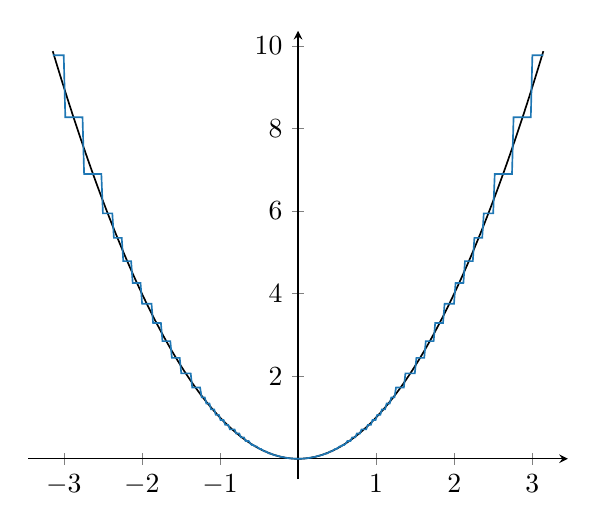
\begin{tikzpicture}

\definecolor{color0}{rgb}{0.12156862745098,0.466666666666667,0.705882352941177}

\begin{axis}[
axis x line=center,
axis y line=center,
xmin=-3.45575191894877, xmax=3.45575191894877,
ymin=-0.493374440832253, ymax=10.363079584038,
x grid style={white!69.01960784313725!black},
y grid style={white!69.01960784313725!black}
]
\addplot [semithick, black, forget plot]
table {%
-3.14159265358979 9.86960440108936
-3.12151857912596 9.74387823982856
-3.10144450466213 9.61895801549891
-3.0813704301983 9.49484372810043
-3.06129635573446 9.3715353776331
-3.04122228127063 9.24903296409694
-3.0211482068068 9.12733648749193
-3.00107413234297 9.00644594781808
-2.98100005787913 8.88636134507539
-2.9609259834153 8.76708267926386
-2.94085190895147 8.64860995038349
-2.92077783448764 8.53094315843428
-2.9007037600238 8.41408230341623
-2.88062968555997 8.29802738532933
-2.86055561109614 8.1827784041736
-2.8404815366323 8.06833535994902
-2.82040746216847 7.9546982526556
-2.80033338770464 7.84186708229335
-2.78025931324081 7.72984184886225
-2.76018523877697 7.61862255236231
-2.74011116431314 7.50820919279353
-2.72003708984931 7.3986017701559
-2.69996301538548 7.28980028444944
-2.67988894092164 7.18180473567413
-2.65981486645781 7.07461512382999
-2.63974079199398 6.968231448917
-2.61966671753015 6.86265371093517
-2.59959264306631 6.75788190988451
-2.57951856860248 6.653916045765
-2.55944449413865 6.55075611857665
-2.53937041967482 6.44840212831945
-2.51929634521098 6.34685407499342
-2.49922227074715 6.24611195859855
-2.47914819628332 6.14617577913484
-2.45907412181949 6.04704553660228
-2.43900004735565 5.94872123100088
-2.41892597289182 5.85120286233065
-2.39885189842799 5.75449043059157
-2.37877782396416 5.65858393578365
-2.35870374950032 5.56348337790689
-2.33862967503649 5.46918875696129
-2.31855560057266 5.37570007294684
-2.29848152610883 5.28301732586356
-2.27840745164499 5.19114051571144
-2.25833337718116 5.10006964249047
-2.23825930271733 5.00980470620066
-2.2181852282535 4.92034570684202
-2.19811115378966 4.83169264441453
-2.17803707932583 4.7438455189182
-2.157963004862 4.65680433035303
-2.13788893039817 4.57056907871901
-2.11781485593433 4.48513976401616
-2.0977407814705 4.40051638624447
-2.07766670700667 4.31669894540393
-2.05759263254284 4.23368744149456
-2.037518558079 4.15148187451634
-2.01744448361517 4.07008224446928
-1.99737040915134 3.98948855135338
-1.97729633468751 3.90970079516864
-1.95722226022367 3.83071897591506
-1.93714818575984 3.75254309359264
-1.91707411129601 3.67517314820138
-1.89700003683218 3.59860913974128
-1.87692596236834 3.52285106821233
-1.85685188790451 3.44789893361454
-1.83677781344068 3.37375273594792
-1.81670373897685 3.30041247521245
-1.79662966451301 3.22787815140814
-1.77655559004918 3.15614976453499
-1.75648151558535 3.085227314593
-1.73640744112152 3.01511080158217
-1.71633336665768 2.9458002255025
-1.69625929219385 2.87729558635398
-1.67618521773002 2.80959688413663
-1.65611114326619 2.74270411885043
-1.63603706880235 2.67661729049539
-1.61596299433852 2.61133639907152
-1.59588891987469 2.5468614445788
-1.57581484541085 2.48319242701724
-1.55574077094702 2.42032934638684
-1.53566669648319 2.35827220268759
-1.51559262201936 2.29702099591951
-1.49551854755552 2.23657572608259
-1.47544447309169 2.17693639317682
-1.45537039862786 2.11810299720221
-1.43529632416403 2.06007553815877
-1.41522224970019 2.00285401604648
-1.39514817523636 1.94643843086535
-1.37507410077253 1.89082878261538
-1.3550000263087 1.83602507129657
-1.33492595184486 1.78202729690892
-1.31485187738103 1.72883545945242
-1.2947778029172 1.67644955892709
-1.27470372845337 1.62486959533291
-1.25462965398953 1.5740955686699
-1.2345555795257 1.52412747893804
-1.21448150506187 1.47496532613734
-1.19440743059804 1.4266091102678
-1.1743333561342 1.37905883132942
-1.15425928167037 1.3323144893222
-1.13418520720654 1.28637608424614
-1.11411113274271 1.24124361610124
-1.09403705827887 1.19691708488749
-1.07396298381504 1.15339649060491
-1.05388890935121 1.11068183325348
-1.03381483488738 1.06877311283321
-1.01374076042354 1.0276703293441
-0.993666685959711 0.987373482786155
-0.973592611495878 0.947882573159364
-0.953518537032046 0.909197600463733
-0.933444462568213 0.87131856469926
-0.913370388104381 0.834245465865948
-0.893296313640549 0.797978303963793
-0.873222239176716 0.762517078992798
-0.853148164712883 0.727861790952961
-0.833074090249051 0.694012439844284
-0.813000015785218 0.660969025666765
-0.792925941321386 0.628731548420405
-0.772851866857553 0.597300008105205
-0.75277779239372 0.566674404721163
-0.732703717929888 0.536854738268281
-0.712629643466055 0.507841008746557
-0.692555569002223 0.479633216155992
-0.672481494538391 0.452231360496587
-0.652407420074558 0.425635441768341
-0.632333345610725 0.399845459971253
-0.612259271146893 0.374861415105324
-0.59218519668306 0.350683307170555
-0.572111122219228 0.327311136166944
-0.552037047755395 0.304744902094492
-0.531962973291563 0.2829846049532
-0.51188889882773 0.262030244743066
-0.491814824363897 0.241881821464091
-0.471740749900065 0.222539335116275
-0.451666675436233 0.204002785699619
-0.4315926009724 0.186272173214121
-0.411518526508567 0.169347497659783
-0.391444452044735 0.153228759036603
-0.371370377580902 0.137915957344582
-0.35129630311707 0.12340909258372
-0.331222228653237 0.109708164754017
-0.311148154189405 0.0968131738554735
-0.291074079725572 0.0847241198880886
-0.271000005261739 0.0734410028518628
-0.250925930797907 0.0629638227467959
-0.230851856334074 0.053292579572888
-0.210777781870242 0.0444272733301394
-0.19070370740641 0.0363679040185495
-0.170629632942577 0.0291144716381185
-0.150555558478744 0.0226669761888466
-0.130481484014912 0.0170254176707337
-0.110407409551079 0.0121897960837797
-0.0903333350872466 0.00816011142798478
-0.070259260623414 0.00493636370334882
-0.0501851861595815 0.00251855290987185
-0.0301111116957489 0.000906679047553864
-0.0100370372319163 0.000100742116394874
0.0100370372319163 0.000100742116394874
0.0301111116957484 0.000906679047553838
0.050185186159581 0.0025185529098718
0.0702592606234136 0.00493636370334876
0.0903333350872462 0.0081601114279847
0.110407409551079 0.0121897960837796
0.130481484014911 0.0170254176707336
0.150555558478744 0.0226669761888465
0.170629632942576 0.0291144716381184
0.190703707406409 0.0363679040185493
0.210777781870242 0.0444272733301392
0.230851856334074 0.053292579572888
0.250925930797906 0.0629638227467957
0.271000005261739 0.0734410028518625
0.291074079725572 0.0847241198880884
0.311148154189404 0.0968131738554732
0.331222228653237 0.109708164754017
0.351296303117069 0.12340909258372
0.371370377580902 0.137915957344582
0.391444452044734 0.153228759036602
0.411518526508567 0.169347497659782
0.4315926009724 0.186272173214121
0.451666675436232 0.204002785699619
0.471740749900065 0.222539335116275
0.491814824363897 0.241881821464091
0.511888898827729 0.262030244743065
0.531962973291562 0.282984604953199
0.552037047755395 0.304744902094492
0.572111122219227 0.327311136166944
0.59218519668306 0.350683307170554
0.612259271146892 0.374861415105324
0.632333345610725 0.399845459971253
0.652407420074558 0.42563544176834
0.67248149453839 0.452231360496587
0.692555569002223 0.479633216155992
0.712629643466055 0.507841008746557
0.732703717929887 0.53685473826828
0.75277779239372 0.566674404721163
0.772851866857553 0.597300008105204
0.792925941321385 0.628731548420405
0.813000015785218 0.660969025666764
0.83307409024905 0.694012439844283
0.853148164712883 0.72786179095296
0.873222239176715 0.762517078992796
0.893296313640548 0.797978303963792
0.91337038810438 0.834245465865946
0.933444462568213 0.87131856469926
0.953518537032045 0.909197600463732
0.973592611495878 0.947882573159364
0.993666685959711 0.987373482786154
1.01374076042354 1.0276703293441
1.03381483488738 1.06877311283321
1.05388890935121 1.11068183325348
1.07396298381504 1.15339649060491
1.09403705827887 1.19691708488749
1.11411113274271 1.24124361610124
1.13418520720654 1.28637608424614
1.15425928167037 1.3323144893222
1.1743333561342 1.37905883132942
1.19440743059804 1.4266091102678
1.21448150506187 1.47496532613734
1.2345555795257 1.52412747893804
1.25462965398953 1.5740955686699
1.27470372845337 1.62486959533291
1.2947778029172 1.67644955892709
1.31485187738103 1.72883545945242
1.33492595184486 1.78202729690891
1.3550000263087 1.83602507129657
1.37507410077253 1.89082878261538
1.39514817523636 1.94643843086535
1.41522224970019 2.00285401604648
1.43529632416403 2.06007553815877
1.45537039862786 2.11810299720221
1.47544447309169 2.17693639317682
1.49551854755552 2.23657572608258
1.51559262201936 2.29702099591951
1.53566669648319 2.35827220268759
1.55574077094702 2.42032934638683
1.57581484541085 2.48319242701724
1.59588891987469 2.5468614445788
1.61596299433852 2.61133639907151
1.63603706880235 2.67661729049539
1.65611114326618 2.74270411885043
1.67618521773002 2.80959688413663
1.69625929219385 2.87729558635398
1.71633336665768 2.9458002255025
1.73640744112152 3.01511080158217
1.75648151558535 3.085227314593
1.77655559004918 3.15614976453499
1.79662966451301 3.22787815140814
1.81670373897684 3.30041247521245
1.83677781344068 3.37375273594792
1.85685188790451 3.44789893361454
1.87692596236834 3.52285106821233
1.89700003683217 3.59860913974127
1.91707411129601 3.67517314820138
1.93714818575984 3.75254309359264
1.95722226022367 3.83071897591506
1.97729633468751 3.90970079516864
1.99737040915134 3.98948855135338
2.01744448361517 4.07008224446928
2.037518558079 4.15148187451634
2.05759263254284 4.23368744149456
2.07766670700667 4.31669894540393
2.0977407814705 4.40051638624447
2.11781485593433 4.48513976401616
2.13788893039817 4.57056907871901
2.157963004862 4.65680433035303
2.17803707932583 4.7438455189182
2.19811115378966 4.83169264441453
2.2181852282535 4.92034570684202
2.23825930271733 5.00980470620066
2.25833337718116 5.10006964249047
2.27840745164499 5.19114051571143
2.29848152610883 5.28301732586356
2.31855560057266 5.37570007294684
2.33862967503649 5.46918875696128
2.35870374950032 5.56348337790688
2.37877782396416 5.65858393578364
2.39885189842799 5.75449043059156
2.41892597289182 5.85120286233064
2.43900004735565 5.94872123100088
2.45907412181949 6.04704553660228
2.47914819628332 6.14617577913483
2.49922227074715 6.24611195859855
2.51929634521098 6.34685407499342
2.53937041967482 6.44840212831945
2.55944449413865 6.55075611857665
2.57951856860248 6.653916045765
2.59959264306631 6.75788190988451
2.61966671753015 6.86265371093517
2.63974079199398 6.968231448917
2.65981486645781 7.07461512382999
2.67988894092164 7.18180473567413
2.69996301538548 7.28980028444943
2.72003708984931 7.3986017701559
2.74011116431314 7.50820919279352
2.76018523877697 7.6186225523623
2.78025931324081 7.72984184886224
2.80033338770464 7.84186708229334
2.82040746216847 7.9546982526556
2.8404815366323 8.06833535994902
2.86055561109614 8.18277840417359
2.88062968555997 8.29802738532933
2.9007037600238 8.41408230341622
2.92077783448763 8.53094315843428
2.94085190895147 8.64860995038349
2.9609259834153 8.76708267926386
2.98100005787913 8.88636134507539
3.00107413234297 9.00644594781808
3.0211482068068 9.12733648749193
3.04122228127063 9.24903296409694
3.06129635573446 9.3715353776331
3.0813704301983 9.49484372810043
3.10144450466213 9.61895801549891
3.12151857912596 9.74387823982856
3.14159265358979 9.86960440108936
};
\addplot [semithick, color0, forget plot]
table {%
-3.14159265358979 9.77083330001915
-3.12151857912596 9.77083330001915
-3.10144450466213 9.77083330001915
-3.0813704301983 9.77083330001915
-3.06129635573446 9.77083330001915
-3.04122228127063 9.77083330001915
-3.0211482068068 9.77083330001915
-3.00107413234297 9.77083330001915
-2.98100005787913 8.27083330001915
-2.9609259834153 8.27083330001915
-2.94085190895147 8.27083330001915
-2.92077783448764 8.27083330001915
-2.9007037600238 8.27083330001915
-2.88062968555997 8.27083330001915
-2.86055561109614 8.27083330001915
-2.8404815366323 8.27083330001915
-2.82040746216847 8.27083330001915
-2.80033338770464 8.27083330001915
-2.78025931324081 8.27083330001915
-2.76018523877697 8.27083330001915
-2.74011116431314 6.89583330001915
-2.72003708984931 6.89583330001915
-2.69996301538548 6.89583330001915
-2.67988894092164 6.89583330001915
-2.65981486645781 6.89583330001915
-2.63974079199398 6.89583330001915
-2.61966671753015 6.89583330001915
-2.59959264306631 6.89583330001915
-2.57951856860248 6.89583330001915
-2.55944449413865 6.89583330001915
-2.53937041967482 6.89583330001915
-2.51929634521098 6.89583330001915
-2.49922227074715 5.94270830001915
-2.47914819628332 5.94270830001915
-2.45907412181949 5.94270830001915
-2.43900004735565 5.94270830001915
-2.41892597289182 5.94270830001915
-2.39885189842799 5.94270830001915
-2.37877782396416 5.94270830001915
-2.35870374950032 5.34895830001915
-2.33862967503649 5.34895830001915
-2.31855560057266 5.34895830001915
-2.29848152610883 5.34895830001915
-2.27840745164499 5.34895830001915
-2.25833337718116 5.34895830001915
-2.23825930271733 4.78645830001915
-2.2181852282535 4.78645830001915
-2.19811115378966 4.78645830001915
-2.17803707932583 4.78645830001915
-2.157963004862 4.78645830001915
-2.13788893039817 4.78645830001915
-2.11781485593433 4.25520830001915
-2.0977407814705 4.25520830001915
-2.07766670700667 4.25520830001915
-2.05759263254284 4.25520830001915
-2.037518558079 4.25520830001915
-2.01744448361517 4.25520830001915
-1.99737040915134 3.75520830001915
-1.97729633468751 3.75520830001915
-1.95722226022367 3.75520830001915
-1.93714818575984 3.75520830001915
-1.91707411129601 3.75520830001915
-1.89700003683218 3.75520830001915
-1.87692596236834 3.75520830001915
-1.85685188790451 3.28645830001915
-1.83677781344068 3.28645830001915
-1.81670373897685 3.28645830001915
-1.79662966451301 3.28645830001915
-1.77655559004918 3.28645830001915
-1.75648151558535 3.28645830001915
-1.73640744112152 2.84895830001915
-1.71633336665768 2.84895830001915
-1.69625929219385 2.84895830001915
-1.67618521773002 2.84895830001915
-1.65611114326619 2.84895830001915
-1.63603706880235 2.84895830001915
-1.61596299433852 2.44270830001915
-1.59588891987469 2.44270830001915
-1.57581484541085 2.44270830001915
-1.55574077094702 2.44270830001915
-1.53566669648319 2.44270830001915
-1.51559262201936 2.44270830001915
-1.49551854755552 2.06770830001915
-1.47544447309169 2.06770830001915
-1.45537039862786 2.06770830001915
-1.43529632416403 2.06770830001915
-1.41522224970019 2.06770830001915
-1.39514817523636 2.06770830001915
-1.37507410077253 2.06770830001915
-1.3550000263087 1.72395830001915
-1.33492595184486 1.72395830001915
-1.31485187738103 1.72395830001915
-1.2947778029172 1.72395830001915
-1.27470372845337 1.72395830001915
-1.25462965398953 1.72395830001915
-1.2345555795257 1.48567705001915
-1.21448150506187 1.48567705001915
-1.19440743059804 1.48567705001915
-1.1743333561342 1.33723955001915
-1.15425928167037 1.33723955001915
-1.13418520720654 1.33723955001915
-1.11411113274271 1.19661455001915
-1.09403705827887 1.19661455001915
-1.07396298381504 1.19661455001915
-1.05388890935121 1.06380205001915
-1.03381483488738 1.06380205001915
-1.01374076042354 1.06380205001915
-0.993666685959711 0.938802050019149
-0.973592611495878 0.938802050019149
-0.953518537032046 0.938802050019149
-0.933444462568213 0.821614550019149
-0.913370388104381 0.821614550019149
-0.893296313640549 0.821614550019149
-0.873222239176716 0.712239550019149
-0.853148164712883 0.712239550019149
-0.833074090249051 0.712239550019149
-0.813000015785218 0.712239550019149
-0.792925941321386 0.610677050019149
-0.772851866857553 0.610677050019149
-0.75277779239372 0.610677050019149
-0.732703717929888 0.516927050019149
-0.712629643466055 0.516927050019149
-0.692555569002223 0.516927050019149
-0.672481494538391 0.430989550019149
-0.652407420074558 0.430989550019149
-0.632333345610725 0.430989550019149
-0.612259271146893 0.371419237519149
-0.59218519668306 0.334309862519149
-0.572111122219228 0.334309862519149
-0.552037047755395 0.299153612519149
-0.531962973291563 0.299153612519149
-0.51188889882773 0.265950487519149
-0.491814824363897 0.234700487519149
-0.471740749900065 0.234700487519149
-0.451666675436233 0.205403612519149
-0.4315926009724 0.178059862519149
-0.411518526508567 0.178059862519149
-0.391444452044735 0.152669237519149
-0.371370377580902 0.129231737519149
-0.35129630311707 0.129231737519149
-0.331222228653237 0.107747362519149
-0.311148154189405 0.0928547843941487
-0.291074079725572 0.0835774406441487
-0.271000005261739 0.0747883781441487
-0.250925930797907 0.0664875968941487
-0.230851856334074 0.0513508781441487
-0.210777781870242 0.0445149406441487
-0.19070370740641 0.0381672843941487
-0.170629632942577 0.0269368156441487
-0.150555558478744 0.0232136711128987
-0.130481484014912 0.0166218742378987
-0.110407409551079 0.0128376945503987
-0.0903333350872466 0.00807695236289874
-0.070259260623414 0.00467424240196124
-0.0501851861595815 0.00238542404258624
-0.0301111116957489 0.000916765595320612
-0.0100370372319163 0.000105188752058893
0.0100370372319163 0.000105188752058893
0.0301111116957484 0.000916765595320612
0.050185186159581 0.00238542404258624
0.0702592606234136 0.00467424240196124
0.0903333350872462 0.00807695236289874
0.110407409551079 0.0128376945503987
0.130481484014911 0.0166218742378987
0.150555558478744 0.0232136711128987
0.170629632942576 0.0269368156441487
0.190703707406409 0.0381672843941487
0.210777781870242 0.0445149406441487
0.230851856334074 0.0513508781441487
0.250925930797906 0.0664875968941487
0.271000005261739 0.0747883781441487
0.291074079725572 0.0835774406441487
0.311148154189404 0.0928547843941487
0.331222228653237 0.107747362519149
0.351296303117069 0.129231737519149
0.371370377580902 0.129231737519149
0.391444452044734 0.152669237519149
0.411518526508567 0.178059862519149
0.4315926009724 0.178059862519149
0.451666675436232 0.205403612519149
0.471740749900065 0.234700487519149
0.491814824363897 0.234700487519149
0.511888898827729 0.265950487519149
0.531962973291562 0.299153612519149
0.552037047755395 0.299153612519149
0.572111122219227 0.334309862519149
0.59218519668306 0.334309862519149
0.612259271146892 0.371419237519149
0.632333345610725 0.430989550019149
0.652407420074558 0.430989550019149
0.67248149453839 0.430989550019149
0.692555569002223 0.516927050019149
0.712629643466055 0.516927050019149
0.732703717929887 0.516927050019149
0.75277779239372 0.610677050019149
0.772851866857553 0.610677050019149
0.792925941321385 0.610677050019149
0.813000015785218 0.712239550019149
0.83307409024905 0.712239550019149
0.853148164712883 0.712239550019149
0.873222239176715 0.712239550019149
0.893296313640548 0.821614550019149
0.91337038810438 0.821614550019149
0.933444462568213 0.821614550019149
0.953518537032045 0.938802050019149
0.973592611495878 0.938802050019149
0.993666685959711 0.938802050019149
1.01374076042354 1.06380205001915
1.03381483488738 1.06380205001915
1.05388890935121 1.06380205001915
1.07396298381504 1.19661455001915
1.09403705827887 1.19661455001915
1.11411113274271 1.19661455001915
1.13418520720654 1.33723955001915
1.15425928167037 1.33723955001915
1.1743333561342 1.33723955001915
1.19440743059804 1.48567705001915
1.21448150506187 1.48567705001915
1.2345555795257 1.48567705001915
1.25462965398953 1.72395830001915
1.27470372845337 1.72395830001915
1.2947778029172 1.72395830001915
1.31485187738103 1.72395830001915
1.33492595184486 1.72395830001915
1.3550000263087 1.72395830001915
1.37507410077253 2.06770830001915
1.39514817523636 2.06770830001915
1.41522224970019 2.06770830001915
1.43529632416403 2.06770830001915
1.45537039862786 2.06770830001915
1.47544447309169 2.06770830001915
1.49551854755552 2.06770830001915
1.51559262201936 2.44270830001915
1.53566669648319 2.44270830001915
1.55574077094702 2.44270830001915
1.57581484541085 2.44270830001915
1.59588891987469 2.44270830001915
1.61596299433852 2.44270830001915
1.63603706880235 2.84895830001915
1.65611114326618 2.84895830001915
1.67618521773002 2.84895830001915
1.69625929219385 2.84895830001915
1.71633336665768 2.84895830001915
1.73640744112152 2.84895830001915
1.75648151558535 3.28645830001915
1.77655559004918 3.28645830001915
1.79662966451301 3.28645830001915
1.81670373897684 3.28645830001915
1.83677781344068 3.28645830001915
1.85685188790451 3.28645830001915
1.87692596236834 3.75520830001915
1.89700003683217 3.75520830001915
1.91707411129601 3.75520830001915
1.93714818575984 3.75520830001915
1.95722226022367 3.75520830001915
1.97729633468751 3.75520830001915
1.99737040915134 3.75520830001915
2.01744448361517 4.25520830001915
2.037518558079 4.25520830001915
2.05759263254284 4.25520830001915
2.07766670700667 4.25520830001915
2.0977407814705 4.25520830001915
2.11781485593433 4.25520830001915
2.13788893039817 4.78645830001915
2.157963004862 4.78645830001915
2.17803707932583 4.78645830001915
2.19811115378966 4.78645830001915
2.2181852282535 4.78645830001915
2.23825930271733 4.78645830001915
2.25833337718116 5.34895830001915
2.27840745164499 5.34895830001915
2.29848152610883 5.34895830001915
2.31855560057266 5.34895830001915
2.33862967503649 5.34895830001915
2.35870374950032 5.34895830001915
2.37877782396416 5.94270830001915
2.39885189842799 5.94270830001915
2.41892597289182 5.94270830001915
2.43900004735565 5.94270830001915
2.45907412181949 5.94270830001915
2.47914819628332 5.94270830001915
2.49922227074715 5.94270830001915
2.51929634521098 6.89583330001915
2.53937041967482 6.89583330001915
2.55944449413865 6.89583330001915
2.57951856860248 6.89583330001915
2.59959264306631 6.89583330001915
2.61966671753015 6.89583330001915
2.63974079199398 6.89583330001915
2.65981486645781 6.89583330001915
2.67988894092164 6.89583330001915
2.69996301538548 6.89583330001915
2.72003708984931 6.89583330001915
2.74011116431314 6.89583330001915
2.76018523877697 8.27083330001915
2.78025931324081 8.27083330001915
2.80033338770464 8.27083330001915
2.82040746216847 8.27083330001915
2.8404815366323 8.27083330001915
2.86055561109614 8.27083330001915
2.88062968555997 8.27083330001915
2.9007037600238 8.27083330001915
2.92077783448763 8.27083330001915
2.94085190895147 8.27083330001915
2.9609259834153 8.27083330001915
2.98100005787913 8.27083330001915
3.00107413234297 9.77083330001915
3.0211482068068 9.77083330001915
3.04122228127063 9.77083330001915
3.06129635573446 9.77083330001915
3.0813704301983 9.77083330001915
3.10144450466213 9.77083330001915
3.12151857912596 9.77083330001915
3.14159265358979 9.77083330001915
};
\path [opacity=0] (axis cs:1,13)
--(axis cs:1,13);

\path [opacity=0] (axis cs:13,1)
--(axis cs:13,1);

\end{axis}

\end{tikzpicture}
\caption{\label{fig:haar_approx}Haar Wavelet approximation of $x^2$.}
\end{figure}

\subsection{Comparison}%
\label{sub:comparision}

In the case of $x^2$ both methods taken to an appropriate number of iterations approximate the function well, however, there are some reasons one might use each method of analysis. For example, if we look at the approximation using the Fourier series method, it approximates it very well, but only within the bounds. Outside of the bounds the Fourier series approximation will repeat. It is in this way that the two methods differ. The wavelet method will follow a very good approximation of the signal indefinitely. 

The major difference between wavelet analysis and Fourier analysis is the fact that wavelets are localized in frequency and time whereas, Fourier analysis is only localized in frequency. This can be understood in terms of the Heisenberg Uncertainty Principle. The Fourier method can give you the precise understanding of the frequencies that make up a signal but, this means you are unable to know when in the signal each frequency term takes place. Wavelets forfeit a certain amount of knowledge about the frequencies to be able to include information about when and where each frequency takes place within the signal. This is especially useful when analyzing signals in the forms of music and images, or in the case of recreating a signal.

\begin{figure}
\centering
% This file was created by matplotlib2tikz v0.6.16.
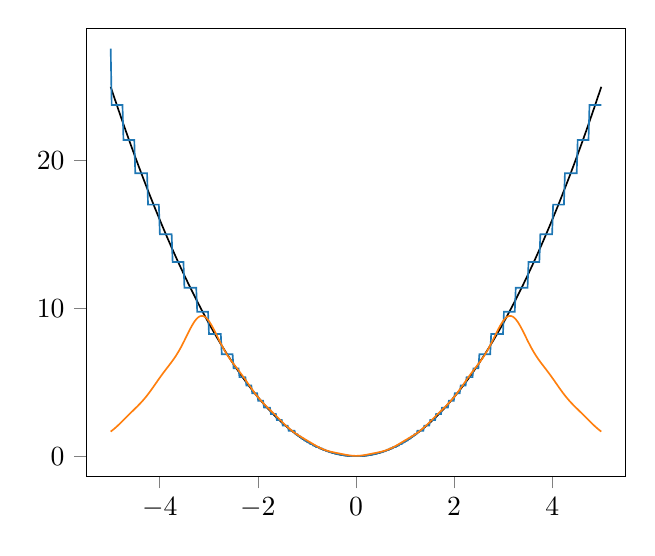
\begin{tikzpicture}

\definecolor{color0}{rgb}{0.12156862745098,0.466666666666667,0.705882352941177}
\definecolor{color1}{rgb}{1,0.498039215686275,0.0549019607843137}

\begin{axis}[
xmin=-5.5, xmax=5.5,
ymin=-1.37906124373759, ymax=28.9624949449599,
tick align=outside,
tick pos=left,
x grid style={white!69.01960784313725!black},
y grid style={white!69.01960784313725!black}
]
\addplot [semithick, black, forget plot]
table {%
-5 25
-4.97995991983968 24.8000008032096
-4.95991983967936 24.6008048160449
-4.93987975951904 24.4024120385059
-4.91983967935872 24.2048224705925
-4.8997995991984 24.0080361123048
-4.87975951903808 23.8120529636427
-4.85971943887776 23.6168730246063
-4.83967935871743 23.4224962951956
-4.81963927855711 23.2289227754105
-4.79959919839679 23.0361524652511
-4.77955911823647 22.8441853647174
-4.75951903807615 22.6530214738093
-4.73947895791583 22.4626607925269
-4.71943887775551 22.2731033208702
-4.69939879759519 22.0843490588391
-4.67935871743487 21.8963980064337
-4.65931863727455 21.709250163654
-4.63927855711423 21.5229055304999
-4.61923847695391 21.3373641069715
-4.59919839679359 21.1526258930687
-4.57915831663327 20.9686908887916
-4.55911823647295 20.7855590941402
-4.53907815631263 20.6032305091144
-4.51903807615231 20.4217051337143
-4.49899799599198 20.2409829679399
-4.47895791583166 20.0610640117911
-4.45891783567134 19.881948265268
-4.43887775551102 19.7036357283706
-4.4188376753507 19.5261264010988
-4.39879759519038 19.3494202834527
-4.37875751503006 19.1735173754322
-4.35871743486974 18.9984176770374
-4.33867735470942 18.8241211882683
-4.3186372745491 18.6506279091249
-4.29859719438878 18.4779378396071
-4.27855711422846 18.3060509797149
-4.25851703406814 18.1349673294485
-4.23847695390782 17.9646868888077
-4.2184368737475 17.7952096577925
-4.19839679358717 17.6265356364031
-4.17835671342685 17.4586648246393
-4.15831663326653 17.2915972225011
-4.13827655310621 17.1253328299886
-4.11823647294589 16.9598716471018
-4.09819639278557 16.7952136738407
-4.07815631262525 16.6313589102052
-4.05811623246493 16.4683073561954
-4.03807615230461 16.3060590118112
-4.01803607214429 16.1446138770527
-3.99799599198397 15.9839719519199
-3.97795591182365 15.8241332364127
-3.95791583166333 15.6650977305312
-3.93787575150301 15.5068654342754
-3.91783567134269 15.3494363476452
-3.89779559118236 15.1928104706407
-3.87775551102204 15.0369878032618
-3.85771543086172 14.8819683455087
-3.8376753507014 14.7277520973811
-3.81763527054108 14.5743390588793
-3.79759519038076 14.4217292300031
-3.77755511022044 14.2699226107526
-3.75751503006012 14.1189192011277
-3.7374749498998 13.9687190011285
-3.71743486973948 13.819322010755
-3.69739478957916 13.6707282300071
-3.67735470941884 13.5229376588849
-3.65731462925852 13.3759502973884
-3.6372745490982 13.2297661455175
-3.61723446893788 13.0843852032723
-3.59719438877756 12.9398074706527
-3.57715430861723 12.7960329476588
-3.55711422845691 12.6530616342906
-3.53707414829659 12.5108935305481
-3.51703406813627 12.3695286364312
-3.49699398797595 12.22896695194
-3.47695390781563 12.0892084770744
-3.45691382765531 11.9502532118345
-3.43687374749499 11.8121011562203
-3.41683366733467 11.6747523102317
-3.39679358717435 11.5382066738688
-3.37675350701403 11.4024642471315
-3.35671342685371 11.26752503002
-3.33667334669339 11.133389022534
-3.31663326653307 11.0000562246738
-3.29659318637275 10.8675266364392
-3.27655310621242 10.7358002578303
-3.2565130260521 10.604877088847
-3.23647294589178 10.4747571294894
-3.21643286573146 10.3454403797575
-3.19639278557114 10.2169268396512
-3.17635270541082 10.0892165091706
-3.1563126252505 9.96230938831571
-3.13627254509018 9.83620547708644
-3.11623246492986 9.71090477548283
-3.09619238476954 9.58640728350489
-3.07615230460922 9.4627130011526
-3.0561122244489 9.33982192842599
-3.03607214428858 9.21773406532504
-3.01603206412826 9.09644941184975
-2.99599198396794 8.97596796800013
-2.97595190380762 8.85628973377617
-2.95591182364729 8.73741470917788
-2.93587174348697 8.61934289420524
-2.91583166332665 8.50207428885828
-2.89579158316633 8.38560889313698
-2.87575150300601 8.26994670704134
-2.85571142284569 8.15508773057137
-2.83567134268537 8.04103196372705
-2.81563126252505 7.92777940650841
-2.79559118236473 7.81533005891543
-2.77555110220441 7.70368392094811
-2.75551102204409 7.59284099260646
-2.73547094188377 7.48280127389047
-2.71543086172345 7.37356476480014
-2.69539078156313 7.26513146533548
-2.67535070140281 7.15750137549648
-2.65531062124249 7.05067449528315
-2.63527054108216 6.94465082469548
-2.61523046092184 6.83943036373348
-2.59519038076152 6.73501311239714
-2.5751503006012 6.63139907068646
-2.55511022044088 6.52858823860145
-2.53507014028056 6.4265806161421
-2.51503006012024 6.32537620330842
-2.49498997995992 6.2249750001004
-2.4749498997996 6.12537700651805
-2.45490981963928 6.02658222256135
-2.43486973947896 5.92859064823033
-2.41482965931864 5.83140228352497
-2.39478957915832 5.73501712844527
-2.374749498998 5.63943518299123
-2.35470941883768 5.54465644716286
-2.33466933867735 5.45068092096016
-2.31462925851703 5.35750860438312
-2.29458917835671 5.26513949743174
-2.27454909819639 5.17357360010602
-2.25450901803607 5.08281091240598
-2.23446893787575 4.99285143433159
-2.21442885771543 4.90369516588287
-2.19438877755511 4.81534210705981
-2.17434869739479 4.72779225786242
-2.15430861723447 4.64104561829069
-2.13426853707415 4.55510218834462
-2.11422845691383 4.46996196802423
-2.09418837675351 4.38562495732949
-2.07414829659319 4.30209115626042
-2.05410821643287 4.21936056481701
-2.03406813627255 4.13743318299927
-2.01402805611222 4.05630901080719
-1.9939879759519 3.97598804824077
-1.97394789579158 3.89647029530002
-1.95390781563126 3.81775575198493
-1.93386773547094 3.73984441829551
-1.91382765531062 3.66273629423175
-1.8937875751503 3.58643137979366
-1.87374749498998 3.51092967498123
-1.85370741482966 3.43623117979446
-1.83366733466934 3.36233589423336
-1.81362725450902 3.28924381829792
-1.7935871743487 3.21695495198815
-1.77354709418838 3.14546929530404
-1.75350701402806 3.07478684824559
-1.73346693386774 3.00490761081281
-1.71342685370742 2.93583158300569
-1.69338677354709 2.86755876482424
-1.67334669338677 2.80008915626845
-1.65330661322645 2.73342275733832
-1.63326653306613 2.66755956803386
-1.61322645290581 2.60249958835507
-1.59318637274549 2.53824281830193
-1.57314629258517 2.47478925787447
-1.55310621242485 2.41213890707266
-1.53306613226453 2.35029176589652
-1.51302605210421 2.28924783434605
-1.49298597194389 2.22900711242124
-1.47294589178357 2.16956960012209
-1.45290581162325 2.11093529744861
-1.43286573146293 2.05310420440079
-1.41282565130261 1.99607632097863
-1.39278557114228 1.93985164718214
-1.37274549098196 1.88443018301131
-1.35270541082164 1.82981192846615
-1.33266533066132 1.77599688354665
-1.312625250501 1.72298504825282
-1.29258517034068 1.67077642258465
-1.27254509018036 1.61937100654214
-1.25250501002004 1.5687688001253
-1.23246492985972 1.51896980333412
-1.2124248496994 1.46997401616861
-1.19238476953908 1.42178143862876
-1.17234468937876 1.37439207071458
-1.15230460921844 1.32780591242605
-1.13226452905812 1.2820229637632
-1.1122244488978 1.23704322472601
-1.09218436873748 1.19286669531448
-1.07214428857715 1.14949337552861
-1.05210420841683 1.10692326536841
-1.03206412825651 1.06515636483388
-1.01202404809619 1.024192673925
-0.991983967935872 0.984032192641798
-0.971943887775551 0.944674920984253
-0.95190380761523 0.906120858952374
-0.93186372745491 0.86837000654616
-0.91182364729459 0.831422363765608
-0.891783567134269 0.795277930610721
-0.871743486973948 0.759936707081497
-0.851703406813628 0.72539869317794
-0.831663326653307 0.691663888900045
-0.811623246492986 0.658732294247814
-0.791583166332665 0.626603909221248
-0.771543086172345 0.595278733820347
-0.751503006012024 0.564756768045109
-0.731462925851703 0.535038011895534
-0.711422845691383 0.506122465371626
-0.691382765531062 0.47801012847338
-0.671342685370742 0.450701001200799
-0.651302605210421 0.424195083553881
-0.631262525050101 0.398492375532629
-0.61122244488978 0.37359287713704
-0.591182364729459 0.349496588367115
-0.571142284569138 0.326203509222854
-0.551102204408818 0.303713639704259
-0.531062124248497 0.282026979811326
-0.511022044088176 0.261143529544058
-0.490981963927856 0.241063288902455
-0.470941883767535 0.221786257886515
-0.450901803607215 0.203312436496239
-0.430861723446894 0.185641824731627
-0.410821643286574 0.168774422592681
-0.390781563126253 0.152710230079397
-0.370741482965932 0.137449247191778
-0.350701402805611 0.122991473929823
-0.330661322645291 0.109336910293533
-0.31062124248497 0.0964855562829066
-0.290581162324649 0.0844374118979442
-0.270541082164329 0.0731924771386464
-0.250501002004008 0.0627507520050122
-0.230460921843687 0.0531122364970422
-0.210420841683367 0.0442769306147364
-0.190380761523047 0.0362448343580951
-0.170340681362726 0.0290159477271177
-0.150300601202405 0.0225902707218043
-0.130260521042084 0.0169678033421552
-0.110220440881764 0.0121485455881704
-0.0901803607214431 0.00813249745984959
-0.0701402805611222 0.00491965895719294
-0.0501002004008022 0.00251003008020054
-0.0300601202404813 0.000903610828872195
-0.0100200400801604 0.000100401203208022
0.0100200400801604 0.000100401203208022
0.0300601202404804 0.000903610828872142
0.0501002004008013 0.00251003008020045
0.0701402805611222 0.00491965895719294
0.0901803607214431 0.00813249745984959
0.110220440881763 0.0121485455881702
0.130260521042084 0.0169678033421552
0.150300601202405 0.0225902707218043
0.170340681362725 0.0290159477271174
0.190380761523046 0.0362448343580948
0.210420841683367 0.0442769306147364
0.230460921843687 0.0531122364970422
0.250501002004007 0.0627507520050118
0.270541082164328 0.0731924771386459
0.290581162324649 0.0844374118979442
0.31062124248497 0.0964855562829066
0.33066132264529 0.109336910293533
0.350701402805611 0.122991473929823
0.370741482965932 0.137449247191778
0.390781563126252 0.152710230079397
0.410821643286573 0.16877442259268
0.430861723446894 0.185641824731627
0.450901803607215 0.203312436496239
0.470941883767535 0.221786257886514
0.490981963927855 0.241063288902454
0.511022044088176 0.261143529544058
0.531062124248497 0.282026979811326
0.551102204408817 0.303713639704258
0.571142284569138 0.326203509222854
0.591182364729459 0.349496588367115
0.611222444889779 0.373592877137039
0.6312625250501 0.398492375532628
0.651302605210421 0.424195083553881
0.671342685370742 0.450701001200799
0.691382765531062 0.478010128473379
0.711422845691382 0.506122465371625
0.731462925851703 0.535038011895534
0.751503006012024 0.564756768045109
0.771543086172344 0.595278733820345
0.791583166332665 0.626603909221248
0.811623246492986 0.658732294247814
0.831663326653306 0.691663888900044
0.851703406813627 0.725398693177938
0.871743486973948 0.759936707081497
0.891783567134269 0.795277930610721
0.911823647294589 0.831422363765606
0.93186372745491 0.868370006546158
0.95190380761523 0.906120858952374
0.971943887775551 0.944674920984253
0.991983967935871 0.984032192641796
1.01202404809619 1.024192673925
1.03206412825651 1.06515636483388
1.05210420841683 1.10692326536841
1.07214428857715 1.14949337552861
1.09218436873747 1.19286669531448
1.1122244488978 1.23704322472601
1.13226452905812 1.2820229637632
1.15230460921844 1.32780591242605
1.17234468937876 1.37439207071458
1.19238476953908 1.42178143862876
1.2124248496994 1.46997401616861
1.23246492985972 1.51896980333412
1.25250501002004 1.5687688001253
1.27254509018036 1.61937100654214
1.29258517034068 1.67077642258465
1.312625250501 1.72298504825282
1.33266533066132 1.77599688354665
1.35270541082164 1.82981192846615
1.37274549098196 1.88443018301131
1.39278557114228 1.93985164718214
1.4128256513026 1.99607632097863
1.43286573146293 2.05310420440078
1.45290581162325 2.1109352974486
1.47294589178357 2.16956960012209
1.49298597194389 2.22900711242123
1.51302605210421 2.28924783434605
1.53306613226453 2.35029176589652
1.55310621242485 2.41213890707266
1.57314629258517 2.47478925787446
1.59318637274549 2.53824281830193
1.61322645290581 2.60249958835507
1.63326653306613 2.66755956803386
1.65330661322645 2.73342275733832
1.67334669338677 2.80008915626845
1.69338677354709 2.86755876482424
1.71342685370741 2.93583158300569
1.73346693386774 3.00490761081281
1.75350701402806 3.07478684824559
1.77354709418838 3.14546929530404
1.7935871743487 3.21695495198814
1.81362725450902 3.28924381829792
1.83366733466934 3.36233589423336
1.85370741482966 3.43623117979446
1.87374749498998 3.51092967498122
1.8937875751503 3.58643137979365
1.91382765531062 3.66273629423175
1.93386773547094 3.73984441829551
1.95390781563126 3.81775575198493
1.97394789579158 3.89647029530002
1.9939879759519 3.97598804824077
2.01402805611222 4.05630901080718
2.03406813627254 4.13743318299926
2.05410821643287 4.21936056481701
2.07414829659319 4.30209115626041
2.09418837675351 4.38562495732949
2.11422845691383 4.46996196802422
2.13426853707415 4.55510218834462
2.15430861723447 4.64104561829069
2.17434869739479 4.72779225786242
2.19438877755511 4.81534210705981
2.21442885771543 4.90369516588287
2.23446893787575 4.99285143433159
2.25450901803607 5.08281091240597
2.27454909819639 5.17357360010602
2.29458917835671 5.26513949743173
2.31462925851703 5.35750860438311
2.33466933867735 5.45068092096016
2.35470941883768 5.54465644716286
2.374749498998 5.63943518299123
2.39478957915832 5.73501712844527
2.41482965931864 5.83140228352497
2.43486973947896 5.92859064823033
2.45490981963928 6.02658222256135
2.4749498997996 6.12537700651804
2.49498997995992 6.2249750001004
2.51503006012024 6.32537620330842
2.53507014028056 6.4265806161421
2.55511022044088 6.52858823860145
2.5751503006012 6.63139907068646
2.59519038076152 6.73501311239714
2.61523046092184 6.83943036373348
2.63527054108216 6.94465082469548
2.65531062124249 7.05067449528315
2.67535070140281 7.15750137549648
2.69539078156313 7.26513146533548
2.71543086172345 7.37356476480014
2.73547094188377 7.48280127389046
2.75551102204409 7.59284099260645
2.77555110220441 7.70368392094811
2.79559118236473 7.81533005891543
2.81563126252505 7.9277794065084
2.83567134268537 8.04103196372705
2.85571142284569 8.15508773057136
2.87575150300601 8.26994670704134
2.89579158316633 8.38560889313697
2.91583166332665 8.50207428885828
2.93587174348697 8.61934289420524
2.95591182364729 8.73741470917787
2.97595190380761 8.85628973377617
2.99599198396794 8.97596796800013
3.01603206412826 9.09644941184975
3.03607214428858 9.21773406532503
3.0561122244489 9.33982192842599
3.07615230460922 9.4627130011526
3.09619238476954 9.58640728350489
3.11623246492986 9.71090477548283
3.13627254509018 9.83620547708643
3.1563126252505 9.9623093883157
3.17635270541082 10.0892165091706
3.19639278557114 10.2169268396512
3.21643286573146 10.3454403797575
3.23647294589178 10.4747571294894
3.2565130260521 10.604877088847
3.27655310621243 10.7358002578303
3.29659318637274 10.8675266364392
3.31663326653307 11.0000562246738
3.33667334669339 11.133389022534
3.35671342685371 11.26752503002
3.37675350701403 11.4024642471315
3.39679358717435 11.5382066738688
3.41683366733467 11.6747523102317
3.43687374749499 11.8121011562202
3.45691382765531 11.9502532118345
3.47695390781563 12.0892084770744
3.49699398797595 12.2289669519399
3.51703406813627 12.3695286364312
3.53707414829659 12.5108935305481
3.55711422845691 12.6530616342906
3.57715430861723 12.7960329476588
3.59719438877755 12.9398074706527
3.61723446893788 13.0843852032723
3.6372745490982 13.2297661455175
3.65731462925852 13.3759502973884
3.67735470941884 13.5229376588849
3.69739478957916 13.6707282300071
3.71743486973948 13.819322010755
3.7374749498998 13.9687190011285
3.75751503006012 14.1189192011277
3.77755511022044 14.2699226107526
3.79759519038076 14.4217292300031
3.81763527054108 14.5743390588793
3.8376753507014 14.7277520973811
3.85771543086172 14.8819683455087
3.87775551102204 15.0369878032618
3.89779559118236 15.1928104706407
3.91783567134268 15.3494363476452
3.93787575150301 15.5068654342754
3.95791583166333 15.6650977305312
3.97795591182365 15.8241332364127
3.99799599198397 15.9839719519199
4.01803607214429 16.1446138770527
4.03807615230461 16.3060590118112
4.05811623246493 16.4683073561953
4.07815631262525 16.6313589102052
4.09819639278557 16.7952136738407
4.11823647294589 16.9598716471018
4.13827655310621 17.1253328299886
4.15831663326653 17.2915972225011
4.17835671342685 17.4586648246392
4.19839679358717 17.6265356364031
4.21843687374749 17.7952096577925
4.23847695390782 17.9646868888077
4.25851703406814 18.1349673294485
4.27855711422846 18.3060509797149
4.29859719438878 18.4779378396071
4.3186372745491 18.6506279091249
4.33867735470942 18.8241211882683
4.35871743486974 18.9984176770374
4.37875751503006 19.1735173754322
4.39879759519038 19.3494202834527
4.4188376753507 19.5261264010988
4.43887775551102 19.7036357283706
4.45891783567134 19.881948265268
4.47895791583166 20.0610640117911
4.49899799599198 20.2409829679399
4.5190380761523 20.4217051337143
4.53907815631263 20.6032305091144
4.55911823647295 20.7855590941402
4.57915831663327 20.9686908887916
4.59919839679359 21.1526258930687
4.61923847695391 21.3373641069714
4.63927855711423 21.5229055304999
4.65931863727455 21.709250163654
4.67935871743487 21.8963980064337
4.69939879759519 22.0843490588391
4.71943887775551 22.2731033208702
4.73947895791583 22.4626607925269
4.75951903807615 22.6530214738093
4.77955911823647 22.8441853647174
4.79959919839679 23.0361524652511
4.81963927855711 23.2289227754105
4.83967935871743 23.4224962951956
4.85971943887776 23.6168730246063
4.87975951903808 23.8120529636427
4.8997995991984 24.0080361123048
4.91983967935872 24.2048224705925
4.93987975951904 24.4024120385059
4.95991983967936 24.6008048160449
4.97995991983968 24.8000008032096
5 25
};
\addplot [semithick, color0, forget plot]
table {%
-5 27.5833333000191
-4.97995991983968 23.7708333000191
-4.95991983967936 23.7708333000191
-4.93987975951904 23.7708333000191
-4.91983967935872 23.7708333000191
-4.8997995991984 23.7708333000191
-4.87975951903808 23.7708333000191
-4.85971943887776 23.7708333000191
-4.83967935871743 23.7708333000191
-4.81963927855711 23.7708333000191
-4.79959919839679 23.7708333000191
-4.77955911823647 23.7708333000191
-4.75951903807615 23.7708333000191
-4.73947895791583 21.3958333000191
-4.71943887775551 21.3958333000191
-4.69939879759519 21.3958333000191
-4.67935871743487 21.3958333000191
-4.65931863727455 21.3958333000191
-4.63927855711423 21.3958333000191
-4.61923847695391 21.3958333000191
-4.59919839679359 21.3958333000191
-4.57915831663327 21.3958333000191
-4.55911823647295 21.3958333000191
-4.53907815631263 21.3958333000191
-4.51903807615231 21.3958333000191
-4.49899799599198 19.1458333000191
-4.47895791583166 19.1458333000191
-4.45891783567134 19.1458333000191
-4.43887775551102 19.1458333000191
-4.4188376753507 19.1458333000191
-4.39879759519038 19.1458333000191
-4.37875751503006 19.1458333000191
-4.35871743486974 19.1458333000191
-4.33867735470942 19.1458333000191
-4.3186372745491 19.1458333000191
-4.29859719438878 19.1458333000191
-4.27855711422846 19.1458333000191
-4.25851703406814 19.1458333000191
-4.23847695390782 17.0208333000191
-4.2184368737475 17.0208333000191
-4.19839679358717 17.0208333000191
-4.17835671342685 17.0208333000191
-4.15831663326653 17.0208333000191
-4.13827655310621 17.0208333000191
-4.11823647294589 17.0208333000191
-4.09819639278557 17.0208333000191
-4.07815631262525 17.0208333000191
-4.05811623246493 17.0208333000191
-4.03807615230461 17.0208333000191
-4.01803607214429 17.0208333000191
-3.99799599198397 15.0208333000191
-3.97795591182365 15.0208333000191
-3.95791583166333 15.0208333000191
-3.93787575150301 15.0208333000191
-3.91783567134269 15.0208333000191
-3.89779559118236 15.0208333000191
-3.87775551102204 15.0208333000191
-3.85771543086172 15.0208333000191
-3.8376753507014 15.0208333000191
-3.81763527054108 15.0208333000191
-3.79759519038076 15.0208333000191
-3.77755511022044 15.0208333000191
-3.75751503006012 15.0208333000191
-3.7374749498998 13.1458333000191
-3.71743486973948 13.1458333000191
-3.69739478957916 13.1458333000191
-3.67735470941884 13.1458333000191
-3.65731462925852 13.1458333000191
-3.6372745490982 13.1458333000191
-3.61723446893788 13.1458333000191
-3.59719438877756 13.1458333000191
-3.57715430861723 13.1458333000191
-3.55711422845691 13.1458333000191
-3.53707414829659 13.1458333000191
-3.51703406813627 13.1458333000191
-3.49699398797595 11.3958333000191
-3.47695390781563 11.3958333000191
-3.45691382765531 11.3958333000191
-3.43687374749499 11.3958333000191
-3.41683366733467 11.3958333000191
-3.39679358717435 11.3958333000191
-3.37675350701403 11.3958333000191
-3.35671342685371 11.3958333000191
-3.33667334669339 11.3958333000191
-3.31663326653307 11.3958333000191
-3.29659318637275 11.3958333000191
-3.27655310621242 11.3958333000191
-3.2565130260521 11.3958333000191
-3.23647294589178 9.77083330001915
-3.21643286573146 9.77083330001915
-3.19639278557114 9.77083330001915
-3.17635270541082 9.77083330001915
-3.1563126252505 9.77083330001915
-3.13627254509018 9.77083330001915
-3.11623246492986 9.77083330001915
-3.09619238476954 9.77083330001915
-3.07615230460922 9.77083330001915
-3.0561122244489 9.77083330001915
-3.03607214428858 9.77083330001915
-3.01603206412826 9.77083330001915
-2.99599198396794 8.27083330001915
-2.97595190380762 8.27083330001915
-2.95591182364729 8.27083330001915
-2.93587174348697 8.27083330001915
-2.91583166332665 8.27083330001915
-2.89579158316633 8.27083330001915
-2.87575150300601 8.27083330001915
-2.85571142284569 8.27083330001915
-2.83567134268537 8.27083330001915
-2.81563126252505 8.27083330001915
-2.79559118236473 8.27083330001915
-2.77555110220441 8.27083330001915
-2.75551102204409 8.27083330001915
-2.73547094188377 6.89583330001915
-2.71543086172345 6.89583330001915
-2.69539078156313 6.89583330001915
-2.67535070140281 6.89583330001915
-2.65531062124249 6.89583330001915
-2.63527054108216 6.89583330001915
-2.61523046092184 6.89583330001915
-2.59519038076152 6.89583330001915
-2.5751503006012 6.89583330001915
-2.55511022044088 6.89583330001915
-2.53507014028056 6.89583330001915
-2.51503006012024 6.89583330001915
-2.49498997995992 5.94270830001915
-2.4749498997996 5.94270830001915
-2.45490981963928 5.94270830001915
-2.43486973947896 5.94270830001915
-2.41482965931864 5.94270830001915
-2.39478957915832 5.94270830001915
-2.374749498998 5.34895830001915
-2.35470941883768 5.34895830001915
-2.33466933867735 5.34895830001915
-2.31462925851703 5.34895830001915
-2.29458917835671 5.34895830001915
-2.27454909819639 5.34895830001915
-2.25450901803607 5.34895830001915
-2.23446893787575 4.78645830001915
-2.21442885771543 4.78645830001915
-2.19438877755511 4.78645830001915
-2.17434869739479 4.78645830001915
-2.15430861723447 4.78645830001915
-2.13426853707415 4.78645830001915
-2.11422845691383 4.25520830001915
-2.09418837675351 4.25520830001915
-2.07414829659319 4.25520830001915
-2.05410821643287 4.25520830001915
-2.03406813627255 4.25520830001915
-2.01402805611222 4.25520830001915
-1.9939879759519 3.75520830001915
-1.97394789579158 3.75520830001915
-1.95390781563126 3.75520830001915
-1.93386773547094 3.75520830001915
-1.91382765531062 3.75520830001915
-1.8937875751503 3.75520830001915
-1.87374749498998 3.28645830001915
-1.85370741482966 3.28645830001915
-1.83366733466934 3.28645830001915
-1.81362725450902 3.28645830001915
-1.7935871743487 3.28645830001915
-1.77354709418838 3.28645830001915
-1.75350701402806 3.28645830001915
-1.73346693386774 2.84895830001915
-1.71342685370742 2.84895830001915
-1.69338677354709 2.84895830001915
-1.67334669338677 2.84895830001915
-1.65330661322645 2.84895830001915
-1.63326653306613 2.84895830001915
-1.61322645290581 2.44270830001915
-1.59318637274549 2.44270830001915
-1.57314629258517 2.44270830001915
-1.55310621242485 2.44270830001915
-1.53306613226453 2.44270830001915
-1.51302605210421 2.44270830001915
-1.49298597194389 2.06770830001915
-1.47294589178357 2.06770830001915
-1.45290581162325 2.06770830001915
-1.43286573146293 2.06770830001915
-1.41282565130261 2.06770830001915
-1.39278557114228 2.06770830001915
-1.37274549098196 1.72395830001915
-1.35270541082164 1.72395830001915
-1.33266533066132 1.72395830001915
-1.312625250501 1.72395830001915
-1.29258517034068 1.72395830001915
-1.27254509018036 1.72395830001915
-1.25250501002004 1.72395830001915
-1.23246492985972 1.48567705001915
-1.2124248496994 1.48567705001915
-1.19238476953908 1.48567705001915
-1.17234468937876 1.33723955001915
-1.15230460921844 1.33723955001915
-1.13226452905812 1.33723955001915
-1.1122244488978 1.19661455001915
-1.09218436873748 1.19661455001915
-1.07214428857715 1.19661455001915
-1.05210420841683 1.06380205001915
-1.03206412825651 1.06380205001915
-1.01202404809619 1.06380205001915
-0.991983967935872 0.938802050019149
-0.971943887775551 0.938802050019149
-0.95190380761523 0.938802050019149
-0.93186372745491 0.821614550019149
-0.91182364729459 0.821614550019149
-0.891783567134269 0.821614550019149
-0.871743486973948 0.712239550019149
-0.851703406813628 0.712239550019149
-0.831663326653307 0.712239550019149
-0.811623246492986 0.610677050019149
-0.791583166332665 0.610677050019149
-0.771543086172345 0.610677050019149
-0.751503006012024 0.610677050019149
-0.731462925851703 0.516927050019149
-0.711422845691383 0.516927050019149
-0.691382765531062 0.516927050019149
-0.671342685370742 0.430989550019149
-0.651302605210421 0.430989550019149
-0.631262525050101 0.430989550019149
-0.61122244488978 0.371419237519149
-0.591182364729459 0.334309862519149
-0.571142284569138 0.334309862519149
-0.551102204408818 0.299153612519149
-0.531062124248497 0.265950487519149
-0.511022044088176 0.265950487519149
-0.490981963927856 0.234700487519149
-0.470941883767535 0.234700487519149
-0.450901803607215 0.205403612519149
-0.430861723446894 0.178059862519149
-0.410821643286574 0.178059862519149
-0.390781563126253 0.152669237519149
-0.370741482965932 0.129231737519149
-0.350701402805611 0.129231737519149
-0.330661322645291 0.107747362519149
-0.31062124248497 0.0928547843941487
-0.290581162324649 0.0835774406441487
-0.270541082164329 0.0747883781441487
-0.250501002004008 0.0664875968941487
-0.230460921843687 0.0513508781441487
-0.210420841683367 0.0445149406441487
-0.190380761523047 0.0381672843941487
-0.170340681362726 0.0269368156441487
-0.150300601202405 0.0232136711128987
-0.130260521042084 0.0166218742378987
-0.110220440881764 0.0128376945503987
-0.0901803607214431 0.00807695236289874
-0.0701402805611222 0.00467424240196124
-0.0501002004008022 0.00238542404258624
-0.0300601202404813 0.000916765595320612
-0.0100200400801604 0.000105188752058893
0.0100200400801604 0.000105188752058893
0.0300601202404804 0.000916765595320612
0.0501002004008013 0.00238542404258624
0.0701402805611222 0.00467424240196124
0.0901803607214431 0.00807695236289874
0.110220440881763 0.0128376945503987
0.130260521042084 0.0166218742378987
0.150300601202405 0.0232136711128987
0.170340681362725 0.0269368156441487
0.190380761523046 0.0381672843941487
0.210420841683367 0.0445149406441487
0.230460921843687 0.0513508781441487
0.250501002004007 0.0664875968941487
0.270541082164328 0.0747883781441487
0.290581162324649 0.0835774406441487
0.31062124248497 0.0928547843941487
0.33066132264529 0.107747362519149
0.350701402805611 0.129231737519149
0.370741482965932 0.129231737519149
0.390781563126252 0.152669237519149
0.410821643286573 0.178059862519149
0.430861723446894 0.178059862519149
0.450901803607215 0.205403612519149
0.470941883767535 0.234700487519149
0.490981963927855 0.234700487519149
0.511022044088176 0.265950487519149
0.531062124248497 0.265950487519149
0.551102204408817 0.299153612519149
0.571142284569138 0.334309862519149
0.591182364729459 0.334309862519149
0.611222444889779 0.371419237519149
0.6312625250501 0.430989550019149
0.651302605210421 0.430989550019149
0.671342685370742 0.430989550019149
0.691382765531062 0.516927050019149
0.711422845691382 0.516927050019149
0.731462925851703 0.516927050019149
0.751503006012024 0.610677050019149
0.771543086172344 0.610677050019149
0.791583166332665 0.610677050019149
0.811623246492986 0.610677050019149
0.831663326653306 0.712239550019149
0.851703406813627 0.712239550019149
0.871743486973948 0.712239550019149
0.891783567134269 0.821614550019149
0.911823647294589 0.821614550019149
0.93186372745491 0.821614550019149
0.95190380761523 0.938802050019149
0.971943887775551 0.938802050019149
0.991983967935871 0.938802050019149
1.01202404809619 1.06380205001915
1.03206412825651 1.06380205001915
1.05210420841683 1.06380205001915
1.07214428857715 1.19661455001915
1.09218436873747 1.19661455001915
1.1122244488978 1.19661455001915
1.13226452905812 1.33723955001915
1.15230460921844 1.33723955001915
1.17234468937876 1.33723955001915
1.19238476953908 1.48567705001915
1.2124248496994 1.48567705001915
1.23246492985972 1.48567705001915
1.25250501002004 1.72395830001915
1.27254509018036 1.72395830001915
1.29258517034068 1.72395830001915
1.312625250501 1.72395830001915
1.33266533066132 1.72395830001915
1.35270541082164 1.72395830001915
1.37274549098196 1.72395830001915
1.39278557114228 2.06770830001915
1.4128256513026 2.06770830001915
1.43286573146293 2.06770830001915
1.45290581162325 2.06770830001915
1.47294589178357 2.06770830001915
1.49298597194389 2.06770830001915
1.51302605210421 2.44270830001915
1.53306613226453 2.44270830001915
1.55310621242485 2.44270830001915
1.57314629258517 2.44270830001915
1.59318637274549 2.44270830001915
1.61322645290581 2.44270830001915
1.63326653306613 2.84895830001915
1.65330661322645 2.84895830001915
1.67334669338677 2.84895830001915
1.69338677354709 2.84895830001915
1.71342685370741 2.84895830001915
1.73346693386774 2.84895830001915
1.75350701402806 3.28645830001915
1.77354709418838 3.28645830001915
1.7935871743487 3.28645830001915
1.81362725450902 3.28645830001915
1.83366733466934 3.28645830001915
1.85370741482966 3.28645830001915
1.87374749498998 3.28645830001915
1.8937875751503 3.75520830001915
1.91382765531062 3.75520830001915
1.93386773547094 3.75520830001915
1.95390781563126 3.75520830001915
1.97394789579158 3.75520830001915
1.9939879759519 3.75520830001915
2.01402805611222 4.25520830001915
2.03406813627254 4.25520830001915
2.05410821643287 4.25520830001915
2.07414829659319 4.25520830001915
2.09418837675351 4.25520830001915
2.11422845691383 4.25520830001915
2.13426853707415 4.78645830001915
2.15430861723447 4.78645830001915
2.17434869739479 4.78645830001915
2.19438877755511 4.78645830001915
2.21442885771543 4.78645830001915
2.23446893787575 4.78645830001915
2.25450901803607 5.34895830001915
2.27454909819639 5.34895830001915
2.29458917835671 5.34895830001915
2.31462925851703 5.34895830001915
2.33466933867735 5.34895830001915
2.35470941883768 5.34895830001915
2.374749498998 5.34895830001915
2.39478957915832 5.94270830001915
2.41482965931864 5.94270830001915
2.43486973947896 5.94270830001915
2.45490981963928 5.94270830001915
2.4749498997996 5.94270830001915
2.49498997995992 5.94270830001915
2.51503006012024 6.89583330001915
2.53507014028056 6.89583330001915
2.55511022044088 6.89583330001915
2.5751503006012 6.89583330001915
2.59519038076152 6.89583330001915
2.61523046092184 6.89583330001915
2.63527054108216 6.89583330001915
2.65531062124249 6.89583330001915
2.67535070140281 6.89583330001915
2.69539078156313 6.89583330001915
2.71543086172345 6.89583330001915
2.73547094188377 6.89583330001915
2.75551102204409 8.27083330001915
2.77555110220441 8.27083330001915
2.79559118236473 8.27083330001915
2.81563126252505 8.27083330001915
2.83567134268537 8.27083330001915
2.85571142284569 8.27083330001915
2.87575150300601 8.27083330001915
2.89579158316633 8.27083330001915
2.91583166332665 8.27083330001915
2.93587174348697 8.27083330001915
2.95591182364729 8.27083330001915
2.97595190380761 8.27083330001915
2.99599198396794 8.27083330001915
3.01603206412826 9.77083330001915
3.03607214428858 9.77083330001915
3.0561122244489 9.77083330001915
3.07615230460922 9.77083330001915
3.09619238476954 9.77083330001915
3.11623246492986 9.77083330001915
3.13627254509018 9.77083330001915
3.1563126252505 9.77083330001915
3.17635270541082 9.77083330001915
3.19639278557114 9.77083330001915
3.21643286573146 9.77083330001915
3.23647294589178 9.77083330001915
3.2565130260521 11.3958333000191
3.27655310621243 11.3958333000191
3.29659318637274 11.3958333000191
3.31663326653307 11.3958333000191
3.33667334669339 11.3958333000191
3.35671342685371 11.3958333000191
3.37675350701403 11.3958333000191
3.39679358717435 11.3958333000191
3.41683366733467 11.3958333000191
3.43687374749499 11.3958333000191
3.45691382765531 11.3958333000191
3.47695390781563 11.3958333000191
3.49699398797595 11.3958333000191
3.51703406813627 13.1458333000191
3.53707414829659 13.1458333000191
3.55711422845691 13.1458333000191
3.57715430861723 13.1458333000191
3.59719438877755 13.1458333000191
3.61723446893788 13.1458333000191
3.6372745490982 13.1458333000191
3.65731462925852 13.1458333000191
3.67735470941884 13.1458333000191
3.69739478957916 13.1458333000191
3.71743486973948 13.1458333000191
3.7374749498998 13.1458333000191
3.75751503006012 15.0208333000191
3.77755511022044 15.0208333000191
3.79759519038076 15.0208333000191
3.81763527054108 15.0208333000191
3.8376753507014 15.0208333000191
3.85771543086172 15.0208333000191
3.87775551102204 15.0208333000191
3.89779559118236 15.0208333000191
3.91783567134268 15.0208333000191
3.93787575150301 15.0208333000191
3.95791583166333 15.0208333000191
3.97795591182365 15.0208333000191
3.99799599198397 15.0208333000191
4.01803607214429 17.0208333000191
4.03807615230461 17.0208333000191
4.05811623246493 17.0208333000191
4.07815631262525 17.0208333000191
4.09819639278557 17.0208333000191
4.11823647294589 17.0208333000191
4.13827655310621 17.0208333000191
4.15831663326653 17.0208333000191
4.17835671342685 17.0208333000191
4.19839679358717 17.0208333000191
4.21843687374749 17.0208333000191
4.23847695390782 17.0208333000191
4.25851703406814 19.1458333000191
4.27855711422846 19.1458333000191
4.29859719438878 19.1458333000191
4.3186372745491 19.1458333000191
4.33867735470942 19.1458333000191
4.35871743486974 19.1458333000191
4.37875751503006 19.1458333000191
4.39879759519038 19.1458333000191
4.4188376753507 19.1458333000191
4.43887775551102 19.1458333000191
4.45891783567134 19.1458333000191
4.47895791583166 19.1458333000191
4.49899799599198 19.1458333000191
4.5190380761523 21.3958333000191
4.53907815631263 21.3958333000191
4.55911823647295 21.3958333000191
4.57915831663327 21.3958333000191
4.59919839679359 21.3958333000191
4.61923847695391 21.3958333000191
4.63927855711423 21.3958333000191
4.65931863727455 21.3958333000191
4.67935871743487 21.3958333000191
4.69939879759519 21.3958333000191
4.71943887775551 21.3958333000191
4.73947895791583 21.3958333000191
4.75951903807615 23.7708333000191
4.77955911823647 23.7708333000191
4.79959919839679 23.7708333000191
4.81963927855711 23.7708333000191
4.83967935871743 23.7708333000191
4.85971943887776 23.7708333000191
4.87975951903808 23.7708333000191
4.8997995991984 23.7708333000191
4.91983967935872 23.7708333000191
4.93987975951904 23.7708333000191
4.95991983967936 23.7708333000191
4.97995991983968 23.7708333000191
5 23.7708333000191
};
\addplot [semithick, color1, forget plot]
table {%
-5 1.66396458711919
-4.97995991983968 1.71453922572911
-4.95991983967936 1.76690695928443
-4.93987975951904 1.82109286031327
-4.91983967935872 1.87708553015322
-4.8997995991984 1.93483692950566
-4.87975951903808 1.99426351320675
-4.85971943887776 2.05524864970308
-4.83967935871743 2.1176462604606
-4.81963927855711 2.18128557084426
-4.79959919839679 2.24597682340377
-4.77955911823647 2.31151776842822
-4.75951903807615 2.37770071639281
-4.73947895791583 2.4443199136389
-4.71943887775551 2.51117898720846
-4.69939879759519 2.57809819784556
-4.67935871743487 2.64492124215279
-4.65931863727455 2.71152135582543
-4.63927855711423 2.77780648955439
-4.61923847695391 2.8437233570675
-4.59919839679359 2.90926019005695
-4.57915831663327 2.97444807634802
-4.55911823647295 3.03936080429808
-4.53907815631263 3.10411318658443
-4.51903807615231 3.1688578886093
-4.49899799599198 3.23378083899441
-4.47895791583166 3.2990953502958
-4.45891783567134 3.36503512540381
-4.43887775551102 3.43184636744661
-4.4188376753507 3.49977924686853
-4.39879759519038 3.56907900737622
-4.37875751503006 3.6399770115416
-4.35871743486974 3.71268203620277
-4.33867735470942 3.7873721269001
-4.3186372745491 3.86418730924393
-4.29859719438878 3.94322343348886
-4.27855711422846 4.02452739718755
-4.25851703406814 4.10809395044178
-4.23847695390782 4.19386424009804
-4.2184368737475 4.28172619466246
-4.19839679358717 4.37151679238417
-4.17835671342685 4.46302619271332
-4.15831663326653 4.55600364814373
-4.13827655310621 4.65016505133518
-4.11823647294589 4.74520191341453
-4.09819639278557 4.84079151545623
-4.07815631262525 4.93660792819375
-4.05811623246493 5.03233355668142
-4.03807615230461 5.12767083833452
-4.01803607214429 5.22235370565862
-3.99799599198397 5.31615841983643
-3.97795591182365 5.40891338861099
-3.95791583166333 5.50050760164199
-3.93787575150301 5.59089734838322
-3.91783567134269 5.68011092681004
-3.89779559118236 5.7682511049269
-3.87775551102204 5.85549515947041
-3.85771543086172 5.94209238585922
-3.8376753507014 6.02835904823792
-3.81763527054108 6.11467081623358
-3.79759519038076 6.20145281347515
-3.77755511022044 6.28916747964127
-3.75751503006012 6.37830052043288
-3.7374749498998 6.46934528613353
-3.71743486973948 6.56278597719137
-3.69739478957916 6.65908012262822
-3.67735470941884 6.75864081242796
-3.65731462925852 6.86181918709183
-3.6372745490982 6.96888769536339
-3.61723446893788 7.08002462422521
-3.59719438877756 7.19530038358711
-3.57715430861723 7.31466599199803
-3.55711422845691 7.43794416002638
-3.53707414829659 7.56482330588974
-3.51703406813627 7.69485476507572
-3.49699398797595 7.82745337402406
-3.47695390781563 7.96190151965863
-3.45691382765531 8.09735665411367
-3.43687374749499 8.23286217998363
-3.41683366733467 8.36736151851073
-3.39679358717435 8.49971508397215
-3.37675350701403 8.62871980472114
-3.35671342685371 8.75313075729476
-3.33667334669339 8.87168441691476
-3.31663326653307 8.98312297746725
-3.29659318637275 9.08621915818717
-3.27655310621242 9.17980089392549
-3.2565130260521 9.26277530173549
-3.23647294589178 9.33415132880924
-3.21643286573146 9.39306051529104
-3.19639278557114 9.43877534948589
-3.17635270541082 9.47072475132038
-3.1563126252505 9.48850629103615
-3.13627254509018 9.49189483206934
-3.11623246492986 9.48084737764553
-3.09619238476954 9.45550399730083
-3.07615230460922 9.41618480965166
-3.0561122244489 9.36338309850423
-3.03607214428858 9.29775473802608
-3.01603206412826 9.22010419646509
-2.99599198396794 9.13136747420681
-2.97595190380762 9.03259240843433
-2.95591182364729 8.92491684120867
-2.93587174348697 8.80954519867856
-2.91583166332665 8.68772406500744
-2.89579158316633 8.56071735455772
-2.87575150300601 8.42978168944003
-2.85571142284569 8.29614257673025
-2.83567134268537 8.16097195095825
-2.81563126252505 8.02536760380959
-2.79559118236473 7.89033496570529
-2.77555110220441 7.75677163476622
-2.75551102204409 7.62545496968342
-2.73547094188377 7.49703297652646
-2.71543086172345 7.37201862804285
-2.69539078156313 7.25078766016856
-2.67535070140281 7.13357979695951
-2.65531062124249 7.02050326460434
-2.63527054108216 6.91154237011471
-2.61523046092184 6.8065678430472
-2.59519038076152 6.70534957127128
-2.5751503006012 6.60757130612889
-2.55511022044088 6.51284686973849
-2.53507014028056 6.42073736868347
-2.51503006012024 6.33076890447254
-2.49498997995992 6.24245027210772
-2.4749498997996 6.15529015354988
-2.45490981963928 6.06881334211253
-2.43486973947896 5.98257557572893
-2.41482965931864 5.89617661015211
-2.39478957915832 5.80927122568189
-2.374749498998 5.72157793093524
-2.35470941883768 5.63288520226719
-2.33466933867735 5.54305517537274
-2.31462925851703 5.45202478397527
-2.29458917835671 5.35980441698031
-2.27454909819639 5.26647423779032
-2.25450901803607 5.17217837554873
-2.23446893787575 5.07711725604753
-2.21442885771543 4.98153838831216
-2.19438877755511 4.88572596021317
-2.17434869739479 4.78998962194891
-2.15430861723447 4.69465284937876
-2.13426853707415 4.60004127983472
-2.11422845691383 4.50647140146064
-2.09418837675351 4.41423995395652
-2.07414829659319 4.3236143648223
-2.05410821643287 4.23482450209412
-2.03406813627255 4.14805597370659
-2.01402805611222 4.06344514676929
-1.9939879759519 3.9810759991424
-1.97394789579158 3.90097885275207
-1.95390781563126 3.82313097514582
-1.93386773547094 3.74745897485635
-1.91382765531062 3.67384285912244
-1.8937875751503 3.60212157115044
-1.87374749498998 3.53209977992009
-1.85370741482966 3.46355565981373
-1.83366733466934 3.39624937105663
-1.81362725450902 3.32993193575266
-1.7935871743487 3.26435419850198
-1.77354709418838 3.1992755651732
-1.75350701402806 3.13447222801176
-1.73346693386774 3.06974460922172
-1.71342685370742 3.00492378749004
-1.69338677354709 2.93987671140569
-1.67334669338677 2.87451004892324
-1.65330661322645 2.80877257133241
-1.63326653306613 2.74265602191443
-1.61322645290581 2.67619447183614
-1.59318637274549 2.60946221710395
-1.57314629258517 2.54257031888762
-1.55310621242485 2.47566193366367
-1.53306613226453 2.40890661802345
-1.51302605210421 2.34249382445768
-1.49298597194389 2.27662582803151
-1.47294589178357 2.2115103389423
-1.45290581162325 2.14735306213873
-1.43286573146293 2.0843504624098
-1.41282565130261 2.02268298186042
-1.39278557114228 1.96250893699773
-1.37274549098196 1.9039592955491
-1.35270541082164 1.84713349964343
-1.33266533066132 1.79209646333801
-1.312625250501 1.73887683004513
-1.29258517034068 1.68746653069589
-1.27254509018036 1.63782163802037
-1.25250501002004 1.58986446767579
-1.23246492985972 1.54348683462111
-1.2124248496994 1.49855433452722
-1.19238476953908 1.45491148638862
-1.17234468937876 1.41238754494849
-1.15230460921844 1.37080277092404
-1.13226452905812 1.32997493394338
-1.1122244488978 1.28972581793158
-1.09218436873748 1.24988750149639
-1.07214428857715 1.21030819647354
-1.05210420841683 1.17085744574653
-1.03206412825651 1.13143050605883
-1.01202404809619 1.09195177187361
-0.991983967935872 1.05237713130489
-0.971943887775551 1.01269518349782
-0.95190380761523 0.972927287223832
-0.93186372745491 0.933126451470375
-0.91182364729459 0.89337511903229
-0.891783567134269 0.853781932174789
-0.871743486973948 0.814477604050027
-0.851703406813628 0.775610049550076
-0.831663326653307 0.73733895367772
-0.811623246492986 0.699829973521624
-0.791583166332665 0.663248780968288
-0.771543086172345 0.627755157047143
-0.751503006012024 0.593497345216582
-0.731462925851703 0.560606860139861
-0.711422845691383 0.529193930997404
-0.691382765531062 0.499343734791537
-0.671342685370742 0.4711135462805
-0.651302605210421 0.444530898164283
-0.631262525050101 0.419592809106054
-0.61122244488978 0.396266099376594
-0.591182364729459 0.374488775674728
-0.571142284569138 0.354172429330658
-0.551102204408818 0.335205556929085
-0.531062124248497 0.31745768060079
-0.511022044088176 0.300784117906769
-0.490981963927856 0.285031229300998
-0.470941883767535 0.27004195533808
-0.450901803607215 0.255661446607802
-0.430861723446894 0.241742587115831
-0.410821643286574 0.228151216533903
-0.390781563126253 0.21477086821892
-0.370741482965932 0.201506857720112
-0.350701402805611 0.188289580011514
-0.330661322645291 0.175076902063434
-0.31062124248497 0.161855569596993
-0.290581162324649 0.1486415818158
-0.270541082164329 0.135479524354065
-0.250501002004008 0.122440887348793
-0.230460921843687 0.109621431159097
-0.210420841683367 0.0971376955819916
-0.190380761523047 0.085122778298147
-0.170340681362726 0.0737215336912418
-0.150300601202405 0.0630853632467967
-0.130260521042084 0.0533667827635913
-0.110220440881764 0.0447139591261809
-0.0901803607214431 0.0372654101402699
-0.0701402805611222 0.0311450549083778
-0.0501002004008022 0.0264577896400966
-0.0300601202404813 0.0232857450961315
-0.0100200400801604 0.0216853577153118
0.0100200400801604 0.0216853577153118
0.0300601202404804 0.0232857450961319
0.0501002004008013 0.026457789640097
0.0701402805611222 0.0311450549083778
0.0901803607214431 0.0372654101402699
0.110220440881763 0.0447139591261805
0.130260521042084 0.0533667827635913
0.150300601202405 0.0630853632467967
0.170340681362725 0.0737215336912413
0.190380761523046 0.085122778298147
0.210420841683367 0.0971376955819916
0.230460921843687 0.109621431159097
0.250501002004007 0.122440887348793
0.270541082164328 0.135479524354063
0.290581162324649 0.1486415818158
0.31062124248497 0.161855569596993
0.33066132264529 0.175076902063433
0.350701402805611 0.188289580011514
0.370741482965932 0.201506857720112
0.390781563126252 0.214770868218919
0.410821643286573 0.228151216533902
0.430861723446894 0.241742587115831
0.450901803607215 0.255661446607802
0.470941883767535 0.270041955338079
0.490981963927855 0.285031229300998
0.511022044088176 0.300784117906769
0.531062124248497 0.31745768060079
0.551102204408817 0.335205556929085
0.571142284569138 0.354172429330658
0.591182364729459 0.374488775674728
0.611222444889779 0.396266099376593
0.6312625250501 0.419592809106053
0.651302605210421 0.444530898164283
0.671342685370742 0.4711135462805
0.691382765531062 0.499343734791536
0.711422845691382 0.529193930997402
0.731462925851703 0.560606860139861
0.751503006012024 0.593497345216582
0.771543086172344 0.627755157047141
0.791583166332665 0.663248780968288
0.811623246492986 0.699829973521624
0.831663326653306 0.737338953677719
0.851703406813627 0.775610049550076
0.871743486973948 0.814477604050027
0.891783567134269 0.853781932174789
0.911823647294589 0.893375119032288
0.93186372745491 0.933126451470374
0.95190380761523 0.972927287223832
0.971943887775551 1.01269518349782
0.991983967935871 1.05237713130488
1.01202404809619 1.09195177187361
1.03206412825651 1.13143050605883
1.05210420841683 1.17085744574653
1.07214428857715 1.21030819647354
1.09218436873747 1.24988750149639
1.1122244488978 1.28972581793158
1.13226452905812 1.32997493394337
1.15230460921844 1.37080277092403
1.17234468937876 1.41238754494849
1.19238476953908 1.45491148638862
1.2124248496994 1.49855433452722
1.23246492985972 1.54348683462111
1.25250501002004 1.58986446767579
1.27254509018036 1.63782163802037
1.29258517034068 1.68746653069588
1.312625250501 1.73887683004513
1.33266533066132 1.79209646333801
1.35270541082164 1.84713349964342
1.37274549098196 1.9039592955491
1.39278557114228 1.96250893699773
1.4128256513026 2.02268298186041
1.43286573146293 2.0843504624098
1.45290581162325 2.14735306213872
1.47294589178357 2.2115103389423
1.49298597194389 2.2766258280315
1.51302605210421 2.34249382445768
1.53306613226453 2.40890661802345
1.55310621242485 2.47566193366367
1.57314629258517 2.54257031888762
1.59318637274549 2.60946221710395
1.61322645290581 2.67619447183614
1.63326653306613 2.74265602191443
1.65330661322645 2.80877257133241
1.67334669338677 2.87451004892324
1.69338677354709 2.93987671140569
1.71342685370741 3.00492378749004
1.73346693386774 3.06974460922172
1.75350701402806 3.13447222801176
1.77354709418838 3.1992755651732
1.7935871743487 3.26435419850198
1.81362725450902 3.32993193575266
1.83366733466934 3.39624937105663
1.85370741482966 3.46355565981373
1.87374749498998 3.53209977992009
1.8937875751503 3.60212157115044
1.91382765531062 3.67384285912244
1.93386773547094 3.74745897485635
1.95390781563126 3.82313097514581
1.97394789579158 3.90097885275207
1.9939879759519 3.9810759991424
2.01402805611222 4.06344514676929
2.03406813627254 4.14805597370659
2.05410821643287 4.23482450209412
2.07414829659319 4.32361436482229
2.09418837675351 4.41423995395652
2.11422845691383 4.50647140146064
2.13426853707415 4.60004127983472
2.15430861723447 4.69465284937875
2.17434869739479 4.7899896219489
2.19438877755511 4.88572596021317
2.21442885771543 4.98153838831216
2.23446893787575 5.07711725604753
2.25450901803607 5.17217837554873
2.27454909819639 5.26647423779032
2.29458917835671 5.3598044169803
2.31462925851703 5.45202478397526
2.33466933867735 5.54305517537274
2.35470941883768 5.63288520226719
2.374749498998 5.72157793093523
2.39478957915832 5.80927122568188
2.41482965931864 5.89617661015211
2.43486973947896 5.98257557572893
2.45490981963928 6.06881334211252
2.4749498997996 6.15529015354988
2.49498997995992 6.24245027210772
2.51503006012024 6.33076890447253
2.53507014028056 6.42073736868347
2.55511022044088 6.51284686973849
2.5751503006012 6.60757130612889
2.59519038076152 6.70534957127127
2.61523046092184 6.8065678430472
2.63527054108216 6.9115423701147
2.65531062124249 7.02050326460434
2.67535070140281 7.1335797969595
2.69539078156313 7.25078766016855
2.71543086172345 7.37201862804285
2.73547094188377 7.49703297652646
2.75551102204409 7.62545496968341
2.77555110220441 7.75677163476622
2.79559118236473 7.89033496570529
2.81563126252505 8.02536760380959
2.83567134268537 8.16097195095825
2.85571142284569 8.29614257673025
2.87575150300601 8.42978168944003
2.89579158316633 8.56071735455772
2.91583166332665 8.68772406500744
2.93587174348697 8.80954519867856
2.95591182364729 8.92491684120866
2.97595190380761 9.03259240843433
2.99599198396794 9.13136747420681
3.01603206412826 9.22010419646508
3.03607214428858 9.29775473802608
3.0561122244489 9.36338309850423
3.07615230460922 9.41618480965166
3.09619238476954 9.45550399730083
3.11623246492986 9.48084737764553
3.13627254509018 9.49189483206934
3.1563126252505 9.48850629103615
3.17635270541082 9.47072475132038
3.19639278557114 9.43877534948589
3.21643286573146 9.39306051529104
3.23647294589178 9.33415132880924
3.2565130260521 9.26277530173549
3.27655310621243 9.17980089392549
3.29659318637274 9.08621915818717
3.31663326653307 8.98312297746726
3.33667334669339 8.87168441691476
3.35671342685371 8.75313075729476
3.37675350701403 8.62871980472114
3.39679358717435 8.49971508397215
3.41683366733467 8.36736151851073
3.43687374749499 8.23286217998364
3.45691382765531 8.09735665411368
3.47695390781563 7.96190151965863
3.49699398797595 7.82745337402406
3.51703406813627 7.69485476507572
3.53707414829659 7.56482330588974
3.55711422845691 7.43794416002638
3.57715430861723 7.31466599199804
3.59719438877755 7.19530038358712
3.61723446893788 7.08002462422521
3.6372745490982 6.96888769536339
3.65731462925852 6.86181918709183
3.67735470941884 6.75864081242796
3.69739478957916 6.65908012262822
3.71743486973948 6.56278597719137
3.7374749498998 6.46934528613354
3.75751503006012 6.37830052043289
3.77755511022044 6.28916747964128
3.79759519038076 6.20145281347516
3.81763527054108 6.11467081623358
3.8376753507014 6.02835904823792
3.85771543086172 5.94209238585921
3.87775551102204 5.85549515947041
3.89779559118236 5.76825110492691
3.91783567134268 5.68011092681004
3.93787575150301 5.59089734838322
3.95791583166333 5.50050760164199
3.97795591182365 5.40891338861099
3.99799599198397 5.31615841983643
4.01803607214429 5.22235370565862
4.03807615230461 5.12767083833452
4.05811623246493 5.03233355668142
4.07815631262525 4.93660792819375
4.09819639278557 4.84079151545623
4.11823647294589 4.74520191341453
4.13827655310621 4.65016505133518
4.15831663326653 4.55600364814373
4.17835671342685 4.46302619271333
4.19839679358717 4.37151679238417
4.21843687374749 4.28172619466246
4.23847695390782 4.19386424009804
4.25851703406814 4.10809395044178
4.27855711422846 4.02452739718755
4.29859719438878 3.94322343348886
4.3186372745491 3.86418730924393
4.33867735470942 3.7873721269001
4.35871743486974 3.71268203620277
4.37875751503006 3.6399770115416
4.39879759519038 3.56907900737622
4.4188376753507 3.49977924686853
4.43887775551102 3.43184636744661
4.45891783567134 3.36503512540381
4.47895791583166 3.2990953502958
4.49899799599198 3.23378083899441
4.5190380761523 3.1688578886093
4.53907815631263 3.10411318658443
4.55911823647295 3.03936080429808
4.57915831663327 2.97444807634802
4.59919839679359 2.90926019005695
4.61923847695391 2.8437233570675
4.63927855711423 2.7778064895544
4.65931863727455 2.71152135582543
4.67935871743487 2.64492124215279
4.69939879759519 2.57809819784556
4.71943887775551 2.51117898720846
4.73947895791583 2.4443199136389
4.75951903807615 2.37770071639281
4.77955911823647 2.31151776842822
4.79959919839679 2.24597682340377
4.81963927855711 2.18128557084426
4.83967935871743 2.1176462604606
4.85971943887776 2.05524864970308
4.87975951903808 1.99426351320675
4.8997995991984 1.93483692950566
4.91983967935872 1.87708553015322
4.93987975951904 1.82109286031327
4.95991983967936 1.76690695928443
4.97995991983968 1.71453922572911
5 1.66396458711919
};
\path [opacity=0] (axis cs:1,13)
--(axis cs:1,13);

\path [opacity=0] (axis cs:13,1)
--(axis cs:13,1);

\end{axis}

\end{tikzpicture}
\caption{\label{fig:extended}It can be seen that the Fourier series curves away after the bounds, while the Haar series continues to approximate the function.}
\end{figure}

\end{document}